\documentclass[11pt,a4paper]{report}
%%%%%%%%%%%%%%%%%%%%%%%%%%%%%%%%%%%%%%%%%%%%%%%%%%%%%%%%%%%%%%%%%%%%%
%%                                                                 %%
%%    Header file for the Phi-S-X Series                           %%
%%                                                                 %%
%%    german version header_gm.tex is derived from header.tex      %%
%%    by uncommenting the line ``\setboolean{german}{true}'' below %%
%%                                                                 %%
%%    Never edit the german version! all changes must be done      %%
%%    in the english version header.tex                            %%
%%                                                                 %%
%%%%%%%%%%%%%%%%%%%%%%%%%%%%%%%%%%%%%%%%%%%%%%%%%%%%%%%%%%%%%%%%%%%%%
%%%%%%%%%%%%%%%%%%%%%%%%%%%%%%%%%%%%%%%%%%%%%%%%%%%%%%%%%%%%%%%%%%%%%
%%                                                                 %%
%%    Header file for the Phi-S-X Series                           %%
%%                                                                 %%
%%    german version header_gm.tex is derived from header.tex      %%
%%    by uncommenting the line ``\setboolean{german}{true}'' below %%
%%                                                                 %%
%%    Never edit the german version! all changes must be done      %%
%%    in the english version header.tex                            %%
%%                                                                 %%
%%%%%%%%%%%%%%%%%%%%%%%%%%%%%%%%%%%%%%%%%%%%%%%%%%%%%%%%%%%%%%%%%%%%%
%====================================================================
%-- define flag for language adaptations
\usepackage{ifthen}   % allows to select only certain text
\provideboolean{german}
\setboolean{german}{false}
%\setboolean{german}{true}  % uncomment this line for german editions
%====================================================================
%
% Textschriftart: Computer modern Bright
% body:            CM-Bright 10pt
% section titles:  CM-Bright Bold
% formulas:        CM-Bright Math Oblique
%
\usepackage[standard-baselineskips]{cmbright}
\usepackage{cmbright}
\usepackage[T1]{fontenc}
\def\usedfonts{CM-Bright}
\usepackage{typearea}
%\typearea[current]{calc} % benutzt die aktuelle 
       % bindekorrektur (BCOR angabe als parameter in koma usepackage)
       % und berechnet satzspiegel neu
\typearea[current]{11} %fixed div value

\usepackage{textcomp} % special symbols
\usepackage{amsfonts} % special symols
                      % see ftp://ftp.ams.org/pub/tex/doc/amsfonts/amsfndoc.pdf
\usepackage{amssymb}  % CM-Bright provides the AMS symbols
\usepackage{exscale}  % allows to scale math expressions to big fonts, 
                      % e.g. \Huge
\usepackage{curves}
\usepackage{braket}
\usepackage{miller}     % miller indices
\usepackage{chemmacros} % http://www.mychemistry.eu/mychemistry/
\usepackage[numbers]{natbib}     % bibliography style
\usepackage{url}\urlstyle{tt}
\usepackage{float}
\usepackage{bm}       % provides the command \bm{} that makes bold math symbols
\usepackage{amsmath}
\usepackage{amsbsy}   % allows bold mathematical symbols
\usepackage{amscd}
 \usepackage{a4wide}  % it is better to use the ``geometry'' package
\usepackage{array}    % 
\usepackage{fancyhdr} %  defines pagestyle fancy
\usepackage{epsfig}   % include graphics with epsfig
\usepackage{graphicx} % includegraphics
\usepackage{epstopdf}
\usepackage{wrapfig}
\usepackage{fancybox} % allows shadow-boxes
\usepackage{color}    % allows to use color in the text
%\usepackage{eepic}
\usepackage{flafter}  % places picture next to its reference
\usepackage{makeidx}  % make an index
%\usepackage{MnSymbol}  % 
%\usepackage{marvosym}  % 
\usepackage{textcase}
\usepackage{ulem} % defines strikeout \sout{}; underline \uline{}
                  % double underline \uuline{}; wave underline \uwave{}
                  % cross out \xout{}
%
%==========================================================================
%==  page layout  =========================================================
%==========================================================================
% eqnarray environment: reduce with of space in place of each ``&''
\setlength\arraycolsep{1.4pt}
\pagestyle{fancy}
%\renewcommand{\chaptermark}[1]{\markboth{\thechapter\ #1}{}}
\renewcommand{\chaptermark}[1]{\markboth{\MakeUppercase{\thechapter\ #1}}{}}
\fancyhf{} 
\fancyhead[LE]{\textsc{\thepage}\qquad\textsc{\leftmark}}
\fancyhead[RO]{\textsc{\leftmark}\qquad\textsc{\thepage}}
\renewcommand{\headrulewidth}{0.5pt}
\renewcommand{\footrulewidth}{0pt} 
\addtolength{\headheight}{2.5pt}
\fancypagestyle{plain}{\fancyhead{}
   \renewcommand{\headrulewidth}{0pt}
   \fancyfoot[CO]{\bfseries\thepage}}

% Line spacing -----------------------------------------------------------
\newlength{\defbaselineskip}
\setlength{\defbaselineskip}{\baselineskip}
\newcommand{\setlinespacing}[1]%
           {\setlength{\baselineskip}{#1 \defbaselineskip}}
\newcommand{\doublespacing}{\setlength{\baselineskip}%
                           {2.0 \defbaselineskip}}
\newcommand{\singlespacing}{\setlength{\baselineskip}{\defbaselineskip}}

% Absatz einr\"ucken ------------------------------------------------------
%\setlength{\parindent}{0pt}
\setlength{\parskip}{2pt}
% -------------------------------------------------------------------------
\ifthenelse{\boolean{german}}
  {\def\figurename{Abb.}}
  {\def\figurename{Fig.}}
%--------------------------------------------------------------------------
\renewcommand{\arraystretch}{1.15}  % skaliert den Zeilen abstand in der 
    % tabular und array umgebung
%
%==========================================================================
%==  boxes etc ============================================================
%==========================================================================
%== minipage in a shadowbox ===============================================
\newenvironment{myshadowminipage}[1]%
  {\par\noindent\begin{Sbox}\begin{minipage}{\linewidth}\vspace{0.1cm}\begin{center}\uppercase{#1}\end{center}}%
  {\vspace{0.1cm}\end{minipage}\end{Sbox}\shadowbox{\TheSbox}}
%
%== minipage in a framedbox ===============================================
\newenvironment{myframedminipage}%
  {\par\noindent\begin{Sbox}\begin{minipage}\linewidth\vspace{0.1cm}}%
  {\vspace{0.1cm}\end{minipage}\end{Sbox}\fbox{\TheSbox}}
%
\newcommand{\myshadowbox}[1]{\noindent\shadowbox{\parbox{\linewidth}{\smallskip #1\smallskip}}}
\newcommand{\myfbox}[1]{\noindent\fbox{\parbox{\linewidth}{\smallskip #1\smallskip}}\medskip}
%== minipage in a framedbox ===============================================
\newtheorem{defi}{Definition}[chapter]
\newenvironment{definition}[1]%
  {\par\noindent\begin{Sbox}\begin{minipage}{\linewidth}\vspace{0.1cm}\begin{defi}\uppercase{#1}\\\vspace{0.1cm}}%
  {\vspace{0.1cm}\end{defi}\end{minipage}\end{Sbox}\shadowbox{\TheSbox}}
%
%=========================================================================
% color used to point out information to the teacher
\definecolor{highlight}{rgb}{1.0,0.7,0.}
\newcommand{\Special}[1]{\textbf{\textcolor{highlight}{#1}}}
%=========================================================================
%  switch certain parts on and off. uses ifthen package
\newboolean{teacher}\setboolean{teacher}{false}
% this parameter can be changed in the manuscript again
\setboolean{teacher}{true} %private version if true!
\newcommand{\teacheronly}[1]{\ifthenelse{\boolean{teacher}}{#1\hfill\\ }}
\newcommand{\editor}[1]{\textcolor{blue}{\texttt{Editor: #1}}}
\newcommand{\MARK}[1]{\textcolor{blue}{#1}} 
\newcommand{\RED}[1]{\textcolor{red}{#1}} 
%
%==========================================================================
%==  define new symbols                                                 ===
%==========================================================================
% define \stat (stationary state) as an operator like \min
\DeclareMathOperator*{\stat}{stat}
\let\Vec=\mathbold   % cmbright.sty provides a bold/italic math alphabet
\let\Dot=\mathbold   % cmbright.sty provides a bold/italic math alphabet
\let\Ddot=\mathbold   % cmbright.sty provides a bold/italic math alphabet
%
\newcommand{\e}[1]{\mathrm{e}^{#1}}% exponential function
\renewcommand{\Re}{\mathrm{Re}}    % real part
\renewcommand{\Im}{\mathrm{Im}}    % imaginary part
\newcommand{\lagr}{\ell}           % Lagrange dichte
\newcommand{\Lagr}{\mathcal{L}}    % Lagrange Funktion
\newcommand{\erf}{{\rm erf}}       %
\newcommand{\atan}{{\rm atan}}     % arcus tangens
\newcommand{\mat}[1]{\bm{#1}}  % Matrix
\newcommand{\gmat}[1]{{\boldsymbol #1}}  % Matrix(symbol)
\newcommand{\defas}{\stackrel{\text{def}}{=}}  %  is defined as
\ifthenelse{\boolean{german}}
  {\newcommand{\rot}{{\rm\bf rot}}}    % curl
  {\newcommand{\rot}{{\rm\bf curl}}}   % curl
\newcommand{\sgn}{{\rm sgn}}       % sign
\ifthenelse{\boolean{german}}
   {\newcommand{\Tr}{\mathrm{Sp}}}      % trace
   {\newcommand{\Tr}{\mathrm{Tr}}}      % trace
\ifthenelse{\boolean{german}}
   {\newcommand{\grmn}[2]{\footnote{``#2'' hei{\ss}t in englisch ``#1''}}}
   {\newcommand{\grmn}[2]{\footnote{``#1'' translates as ``#2'' into German}}}
% define the equation reference
\ifthenelse{\boolean{german}}
   {\newcommand{\eq}[1]{\text{Gl.}~\ref{#1}}}
   {\newcommand{\eq}[1]{\text{Eq.}~\ref{#1}}}
% define a relation with an equation number ontop
\newcommand{\eqrel}[2]{\stackrel{\eq{#1}}{#2}}
\newcommand{\zero}{\varnothing}
%\newcommand{\ket}[1]{|#1\rangle} % contained in package braket
\newcommand{\sumint}{\int\hspace{-15pt}\sum}
\newcommand{\marker}[1]{\textcolor{blue}{\emph{#1}}}
\renewcommand*{\dot}[1]{\overset{\mbox{\large\bfseries .}}{#1}}
\renewcommand*{\ddot}[1]{\overset{\mbox{\large\bfseries\hspace{+0.1ex}.\hspace{-0.1ex}.}}{#1}}
%
%==========================================================================
%==                                                                     ===
%==========================================================================
% Prevent figures from appearing on a page by themselves
% from http://dcwww.camd.dtu.dk/~schiotz/comp/LatexTips/LatexTips.html
\renewcommand{\topfraction}{0.85}
\renewcommand{\textfraction}{0.1}
\renewcommand{\floatpagefraction}{0.75}
%
%==========================================================================
%==                                                                     ===
%==========================================================================
\makeindex    % make index. uses makeidx package.

%== allow links between documents ============================================
\usepackage{xr}
\usepackage{xr-hyper}
%==  hyperref package (must be last package)
\usepackage[colorlinks=true]{hyperref} %specify this as last package
\hypersetup{citecolor=blue}
\hypersetup{menucolor=magenta}
\hypersetup{urlcolor=blue}      % 
\hypersetup{filecolor=green}    % file links
\hypersetup{linkcolor=magenta}  %table of contents
\hypersetup{pdfauthor={Peter E. Bl\"ochl}}
\hypersetup{pdfdisplaydoctitle=true}
\externaldocument[phisx1-]{/Users/ptpb/Tree/PhiSX/ClassicalMechanics/Book/cm-gm}
\externaldocument[phisx2-]{/Users/ptpb/Tree/PhiSX/Electrodynamics/Book/el-gm}
\externaldocument[phisx3-]{/Users/ptpb/Tree/PhiSX/QuantumMechanics/Book/qm}
\externaldocument[phisx4-]{/Users/ptpb/Tree/PhiSX/StatisticalMechanics/Book/sm}
\externaldocument[phisxqm2-]{/Users/ptpb/Tree/PhiSX/QuantumMechanicsII/Book/qm2}
\externaldocument[phisxsm2-]{/Users/ptpb/Tree/PhiSX/StatisticalMechanicsII/Book/sm2}
\externaldocument[phisxcb-]{/Users/ptpb/Tree/PhiSX/Chemicalbond/Book/cb}
% Example: Figure~PhiSX:Quantum
% Mechanics-\ref{phisx3-fig:doubleslitwave} on page
% \pageref{phisx3-fig:doubleslitwave}


\hypersetup{pdftitle=paw_brillouin}
\newcommand{\petertt}[1]{\textcolor{red}{\texttt{#1}}}
\makeindex
\begin{document}
\begin{titlepage}
\begin{center}
\vspace*{3.5cm}
{\huge \textbf{The SETUPS object of the CP-PAW code}}\\
\vspace{0.5cm}
{\large Peter E. Bl\"ochl}
\vspace{0.5cm} 
\end{center}

\vfill
\begin{center}
Copyright Peter E. Bl\"ochl; Sept.2, 2013-\today\\
{\small
Institute of Theoretical Physics;
Clausthal University of Technology;\\ 
D-38678 Clausthal Zellerfeld; Germany;\\
http://www.pt.tu-clausthal.de/atp/}
\end{center}
\end{titlepage}
\noindent            
\tableofcontents
%====================================================================
\section{Important notes}
%====================================================================
\begin{itemize}
\item The atomic calculation has been performed in a box equal to
  rout=r(nr-3). The size of the box for the atom is thus defined by the
  grid. This is ok.

  The radius rbox selects the partial waves in the traditional
  construction: Those partial waves are selected that have the same
  logarithmic derivative at the radius rbox. In the new construction,
  which is based on a Taylor expansion, on the other hand the radius
  rbox has no function.

  The matrix elements of the potential energy for dh have been
  calculated only up to the rbnd=rbox. which is smaller than rout.
  This is now changed and produces different results.
%
\item Tsequentialaugment is not relevant for the total energies of a
  pure dft calculation. The changes for Si2 have been less than $\mu$H
  for individual energies and less for the converged total energy.
%
\item Suggestion: If we monitor for a given setup the energy as
  function of the plane wave cutoff, we may use that to correct the
  lattice constants obtained with variable unit cell
  shape. (Cell-dynamics). There plane wave convergence produces an
  additional inward pressure that needs to be opposed by a negative
  pressure.
\begin{eqnarray}
 p=-\frac{2}{3V}\frac{dE_{tot}}{dE_{PW}}
\end{eqnarray}
 The derivation for a cubic crystal is as folllows
\begin{eqnarray}
E_{PW}&=&\frac{1}{2}\left(\frac{2\pi}{a}\right)^2
\qquad\Rightarrow\qquad
\frac{dE_{PW}}{da}=\frac{2E_{PW}}{a}
\nonumber\\
a&=&\sqrt[3]{V}\qquad\Rightarrow\qquad
\frac{da}{dV}=\frac{1}{3}V^{-\frac{2}{3}}
\nonumber\\
p&=&\frac{dE}{dV}=-\frac{dE_{tot}}{dE_{PW}}\frac{dE_{PW}}{da}\frac{da}{dV}
=\frac{dE_{tot}}{dE_{PW}}\frac{2E_{PW}}{a}\frac{1}{3}V^{-\frac{2}{3}}
\nonumber\\
&=&\frac{2E_{PW}}{3V}\frac{dE_{tot}}{dE_{PW}}
\end{eqnarray}
\end{itemize}

%====================================================================
\chapter{Purpose and theoretical background}
%====================================================================
The nodeless construction is proposed by Bl\"ochl and
F\"orst\cite{bloechl12_arxiv1210_5937}.

%====================================================================
\section{Nodeless constructiuon}
%====================================================================
%====================================================================
\subsection{Basic definitions}
%====================================================================
%====================================================================
\subsubsection{Energy-dependent partial waves}
%====================================================================
Let us consider a spherical one-particle Hamiltonian $\hat{h}$. We
construct energy-dependent partial waves by radially integrating the
radial Schr\"odinger equation 
\begin{eqnarray}
(\hat{h}-\epsilon)|\phi_{ref}(\epsilon)\rangle=0
\end{eqnarray}
outward with the boundary
conditions 
\begin{eqnarray}
\lim_{|\vec{r}|\rightarrow0}\frac{\phi_{ref}(\epsilon,\vec{r})}
{|\vec{r}|^\ell Y_{\ell,m}(\vec{r})}=1
\end{eqnarray}
at the origin. That is, the radial parts of all partial wave behave at
the origin like $r^\ell$. We use the subscript $ref$ to distinguish it
from the partial waves introduced later, which differ by an
energy-dependent scale factor.

The only difference to the common construction is that we do not
normalize the partial waves within a sphere, but by the boundary
conditions at the origin. That is, we effectively shrink the
normalization sphere to zero.

%====================================================================
\subsubsection{Node-less bound states}
%====================================================================
We define\cite{bloechl12_arxiv1210_5937} a sequence of
\textbf{node-less bound states}\index{node-less bound states}
$|u_n\rangle$. The node-less bound state are constructed sequentially
by
\begin{eqnarray}
(\hat{h}-\epsilon_n)|u_n\rangle=-|u_{n-1}\rangle
\,.
\label{eq:nodelesseq}
\end{eqnarray}
The first wave function, $|u_1\rangle$ is the lowest bound state of
the Hamiltonian. The other wave functions are obtained by radially
integrating the Schr\"odinger equation outward, starting with
vanishing value and derivative, so that
\begin{eqnarray}
\lim_{\vec{r}\rightarrow0}\frac{\langle\vec{r}|u_n\rangle}{|\vec{r}|^{\ell+1}}=0
\qquad\text{for $n>1$}
\end{eqnarray}


The node-less wave functions $|u_n\rangle$ do not have any nodes, but
look like Slater orbitals, in the sense that they grow at the origin
as a power and that they decay exponentially at large distance. Their
behavior at the origin is\cite{bloechl12_arxiv1210_5937}
\begin{eqnarray}
u_{n}(\vec{r})
=\left(\frac{2m_e}{\hbar^2}\right)^{n-1}
\frac{(2\ell+1)!!}{(2\ell-1+2n)!!(2n-2)!!}
|\vec{r}|^{\ell+2(n-1)}Y_{\ell,m}(\vec{r})
\end{eqnarray}
where $Y_{\ell,m}$ is a real spherical harmonics.

The n lowest node-less wave functions span the same Hilbert space as
the n lowest true wave functions. The all-electron wave functions can
be recovered from the node-less wave functions
via\cite{bloechl12_arxiv1210_5937}
\begin{eqnarray}
|\phi_{ref,n}\rangle=\sum_{m=1}^n|u_m\rangle \prod_{j=1}^{m-1}(\epsilon_j-\epsilon_n)
=\biggl[\sum_{m=1}^n|u_m\rangle 
\prod_{j=m}^{n-1}\frac{1}{(\epsilon_j-\epsilon_n)}
\biggr]\prod_{k=1}^{n-1}(\epsilon_k-\epsilon_n)
\end{eqnarray}

%====================================================================
\subsubsection{Node-reduced partial waves}
%====================================================================
Secondly, we define \cite{bloechl12_arxiv1210_5937} a sequence of
energy-dependent \textbf{node-reduced partial waves}
\index{node-reduced partial wave} $|q_n(\epsilon)\rangle$ through
\begin{eqnarray}
(\hat{h}-\epsilon)|q_n(\epsilon)\rangle=-|u_{n-1}\rangle
\label{eq:defnodereducedpartialwave}
\end{eqnarray}
with the boundary conditions
\begin{eqnarray}
\lim_{\vec{r}\rightarrow0}
\frac{\langle\vec{r}|q_n(\epsilon)\rangle}
{\langle\vec{r}|u_n\rangle}=1
\qquad\text{for $n>1$}
\end{eqnarray}

The node-reduced wave functions have (typically\footnote{As shown in
  \cite{bloechl12_arxiv1210_5937}, the nodal theorem fails at high
  energies, so that the statement is correct for practical purposes,
  but incorrect in a strict sense.}) $n-1$ nodes less than the true
wave function. Near the origin, they are very similar to $|u_n\rangle$
over nearly the entire energy range.

The all-electron partial wave $|\phi(\epsilon)\rangle$ can be
constructed from the node-reduced partial wave $|q_n(\epsilon)\rangle$
and the lower node-less bound states $|u_m\rangle$
as\cite{bloechl12_arxiv1210_5937}
\begin{eqnarray}
|\phi_{ref}(\epsilon)\rangle=\biggl[|q_n(\epsilon)\rangle
+\sum_{m=1}^{n-1}|u_m\rangle\prod_{j=m}^{n-1}\frac{1}{\epsilon_j-\epsilon}
\biggr]
\prod_{k=1}^{n-1}(\epsilon_k-\epsilon)
\label{eq:aephireffromnodereduced}
\end{eqnarray}

In practice we focus on the particular node-reduced wave functions,
for which the nodes of all core states are eliminated, that is for
which $n=n_c+1$ is the quantum number of the lowest valence (non-core)
state.

In order to avoid the scale factor
$\prod_{k=1}^{n-1}(\epsilon_k-\epsilon)$, we introduce a new
all-electron partial wave $|\phi_n(\epsilon)\rangle$
\begin{eqnarray}
|\phi_n(\epsilon)\rangle&\defas&
|\phi_{ref}(\epsilon)\rangle\frac{1}{\prod_{k=1}^{n-1}(\epsilon_k-\epsilon)}
\nonumber\\
&=&|q_n(\epsilon)\rangle
+\sum_{m=1}^{n-1}|u_m\rangle\prod_{j=m}^{n-1}\frac{1}{\epsilon_j-\epsilon}
\label{eq:aephifromnodereduced}
\end{eqnarray}

%====================================================================
\subsubsection{Series expansion of the node-reduced partial wave}
%====================================================================
Let us now define \cite{bloechl12_arxiv1210_5937} a new sequence of
nodeless functions for given set of energies $\{\epsilon_{n+j}; j\ge1\}$ via
\begin{eqnarray}
(\hat{h}-\epsilon)|\bar{q}_{n}^{(j)}(\epsilon)\rangle&=&
-|\bar{q}_n^{(j-1)}(\epsilon_{n+j-1})\rangle
\label{eq:qbardiffgl}
\\
(\hat{h}-\epsilon)|\bar{q}_{n}^{(0)}(\epsilon)\rangle&=&-|u_{n-1}\rangle 
\label{eq:qbardiffgl0}
\end{eqnarray}
where
$|\bar{q}_{n}^{(0)}(\epsilon)\rangle=|\bar{q}_{n}(\epsilon)\rangle$
defined in \eq{eq:defnodereducedpartialwave}. \eq{eq:qbardiffgl0} and
\eq{eq:qbardiffgl} have great similarity with those of
the nodeless equations \eq{eq:nodelesseq}.


The sequence defined by \eq{eq:qbardiffgl} and \eq{eq:qbardiffgl0} can
be constructed by the recursive equation
\begin{eqnarray}
|\bar{q}_{n}^{(j+1)}(\epsilon)\rangle&=&
\frac{-1}{\epsilon-\epsilon_{n+j}}
\Bigl(|\bar{q}_n^{(j)}(\epsilon)\rangle
-|\bar{q}_n^{(j)}(\epsilon_{n+j})\rangle\Bigr)
\qquad\text{for $\epsilon\ne\epsilon_{n+j}$}
\nonumber\\
|\bar{q}_{n}^{(j+1)}(\epsilon_{n+j})\rangle&=&
-\left.\partial_\epsilon\right|_{\epsilon_{n+j}}|\bar{q}_n^{(j)}(\epsilon)\rangle
\label{eq:recursionqbar}
\end{eqnarray}

\eq{eq:recursionqbar} is shown recursively: We assume that
\eq{eq:qbardiffgl} holds for $j$ and show that  \eq{eq:recursionqbar}
obeys \eq{eq:qbardiffgl} for $j+1$.
\begin{eqnarray}
(\hat{h}-\epsilon)|\bar{q}^{(j+1)}_{n}(\epsilon)\rangle
&\eqrel{eq:recursionqbar}{=}&
\frac{-1}{\epsilon-\epsilon_{n+j}}
\Bigl((\hat{h}-\epsilon)|\bar{q}_n^{(j)}(\epsilon)\rangle
-(\hat{h}-\epsilon_{n+j})|\bar{q}_n^{(j)}(\epsilon_{n+j})\rangle
+(\epsilon-\epsilon_{n+j})|\bar{q}_n^{(j)}(\epsilon_{n+j})\rangle
\Bigr)
\nonumber\\
&\eqrel{eq:qbardiffgl}{=}&
\frac{-1}{\epsilon-\epsilon_{n+j}}
\Bigl(
\underbrace{-|\bar{q}_n^{(j-1)}(\epsilon_{n+j-1})\rangle
+|\bar{q}_n^{(j-1)}(\epsilon_{n+j-1})\rangle}_{=0}
+(\epsilon-\epsilon_{n+j})|\bar{q}_n^{(j)}(\epsilon_{n+j})\rangle
\Bigr)
\nonumber\\
&=&
-|\bar{q}_n^{(j)}(\epsilon_{n+j})\rangle
\end{eqnarray}
which is \eq{eq:qbardiffgl} for the next higher value of $j$. This
completes the proof that $|q_{n}^{(j)}(\epsilon)\rangle$ defined in
\eq{eq:qbardiffgl} obeys the recursion \eq{eq:recursionqbar}.


From the series defined by \eq{eq:qbardiffgl} and
\eq{eq:qbardiffgl0}, we can again recover the node-reduced partial
wave as
\begin{eqnarray}
|q_n(\epsilon)\rangle&=&|\bar{q}_n^{(0)}(\epsilon)\rangle
\nonumber\\
&\eqrel{eq:recursionqbar}{=}&|\bar{q}_n^{(0)}(\epsilon_n)\rangle
+|\bar{q}_{n}^{(1)}(\epsilon)\rangle(\epsilon_n-\epsilon)
\nonumber\\
&\eqrel{eq:recursionqbar}{=}&|\bar{q}_n^{(0)}(\epsilon_n)\rangle
+|\bar{q}_{n}^{(1)}(\epsilon_{n+1})\rangle(\epsilon_n-\epsilon)
+|\bar{q}_{n}^{(2)}(\epsilon)\rangle
(\epsilon_{n+1}-\epsilon)(\epsilon_{n}-\epsilon)
\nonumber\\
&=&\biggl(\sum_{k=0}^{j-1}
|\bar{q}_{n}^{(k)}(\epsilon_{n+k})\rangle
\prod_{m=0}^{k-1}(\epsilon_{n+m}-\epsilon)\biggr)
+|\bar{q}_n^{(j)}(\epsilon)\rangle
\prod_{m=0}^{j-1}(\epsilon_{n+m}-\epsilon)
\label{eq:qnfromqj}
\end{eqnarray}
In this derivation, no assumptions have been made regarding the
energies $\epsilon_{n+j}$. The value of $j$ is arbitrary.


In the special case that all energies $\epsilon_{n+k}$ are chosen to
be identical, the series expansion \eq{eq:recursionqbar} produces the
Taylor-expansion coefficients
\begin{eqnarray}
|\bar{q}_n^{(j)}(\epsilon)\rangle=
\frac{(-1)^j}{j!}\partial_\epsilon^j|q_n(\epsilon)\rangle
\label{eq:taylorexpansioncoefficientsqn}
\end{eqnarray}
Using all energies equal, \eq{eq:qnfromqj} results in the Taylor
series with coefficients from \eq{eq:taylorexpansioncoefficientsqn}.

Using instead bound-state energies in sequence, \eq{eq:qbardiffgl} and
\eq{eq:qbardiffgl0} results in a nodeless construction.

This flexibility can be exploited to set up an expansion with bound
states and with scattering states. This is important if we wish to
describe semi-core states, valence states and scattering states on the
same footing.

From \eq{eq:aephifromnodereduced} and \eq{eq:qnfromqj}, we obtain the
expression for the full energy-dependent wave function, which holds
for arbitrary values of $j$.
\begin{eqnarray}
|\phi_n(\epsilon)\rangle
&=&
\underbrace{
|\bar{q}_n^{(j)}(\epsilon)\rangle
\left(\prod_{m=0}^{j-1}(\epsilon_{n+m}-\epsilon)\right)
+
\sum_{k=0}^{j-1}
|\bar{q}_{n}^{(k)}(\epsilon_{n+k})\rangle
\left(\prod_{m=0}^{k-1}(\epsilon_{n+m}-\epsilon)\right)
}_{|q_n(\epsilon)\rangle}
\nonumber\\
&+&
\underbrace{
\left(\sum_{m=1}^{n-1}|u_m\rangle\prod_{j=m}^{n-1}\frac{1}{\epsilon_j-\epsilon}\right)
}_{\text{core contribution}}
\label{eq:phincompletediscreteandcont}
\end{eqnarray}

Interesting is that the energy-dependent function
$|\bar{q}^{(j)}(\epsilon)\rangle$ does not contribute to the full wave
function at the energies $\epsilon_{j}$ of the core states and at the
energies $\epsilon_{n+m}$ with $m<j$.



%====================================================================
\subsection{Augmentation from node-reduced wave functions}
%====================================================================
%====================================================================
\subsubsection{Pseudization}
%====================================================================

The node-reduced wave function $|q_n(\epsilon)\rangle$ have a similar
shape in the central region over the entire energy region. This
suggests to change them by the same, energy-independent function
$|k\rangle$, because this is likely not to introduce extra nodes and
to produce wave functions that are equally suited for a plane wave
expansion.

Thus we obtain a definition of our pseudo partial waves over the
entire energy region
\begin{eqnarray}
|\tilde{\phi}_n(\epsilon)\rangle
=|q_n(\epsilon)\rangle+|k\rangle
\label{eq:defphitildenofe}
\end{eqnarray}
Having a well behaved representation of the pseudo partial waves, we
can be quite sure that we do not add ghost states. If each partial
wave is pseudized individually, one easily obtains a polynomial
representation of the energy-dependent partial wave that contains
divergences.  The construction of $|k\rangle$ is described in
section~\ref{sec:determinedeltepseudo}.

%====================================================================
\subsubsection{Truncation of the series expansion}
%====================================================================
Now we introduce a parameter $N_j$ which replaces the arbitrary $j$
in \eq{eq:phincompletediscreteandcont}
\begin{eqnarray}
|\phi_n(\epsilon)\rangle
&\eqrel{eq:phincompletediscreteandcont}{=}&
\underbrace{
|\bar{q}_n^{(N_j)}(\epsilon)\rangle
\left(\prod_{m=0}^{N_j-1}(\epsilon_{n+m}-\epsilon)\right)
+
\sum_{k=0}^{N_j-1}
|\bar{q}_{n}^{(k)}(\epsilon_{n+k})\rangle
\left(\prod_{m=0}^{k-1}(\epsilon_{n+m}-\epsilon)\right)
}_{|q_n(\epsilon)\rangle}
\nonumber\\
&+&
\underbrace{
\left(\sum_{m=1}^{n-1}|u_m\rangle\prod_{j=m}^{n-1}\frac{1}{\epsilon_j-\epsilon}\right)
}_{\text{core contribution}}
\label{eq:phinofeexact}
\\
|\tilde{\phi}_n(\epsilon)\rangle
&\eqrel{eq:phincompletediscreteandcont}{=}&
\underbrace{
|\bar{q}_n^{(N_j)}(\epsilon)\rangle
\left(\prod_{m=0}^{N_j-1}(\epsilon_{n+m}-\epsilon)\right)
+
\sum_{k=0}^{N_j-1}
|\bar{q}_{n}^{(k)}(\epsilon_{n+k})\rangle
\left(\prod_{m=0}^{k-1}(\epsilon_{n+m}-\epsilon)\right)
}_{|q_n(\epsilon)\rangle}
\nonumber\\
&&+|k\rangle
\label{eq:phitildenofeexact}
\end{eqnarray}

The contribution of the energy-dependent partial wave
$|\bar{q}_n^{(N_j)}(\epsilon)\rangle$ is the same in both expressions.
This suggests to introduce an approximation which ignores this
contribution: we truncate the expansion for the energy-dependent
partial wave to $N_j$ terms. $n$ is the band index of the lowest
valence (non-core) state.
\begin{eqnarray}
|\phi_n(\epsilon)\rangle
&\approx&
\sum_{k=0}^{N_j-1}
|\bar{q}_{n}^{(k)}(\epsilon_{n+k})\rangle
\prod_{m=0}^{k-1}(\epsilon_{n+m}-\epsilon)
+
\underbrace{
\sum_{m=1}^{n-1}|u_m\rangle\prod_{j=m}^{n-1}\frac{1}{\epsilon_j-\epsilon}
}_{\text{core contribution}}
\nonumber\\
|\tilde{\phi}_n(\epsilon)\rangle
&\approx&
\sum_{k=0}^{N_j-1}
|\bar{q}_{n}^{(k)}(\epsilon_{n+k})\rangle
\prod_{m=0}^{k-1}(\epsilon_{n+m}-\epsilon)
+|k\rangle
\label{eq:truncatedpspartialwithk}
\end{eqnarray}
This representation of the energy-dependent partial wave is exact for
the energies $\epsilon_{n+j}$ for $0\le j\le N_j-1$. The difference
between both expressions is exact over the entire energy range.

A basis set describing the pseudo partial waves is
\begin{eqnarray}
|\tilde{\phi}_n^{(0)}(\epsilon_n)\rangle&=&|\bar{q}_n^{(0)}(\epsilon_n)\rangle+|k\rangle
\nonumber\\
|\tilde{\phi}_n^{(j)}(\epsilon_{n+j})\rangle
&=&|\bar{q}_n^{(j)}(\epsilon_{n+j})\rangle
\qquad\text{for $1\le j\le N_j-1$}
\label{eq:tildephijfromqbar}
\end{eqnarray}
(Remember that
$|q_n(\epsilon_n)\rangle=|\bar{q}^{0}_n(\epsilon_n)\rangle$.)
Note, that only the first pseudo partial wave differs from its
node-reduced partial wave. This is because the difference $|k\rangle$
has been chosen energy independent.

The construction of the all-electron wave functions
$|\phi_n^{(j)}(n+j)\rangle$ is non-trivial: We first consider the
nodeless equation without distinguishing between valence and core
states. We use these factors to subtract the core states. For the
contribution of the valence states, we only subtract the
core-conrtibution, namely
$|\phi_n^{(m)}\rangle-|q_n^{(m)}\rangle$. The resulting equation can
be implemented recursively.
\begin{eqnarray}
|\phi_n^{(j)}(\epsilon_{n+j})\rangle&=&
|q_n^{(j)}(\epsilon_{n+j})\rangle
+\sum_{m=1}^{n-1}|u_m\rangle\prod_{k=m}^{n+j-1}\frac{1}{\epsilon_k-\epsilon_{n+j}}
\nonumber\\
&&
+\sum_{m=0}^{j-1}\Bigl(|\phi_n^{(m)}(\epsilon_{n+m})\rangle-|q_n^{(m)}(\epsilon_{n+m})\rangle\Bigr)
\prod_{k=m}^{n+j-1}\frac{1}{\epsilon_{n+k}-\epsilon_{n+j}}
\end{eqnarray}
This equation ensures that the partial waves
$|\phi_n^{(j)}(\epsilon_{n+j})\rangle$ are orthogonal to the core
states.


%====================================================================
\subsubsection{Core orthogonalization}
%====================================================================
The all-electron partial waves are obtained from the node-reduced
partial waves $|q_n^{(j)}(\epsilon_{n+j})\rangle$ by explicit
orthogonalization to the nodeless core states. Here we begin to
orthogonalize to the highest core state first and then proceed to the
lowest core state.

Note that we do not include a pseudo core into the pseudo partial
waves even though we currently still define a pseudo core state. The
latter shall be used to construct a pseudo core density.

%====================================================================
\subsubsection{Construction of bare projector functions}
%====================================================================
The projector functions must obey the biorthogonality condition and
the bare projector functions must fulfill the closure relation
\begin{eqnarray}
|\bar{p}^{(j)}\rangle=(\tilde{h}-\epsilon_{n+j})
|\tilde{\phi}_n(\epsilon_{n+j})\rangle \qquad\text{for $j=0,\ldots,N_j$}
\end{eqnarray}
which implies that the scattering properties shall be exactly obeyed at
the chosen energies $\epsilon_{n+j}$.

The pseudo partial waves at the energies are
\begin{eqnarray}
|\tilde{\phi}_n(\epsilon_{n+p})\rangle
&\eqrel{eq:truncatedpspartialwithk}{=}&
\sum_{k=0}^{N_j-1}|\bar{q}_n^{(k)}(\epsilon_{n+k})\rangle
\underbrace{\prod_{m=0}^{k-1}(\epsilon_{n+m}-\epsilon_{n+p})}
_{\text{$=0$ for $k\ge p+1$}}+|k\rangle
\nonumber\\
&=&\sum_{k=0}^{p}|\bar{q}_n^{(k)}(\epsilon_{n+k})\rangle
\prod_{m=0}^{k-1}(\epsilon_{n+m}-\epsilon_{n+p})+|k\rangle
\nonumber\\
&\eqrel{eq:tildephijfromqbar}{=}&\sum_{k=0}^{p}|\tilde{\phi}^{(k)}\rangle
\prod_{m=0}^{k-1}(\epsilon_{n+m}-\epsilon_{n+p})
\label{eq:tildepsienplusp}
\end{eqnarray}
(the terms that drop out in the second line vanish because of the
energy factor contains a zero term.) Interestingly, this equation not
only holds for the truncated expansion of the partial wave, but also
for the full one given in \eq{eq:phitildenofeexact}.

The expression \eq{eq:tildepsienplusp} holds strictly, as long as there
are no degenerate values in the sequence $\epsilon_{n+p}$. If two or
more $\epsilon_{n+p}$ are identical, there is only a single
independent partial wave for this set of energies. As a result, the
space of bare projector functions derived from these partial waves is
too small. For each degenerate set of partial waves we need to
introduce first and higher derivatives of the partial waves.

The bare projector functions are obtained as follows
\begin{eqnarray}
(\hat{\tilde{h}}-\epsilon_{n+p})
|\tilde{\phi}_n(\epsilon_{n+p})\rangle
&\eqrel{eq:tildepsienplusp}{=}&
\sum_{k=0}^{p}
(\hat{\tilde{h}}-\epsilon_{n+p})
|\tilde{\phi}_n^{(k)}(\epsilon_{n+k})\rangle
\prod_{m=0}^{k-1}(\epsilon_{n+m}-\epsilon_{n+p})
\nonumber\\
&\eqrel{eq:tildephijfromqbar}{=}&
(\hat{\tilde{h}}-\epsilon_{n})|\tilde{\phi}_n^{(0)}(\epsilon_{n})\rangle
+|\tilde{\phi}^{(0)}_n(\epsilon_{n})\rangle(\epsilon_n-\epsilon_{n+p})
\nonumber\\
&&+
\sum_{k=1}^{p}
\Bigl(\hat{h}-\epsilon_{n+k}+\hat{\tilde{h}}-\hat{h}\Bigr)
|\bar{q}_n^{(k)}(\epsilon_{n+k})\rangle
\prod_{m=0}^{k-1}(\epsilon_{n+m}-\epsilon_{n+p})
\nonumber\\
&&+
\sum_{k=1}^{p}
|\bar{q}_n^{(k)}(\epsilon_{n+k})\rangle(\epsilon_{n+k}-\epsilon_{n+p})
\prod_{m=0}^{k-1}(\epsilon_{n+m}-\epsilon_{n+p})
\nonumber\\
&\eqrel{eq:qbardiffgl}{=}&
(\hat{\tilde{h}}-\epsilon_{n})|\tilde{\phi}_n^{(0)}(\epsilon_{n})\rangle
+|\tilde{\phi}^{(0)}_n(\epsilon_{n})\rangle(\epsilon_n-\epsilon_{n+p})
\nonumber\\
&-&
\underbrace{\sum_{k=1}^{p}
|q_n^{(k-1)}(\epsilon_{n+k-1})\rangle
\prod_{m=0}^{k-1}(\epsilon_{n+m}-\epsilon_{n+p})}
_{
\sum_{k=0}^{p-1}
|q_n^{(k)}(\epsilon_{n+k})\rangle(\epsilon_{n+k}-\epsilon_{n+p})
\prod_{m=0}^{k-1}(\epsilon_{n+m}-\epsilon_{n+p})
}
\nonumber\\
&+&\sum_{k=1}^{p-1}
|q_n^{(k)}(\epsilon_{n+k})\rangle(\epsilon_{n+k}-\epsilon_{n+p})
\prod_{m=0}^{k-1}(\epsilon_{n+m}-\epsilon_{n+p})
\nonumber\\
&+&\sum_{k=1}^{p}
(\hat{\tilde{h}}-\hat{h})
|q_n^{(k)}(\epsilon_{n+k})\rangle
\prod_{m=0}^{k-1}(\epsilon_{n+m}-\epsilon_{n+p})
\nonumber\\
&=&
(\hat{\tilde{h}}-\epsilon_{n})|\tilde{\phi}^{(0)}\rangle
+|\tilde{\phi}^{(0)}\rangle(\epsilon_n-\epsilon_{n+p})
-|q_n^{(0)}(\epsilon_{n})\rangle(\epsilon_{n}-\epsilon_{n+p})
\nonumber\\
&+&\sum_{k=1}^{p}
(\hat{\tilde{h}}-\hat{h})
|q_n^{(k)}(\epsilon_{n+k})\rangle
\prod_{m=0}^{k-1}(\epsilon_{n+m}-\epsilon_{n+p})
\nonumber\\
&=&
(\hat{\tilde{h}}-\epsilon_{n})|\tilde{\phi}^{(0)}\rangle
+
\Bigl[|\tilde{\phi}^{(0)}\rangle-|q_n^{(0)}(\epsilon_{n})\rangle\Bigr]
(\epsilon_n-\epsilon_{n+p})
\nonumber\\
&+&\sum_{k=1}^{p}
(\hat{\tilde{h}}-\hat{h})
|q_n^{(k)}(\epsilon_{n+k})\rangle
\prod_{m=0}^{k-1}(\epsilon_{n+m}-\epsilon_{n+p})
\nonumber\\
&=&
(\hat{\tilde{h}}-\epsilon_{n})|\tilde{\phi}^{(0)}\rangle
+
\biggl(
|\tilde{\phi}^{(0)}\rangle-|q_n^{(0)}(\epsilon_{n})\rangle
+(\hat{\tilde{h}}-\hat{h})
|q_n^{(1)}(\epsilon_{n+1})\rangle\biggr)(\epsilon_n-\epsilon_{n+p})
\nonumber\\
&+&\sum_{k=2}^{p}
(\hat{\tilde{h}}-\hat{h})
|q_n^{(k)}(\epsilon_{n+k})\rangle
\prod_{m=0}^{k-1}(\epsilon_{n+m}-\epsilon_{n+p})
\nonumber\\
&=&\sum_{j=0}^{p}|\bar{p}^{(j)}\rangle
\prod_{k=0}^{j-1}(\epsilon_{n+k}-\epsilon_{n+p})
\end{eqnarray}
Thus
\begin{eqnarray}
\Bigl(\hat{\tilde{h}}-\epsilon_{n+p}\Bigr)
\underbrace{\sum_{j=0}^{p}|\tilde{\phi}^{(j)}(\epsilon_{n+k})\rangle
\prod_{k=0}^{j-1}(\epsilon_{n+k}-\epsilon_{n+p})}
_{|\tilde{\phi}_n(\epsilon_{n+p})\rangle}
&=&\underbrace{\sum_{j=0}^{p}|\bar{p}^{(j)}\rangle
\prod_{k=0}^{j-1}(\epsilon_{n+k}-\epsilon_{n+p})
}_{|\bar{p}(\epsilon_{n+p})\rangle}
\end{eqnarray}




The bare projector functions can be spanned by the $N_j$ independent functions
\begin{eqnarray}
|\bar{p}^{(0)}\rangle&=&(\hat{\tilde{h}}-\epsilon_{n})|\tilde{\phi}^{(0)}\rangle
\nonumber\\
|\bar{p}^{(1)}\rangle&=&|\tilde{\phi}^{(0)}\rangle-|q_n^{(0)}(\epsilon_n)\rangle
+(\hat{\tilde{h}}-\hat{h})
|q_n^{(1)}(\epsilon_{n+1})\rangle
\nonumber\\
|\bar{p}^{(j)}\rangle&=&(\hat{\tilde{h}}-\hat{h})|q_n^{(j)}(\epsilon_{n+j})\rangle
\qquad\text{for $2\le j\le N_j$}
\label{eq:selectionprojectordfunctions}
\end{eqnarray}
This selection is independent from the choice of the energies
$\epsilon_{n+p}$ used to define the sequence of node-reduced wave
functions. The energies must, however not be chosen identical, because
this would produce trivial results. Rather, the limes where the
energies become similar must be taken with great care.


It may be interesting to also evaluate energy-dependent projector
functions
\begin{eqnarray}
|\bar{p}(\epsilon)\rangle&\defas&
\Bigl(\hat{\tilde{h}}-\epsilon\Bigr)|\tilde{\phi}_n(\epsilon)\rangle
\nonumber\\
&\eqrel{eq:defphitildenofe}{=}&
\Bigl(\hat{\tilde{h}}-\epsilon\Bigr)
\Bigl(|q_n(\epsilon)\rangle-|q_n(\epsilon_n)\rangle+
|\tilde{\phi}_n(\epsilon_n)\rangle\Bigr)
\nonumber\\
&\eqrel{eq:defphitildenofe}{=}&
\underbrace{\Bigl(\hat{h}-\epsilon\Bigr)|q_n(\epsilon)\rangle}_{|u_{n-1}\rangle}
+\Bigl(\hat{\tilde{h}}-\hat{h}\Bigr)|q_n(\epsilon)\rangle
\nonumber\\
&-&\underbrace{
\Bigl(\hat{h}-\epsilon_n\Bigr)|q_n(\epsilon_n)\rangle}_{|u_{n-1}\rangle}
+\Bigl(\hat{h}-\epsilon_n-\hat{\tilde{h}}+\epsilon\Bigr)|q_n(\epsilon_n)\rangle
\nonumber\\
&+&\underbrace{\Bigl(\hat{\tilde{h}}-\epsilon_n\Bigr)|\tilde{\phi}_n(\epsilon_n)\rangle}_{=0}
+\Bigl(\epsilon_n-\epsilon\Bigr)|\tilde{\phi}_n(\epsilon_n)\rangle
\nonumber\\
&=&\Bigl(\hat{\tilde{h}}-\hat{h}\Bigr)
\underbrace{
\Bigl(|q_n(\epsilon)\rangle-|q_n(\epsilon_n)\rangle\Bigr)
}_{|\bar{q}_n^{(1)}(\epsilon)\rangle(\epsilon_n-\epsilon)}
+\Bigl(\epsilon_n-\epsilon\Bigr)
\Bigl(|\tilde{\phi}_n(\epsilon_n)\rangle
-|q_n(\epsilon_n)\rangle\Bigr)
\nonumber\\
&=&\Bigl[
\Bigl(\hat{\tilde{h}}-\hat{h}\Bigr)
|\bar{q}_n^{(1)}(\epsilon)\rangle
+
\underbrace{|\tilde{\phi}_n(\epsilon_n)\rangle
-|q_n(\epsilon_n)\rangle}_{|k\rangle}\Bigr]
\Bigl(\epsilon_n-\epsilon\Bigr)
\end{eqnarray}

%====================================================================
\subsubsection{Bi-orthogonalization}
%====================================================================
The bi-orthogonalization shall establish 
\begin{eqnarray}
\langle p^{(j)}|\tilde{\phi}^{(j')}\rangle=\delta_{j,j'}
\end{eqnarray}

We do this while maintaining the partial waves, i.e.
\begin{eqnarray}
|p^{(j)}\rangle=\sum_{n}|\bar{p}^{(n)}\rangle
\Bigl(\langle\tilde{\phi}^{(j)}|\bar{p}^{(n)}\rangle\Bigr)^{-1}_{n,j}
\end{eqnarray}

\textbf{The biorthogonalization deteriorates quickly, if the number of
  partial waves is increased.}

\petertt{Question: does the integrand for the overlap between
  projector function and partial wave fall off sufficiently fast with
  distance? Note, that the partial waves increase exponentially.}

\petertt{The matrix $\langle p'^{(j)}|\tilde{\phi}^{(n)}\rangle$
  becomes singular, because the partial waves do not contribute any
  more in the region, where the pseudo Hamiltonian differs
  sufficiently from the all-electron Hamiltonian.}


%====================================================================
\subsubsection{Augmentation contribution to matrix elements}
%====================================================================
\begin{eqnarray}
dO_{\alpha,\beta}&=&\langle\phi_\alpha|\phi_\beta\rangle-
\langle\tilde{\phi}_\alpha|\tilde{\phi}_\beta\rangle
\nonumber\\
dT_{\alpha,\beta}&=&\langle\phi_\alpha|\hat{t}|\phi_\beta\rangle-
\langle\tilde{\phi}_\alpha|\hat{t}|\tilde{\phi}_\beta\rangle
\end{eqnarray}
The calculation of these matrix elements becomes substantially more
involved in the relativistic case.

\petertt{Problem: In order to cancel the tails of the core wave
  functions, the pseudo partial waves must include a pseudo-core
  contribution. This, however, is likely to produce ghost states. A
  remedy could be to change the exponentially increasing behavior of
  the the node-reduced partial waves artificially such that they do no
  more grow. In that case, the pseudo-core contribution would not harm.}

%====================================================================
\subsection{Inclusion of phidot partial waves (failed!)}
%====================================================================
\editor{Implemented but commented out in subroutine setup\_newpro in
  paw\_setups.f90. See ``ORTHOGONALIZE BARE PROJECTOR FUNCTION TO
  HIGHER PARTIAL WAVE''. Failed because inclusion of second partial
  wave is unstable for carbon.}


There is a lot of freedom to calculate the projector functions if a
finite set of partial waves is used. The requirement is that the
projector functions of the lower (included) partial waves shall be
orthogonal to the higher partial waves.

One motivation is the desire that the projector functions are also the
projector functions of well-defined local orbitals. We choose a set of
local orbitals such that is represented as
\begin{eqnarray}
|\chi_\alpha\rangle=|\phi_\alpha^K\rangle-\sum_\beta |\phi_\beta^{\bar{J}}\rangle
\bar{S}_{\beta,\alpha}
\end{eqnarray}
where the partial waves denoted with superscript $K$ have the
logarithmic derivatibve of Hankel functions and partial waves denoted
with superscript $\bar{J}$ have the logarithmic derivaive of nodeless
scattering waves not included in the regular set of partial waves.

Thus, we require that the projector functions are not only
bi-orthonormal to the lower partial waves, but that they are
orthonormal to the scattering partial wave $|\phi_\beta^{\bar{J}}\rangle$.

The partial waves included are, according to
\eq{eq:tildephijfromqbar},
\begin{eqnarray}
\Bigl|\tilde{\phi}^{(j)}\Bigr\rangle
=\Bigl|\dot{q}_n^{(j)}(\epsilon_{n+j})\Bigr\rangle+|k\rangle\delta_{j,0}
\qquad\text{for $j=0,\ldots,j_x$}
\end{eqnarray}
where $j_x=N_j-1$


The construction of the scattering wave is largely analogous, namely
that it is identical to the corresponding node-less partial wave,
while its energy is taken at the energy $\epsilon_{n+j_x}$ of the
highest partial wave included, rather than the next higher one.
\begin{eqnarray}
|\dot{\bar{\phi}}\rangle=|\dot{\tilde{\phi}}\rangle
\defas
\Bigl|\bar{q}_n^{(j_x+1)}(\epsilon_{n+j_x})\Bigr\rangle
\end{eqnarray}
It is thus the energy derivative of the last included node-less
partial wave $|\tilde{\phi}^{(j_x)}_n\rangle=
\Bigl|\dot{q}_n^{(j_x)}(\epsilon_{n+j_x})\Bigr\rangle$.

The scattering partial wave is obtained according to \eq{eq:qbardiffgl}
\begin{eqnarray}
\Bigl(\hat{h}-\epsilon_{n+j_x}\Bigr)
\Bigl|\dot{\phi}\Bigr\rangle
=-\Bigl|\bar{q}_n^{(j_x)}(\epsilon_{n+j_x})\Bigr\rangle
\end{eqnarray}

The corresponding bare projector function is analogous to
\eq{eq:selectionprojectordfunctions}
\begin{eqnarray}
|\dot{\bar{p}}\rangle
=\Bigl(\hat{\tilde{h}}-\hat{h}\Bigr)|\dot{\bar{\phi}}\rangle
\end{eqnarray}

Now we adjust the projector functions such as if another partial wave
would be there, that is the projector functions shall not be sensitive
to the scattering partial wave included.

The Ansatz for the projector functions as expressed by the bare
projector functions is
\begin{eqnarray}
|p_\beta\rangle=\sum_\gamma|\bar{p}_\gamma\rangle a_{\gamma,\beta}
+|\dot{\bar{p}}\rangle b_\beta
\end{eqnarray}
and shall fulfill
\begin{eqnarray}
\langle\dot{\bar{\phi}}|p_\alpha\rangle=0
\qquad\text{and}\qquad
\langle\tilde{\phi}_\alpha|p_\beta\rangle=\delta_{\alpha,\beta}
\end{eqnarray}
where $\alpha\in\{0,\ldots,j_x\}$.

From the first condition, we obtain
\begin{eqnarray}
\langle\dot{\bar{\phi}}|p_\alpha\rangle&=&0
\nonumber\\
\langle\dot{\bar{\phi}}|p_\beta\rangle&=&\sum_\gamma
\langle\dot{\bar{\phi}}|\bar{p}_\gamma\rangle a_{\gamma,\beta}
+\langle\dot{\bar{\phi}}|\dot{\bar{p}}\rangle b_\beta
\stackrel{!}{=}0
\nonumber\\
b_\beta&=&-\frac{1}{\langle\dot{\bar{\phi}}|\dot{\bar{p}}\rangle}
\langle\dot{\bar{\phi}}|\bar{p}_\gamma\rangle a_{\gamma,\beta}
\nonumber\\
|p_\beta\rangle
&=&\sum_\gamma|\bar{p}_\gamma\rangle a_{\gamma,\beta}
-|\dot{\bar{p}}\rangle 
\underbrace{\frac{1}{\langle\dot{\bar{\phi}}|\dot{\bar{p}}\rangle}
\langle\dot{\bar{\phi}}|\bar{p}_\gamma\rangle a_{\gamma,\beta}
}_{-b_\beta}
\nonumber\\
&=&
\Bigl(\hat{1}
-|\dot{\bar{p}}\rangle 
\frac{1}{\langle\dot{\bar{\phi}}|\dot{\bar{p}}\rangle}
\langle\dot{\bar{\phi}}|\Bigr)
\sum_\gamma|\bar{p}_\gamma\rangle a_{\gamma,\beta}
\end{eqnarray}
where the coefficients $a_{\gamma,\beta}$ are determined so that the
bi-orthogonality condition between the lower partial waves and
projector functions are obeyed.


This indicates that we need to transform the bare projector functions
\begin{eqnarray}
|\bar{p}'_\alpha\rangle=
\Bigl(\hat{1}
-|\dot{\bar{p}}\rangle 
\frac{1}{\langle\dot{\bar{\phi}}|\dot{\bar{p}}\rangle}
\langle\dot{\bar{\phi}}|\Bigr)
|\bar{p}_\alpha\rangle
\end{eqnarray}
before the bi-orthogonalization.

After the biorthogonalization, we enforce the biorthogonality with the
dot functions.
\begin{eqnarray}
|\dot{p}\rangle&=&|\dot{\bar{p}}\rangle c +\sum_\beta |p_\beta\rangle d_\beta
\end{eqnarray} 

\begin{eqnarray}
\langle\tilde{\phi}_\alpha|\dot{p}\rangle&=&0
\nonumber\\
\Rightarrow
0&=&\langle\tilde{\phi}_\alpha|\dot{\bar{p}}\rangle c 
+\sum_\beta \underbrace{\langle\tilde{\phi}_\alpha|p_\beta\rangle
}_{\delta_{\alpha,\beta}} d_\beta
=\langle\tilde{\phi}_\alpha|\dot{\bar{p}}\rangle c 
+d_\alpha
\nonumber\\
d_\alpha&=&-\langle\tilde{\phi}_\alpha|\dot{\bar{p}}\rangle c 
\end{eqnarray} 
so that
\begin{eqnarray}
|\dot{p}\rangle&=&
|\dot{\bar{p}}\rangle c -
\sum_\beta |p_\beta\rangle\langle\tilde{\phi}_\alpha|\dot{\bar{p}}\rangle c 
=\Bigl[|\dot{\bar{p}}\rangle -
\sum_\beta |p_\beta\rangle\langle\tilde{\phi}_\alpha|\dot{\bar{p}}\rangle\Bigr] c 
\end{eqnarray} 
The factor $c$ is determined from
$\langle\dot{\tilde{\phi}}|\tilde{p}\rangle=1$.


%====================================================================
\subsection{Pseudo wave functions from node-reduced wave functions}
\label{sec:determinedeltepseudo}
%====================================================================
Here, the routine \verb|SETUPS_MAKEPSPHI_FLAT| is described. It is used
to construct a pseudo wave function for the lowest node-reduced
partial wave.

Starting from a wave function $\phi(\vec{r})$, which shall be
pseudized, we invert the Schr\"odinger equation to determine the potential
\begin{eqnarray}
v-\epsilon_\nu=
\begin{cases}
-\frac{1}{\phi(\vec{r})}\hat{t}\phi(\vec{r})&\qquad\text{for $r>r_c$.}
\\
A+Br^x&\qquad\text{for $r<r_c$.}
\end{cases}
\label{eq:invertschrgl}
\end{eqnarray}
where $r_c$ is the pseudization radius. 

$\hat{t}|\phi\rangle$ is a short-hand notation for the
result of the kinetic energy operator acting on the partial wave. In
the non-relativistic theory $\hat{t}=\frac{\hat{\vec{p}}^2}{2m_0}$,
while the expression is more complex in the relativistic theory.

The coefficients $A$ and $B$
are chosen so that the function is differentiable. The parameter $x$
describes how flat the potential in the core region is and how sharp
the upturn is, which is required to ensure differentiability.

With \eq{eq:invertschrgl}, we obtain a potential that is shallow and
flat inside the pseudization radius. Outside the pseudization radius
it is chosen such that partial wave obeys the non-relativistic
Schr\"odinger equation for this potential.

This potential has little to do with the all-electron potential,
nor with a pseudo potential. It should be viewed merely as a tool to
construct partial waves. If this potential were a constant, the
Schr\"odinger equation would produce Bessel functions and their
energy derivatives. 

Now, we derive for this potential the radial wave function and its
first two energy derivatives
\begin{eqnarray}
\Bigl[\frac{\vec{p}^2}{2m_0}+v-\epsilon_\nu\Bigr]|f\rangle&=&0
\nonumber\\
\Bigl[\frac{\vec{p}^2}{2m_0}+v-\epsilon_\nu\Bigr]|\dot{f}\rangle&=&|f\rangle
\nonumber\\
\Bigl[\frac{\vec{p}^2}{2m_0}+v-\epsilon_\nu\Bigr]|\ddot{f}\rangle
&=&2|\dot{f}\rangle
\nonumber\\
\Bigl[\frac{\vec{p}^2}{2m_0}+v-\epsilon_\nu\Bigr]|\dddot{f}\rangle
&=&3|\ddot{f}\rangle
\end{eqnarray}

At the same time, we determine 
\begin{eqnarray}
\hat{t}|f\rangle&=&\frac{\hat{\vec{p}}^2}{2m_e}|f\rangle
=(\epsilon-v)|f\rangle
\nonumber\\
\hat{t}|\dot{f}\rangle&=&\frac{\hat{\vec{p}}^2}{2m_e}|\dot{f}\rangle
=|f\rangle+(\epsilon-v)|\dot{f}\rangle
\nonumber\\
\hat{t}|\ddot{f}\rangle&=&\frac{\hat{\vec{p}}^2}{2m_e}|\ddot{f}\rangle
=2|\dot{f}\rangle+(\epsilon-v)|\ddot{f}\rangle
\nonumber\\
\hat{t}|\dddot{f}\rangle&=&\frac{\hat{\vec{p}}^2}{2m_e}|\dddot{f}\rangle
=3|\ddot{f}\rangle+(\epsilon-v)|\dddot{f}\rangle
\end{eqnarray}

Finally, we match these three functions onto the node-reduced wave
function so that
\begin{eqnarray}
|\tilde{\phi}\rangle=|f\rangle c_1 
+|\dot{f}\rangle c_2
+|\ddot{f}\rangle c_3
+|\dddot{f}\rangle c_4
\end{eqnarray}
so that value, derivative and (if requested) the kinetic energy
density and its derivative at the cutoff radius agree.

The coefficients are computed as follows:
\begin{enumerate}
\item we calculate the value and derivative of
  $\phi,f,\dot{f},\ddot{f},\dddot{f}$ and of their kinetic energies.
\item we add $f,\dot{f}$ to $\ddot{f},\dddot{f}$ so that their value
  and derivatives at $r_c$ vanish, and we replace $\phi$
  differentiably by $f,\dot{f}$ inside $r_c$.
\begin{enumerate}
\item First we extend $\phi$ differentiable inside $r_c$ using the
  first two functions $f$ and $\dot{f}$
\begin{eqnarray}
\phi(r)&=&f(r)c_1 + \dot{f}(r)c_2
\\
\left(\begin{array}{c}\phi(r_c)\\\phi'(r_c)\end{array}\right)
&=&
\left(\begin{array}{cc}f(r_c)&\dot{f}(r_c)\\f'(r_c)&\dot{f}'(r_c)\end{array}\right)
\left(\begin{array}{c}c_1\\c_2\end{array}\right)
\nonumber\\
\left(\begin{array}{c}c_1\\c_2\end{array}\right)
&=&
\frac{1}{f(r_c)\dot{f'}(r_c)-f'(r_c)\dot{f}(r_c)}
\left(\begin{array}{cc}\dot{f'}(r_c)&-\dot{f}(r_c)\\-f'(r_c)&f(r_c)\end{array}\right)
\left(\begin{array}{c}\phi(r_c)\\\phi'(r_c)\end{array}\right)
\end{eqnarray}
%
\item now we subtract the $f,\dot{f}$ from the remaining two functions
  so that the resulting $g_3,g_4$ go differentiably to zero at $r_c$.
\begin{eqnarray}
g_3(r)&:=&\ddot{f}(r)-f(r) c_1^{\ddot{f}}-\dot{f}(r)c_2^{\ddot{f}}
\nonumber\\
g_4(r)&:=&\dddot{f}(r)-f(r) c_1^{\dddot{f}}-\dot{f}(r)c_2^{\dddot{f}}
\nonumber\\
\left(\begin{array}{c}c^{\ddot{f}}_1\\c^{\ddot{f}}_2\end{array}\right)
&=&
\frac{1}{f(r_c)\dot{f'}(r_c)-f'(r_c)\dot{f}(r_c)}
\left(\begin{array}{cc}\dot{f'}(r_c)&-\dot{f}(r_c)\\-f'(r_c)&f(r_c)\end{array}\right)
\left(\begin{array}{c}\ddot{f}(r_c)\\\ddot{f'}(r_c)\end{array}\right)
\end{eqnarray}
\end{enumerate}
\item values and derivatives of the kinetic energies are adjusted
  consistently.
\item then we add $\ddot{f},\dddot{f}$ to the new $\phi$, so that
  value and derivative of $\phi$. With $t_3(r)=\hat{t}g_3(r)$ and
  $t_4(r)=\hat{t}g_4(r)$
\begin{eqnarray}
\phi(r)&\leftarrow&\phi(r)-g_3(r)c_3 - g_4(r)c_4
\nonumber\\
\left(\begin{array}{c}
\hat{t}\phi(r_c)
\\
(\hat{t}\phi)'(r_c)
\end{array}\right)
&=&
\left(\begin{array}{cc}t_3(r_c)&t_4(r_c)\\
t'_3(r_c)&t'_4(r_c)\end{array}\right)
\left(\begin{array}{c}c_3\\c_4\end{array}\right)
\nonumber\\
\left(\begin{array}{c}c_3\\c_4\end{array}\right)
&=&
\frac{1}{t_3(r_c)t'_4(r_c)-t'_3(r_c)t_4(r_c)}
\left(\begin{array}{cc}t'_4(r_c)&-t_4(r_c)\\
-t'_3(r_c)&t_3(r_c)\end{array}\right)
\left(\begin{array}{c}\hat{t}\phi(r_c)\\(\hat{t}\phi)'(r_c)\end{array}\right)
\end{eqnarray}
\end{enumerate}
Thus we end up with a pseudo wave function that matches the node-less
wave function with value and derivative, as well as with value and
derivative of $\hat{t}\phi$.

\begin{figure}[h!]
\begin{center}
\includegraphics[width=0.5\linewidth]
{Figs/Siepwconvndlessrad/etotofepwofrcl.eps}
\end{center}
\caption{\label{fig:epwconvsindlss} Plane wave convergence of the
  energy of silicon crystal (full) and a silicon atom (dashed) for
  different radii in the augmentation with type 'ndlss'. A cutoff of
  $0.7 r_{cov}$ seems to be the best choice. The energies are relative
  to the result for $r_c=0.7 r_{cov}$ and $E_{PW}=50$~Ry. Given that
  we will use a plane wave cutoff of 30Ry for most calculations an
  augmentation radius of 0.7-0.8~$r_{cov}$ appears to be the best choice.}
\end{figure}

%====================================================================
\subsection{Determine the matching radius for pseudo wave functions}
\label{sec:determinepseudocutoff}
%====================================================================
The matching radius can be determined such that the pseudo-wave
function is nearly norm conserving.  Norm-conservation is a useful
criterion except for those partial waves that are already nodeless
such as the 1s, 2p, 3d and 4f states. For the latter, the violation of
norm conservation can be exploited to improve the plane-wave
convergence.

Norm-conservation can be imposed by changing the matching radius for
the pseudo wave functions.

This criterion of norm-conservation has been applied for the semi-core
states of Ca. It turned out that increasing the matching radius
resulted in unstable setups. Reducing them improved stability, and did
not seem to result in more corrugated partial waves with worse plane
wave convergence.  Then I realized that the norm-conservation is
improved by reducing the matching radius.

Norm conservation apparently requires that the pseudo partial wave
stays below the all-electron partial wave at its outermost
maximum. This behavior of the pseudo partial wave differs from the
behavior of the nodeless partial wave, which extend the maximum of the
all-electron partial waves further inward.


%====================================================================
\section{Relativistic effects}
%====================================================================
I recommend to read the doctoral thesis entitled ``The ZORA equation''
of Eric van Lenthe\cite{lenthe96_thesis}, if you can get your hands on
it.


%====================================================================
\subsection{Dirac equation}
%====================================================================
We start from the Dirac equation of an electron in an electric field.
First we divide the four-component wave function into an upper part
$\phi=(\Psi_1,\Psi_2)$ and a lower part $\chi=(\Psi_3,\Psi_4)$
\begin{eqnarray}
\left(\begin{array}{cc}
v-\epsilon &\quad \vec{\sigma}\vec{p}c\\
\vec{\sigma}\vec{p}c &\quad -2m_0c^2+v-\epsilon\end{array}\right)
\left(\begin{array}{c}|\phi\rangle\\|\chi\rangle\end{array}\right)=0
\label{eq:dirac2by2withepsilon}
\end{eqnarray}
where $\epsilon$ is the energy of the electron relative to the
rest-energy $m_0c^2$. $\vec{\sigma}$ is a vector of $2\times2$
matrices formed from the three Pauli matrices
$\sigma_x,\sigma_y,\sigma_z$.

It will be convenient to introduce the function
\begin{eqnarray}
1+D(\vec{r})\defas\Bigl[1+\frac{\epsilon-v(\vec{r})}{2m_0c^2}\Bigr]^{-1}
\label{eq:defrelativisticfactor}
\end{eqnarray}
so that the Dirac equation obtains the form
\begin{eqnarray}
\left(\begin{array}{cc}
v-\epsilon &\quad \vec{\sigma}\vec{p}c\\
\vec{\sigma}\vec{p}c &\quad \frac{-2m_0c^2}{1+D}\end{array}\right)
\left(\begin{array}{c}|\phi\rangle\\|\chi\rangle\end{array}\right)=0
\label{eq:dirac2by2withepsilonb}
\end{eqnarray}

The small contribution can be extracted from the second equation of
\eq{eq:dirac2by2withepsilonb}
\begin{eqnarray}
|\chi\rangle
=\frac{1}{2m_0c^2+\epsilon-v}
\vec{\sigma}\vec{p}c |\phi\rangle
=\frac{1+D}{2m_0c}
\vec{\sigma}\vec{p} |\phi\rangle
\label{eq:defsmallcomponent}
\end{eqnarray}
Thus, the small component can be eliminated from the first equation of
\eq{eq:dirac2by2withepsilonb}, which is turned into a second-order
differential equation for the large component.
\begin{eqnarray}
\Bigl[\vec{\sigma}\vec{p} \frac{1+D}{2m_0}
\vec{\sigma}\vec{p} +v-\epsilon\Bigr]|\phi\rangle=0
\label{eq:diraclargebeforemagic}
\end{eqnarray}

Using the magic equation
\begin{eqnarray}
(\vec{\sigma}\vec{a})(\vec{\sigma}\vec{b})
=\vec{a}\vec{b}+i\vec{\sigma}(\vec{a}\times\vec{b})
\end{eqnarray}
we obtain the form
\begin{eqnarray}
\Bigl[\vec{p} \frac{1+D}{2m_0}\vec{p} 
+i\vec{\sigma} 
\Bigl(\vec{p} \frac{1+D}{2m_0}\times\vec{p} \Bigr)
+v-\epsilon\Bigr]|\phi\rangle=0
\nonumber\\
\Bigl[\frac{1+D}{2m_0}\vec{p}^2-i\frac{\hbar}{2m_0}(\vec{\nabla}D)\vec{p}
+\vec{S}\Bigl(\frac{\vec{\nabla}D}{m_0}\times\vec{p} \Bigr)
+v-\epsilon\Bigr]|\phi\rangle=0
\end{eqnarray}
where $\vec{S}=\frac{\hbar}{2}\vec{\sigma}$ is the spin.  For a
rotationally symmetric $D(\vec{r})$ , we can
introduce the orbit angular momentum $\vec{L}=\vec{r}\times\vec{p}$
and we obtain the Dirac equation in the form
\begin{eqnarray}
\Bigl[
\frac{1+D}{2m_0}\vec{p}^2 
-i\frac{\hbar\partial_rD}{2m_0|\vec{r}|}\vec{r}\vec{p} 
+i\frac{2}{\hbar}\vec{S} 
\Bigl(\frac{\hbar}{i}(\underbrace{\vec{\nabla}\frac{1+D}{2m_0}}
_{\frac{(\partial_r D)}{2m_0}\frac{\vec{r}}{|\vec{r}|}}\times\vec{p} \Bigr)
+v-\epsilon\Bigr]|\phi\rangle=0
\nonumber\\
\Rightarrow\Bigl[
\frac{1+D}{2m_0}\vec{p}^2 
-i\frac{\hbar\partial_rD}{2m_0|\vec{r}|}\vec{r}\vec{p} 
+ \underbrace{\frac{(\partial_r D)}{m_0|\vec{r}|}\vec{S}\vec{L}}_{\text{spin-orbit}}
+v-\epsilon\Bigr]|\phi\rangle=0
\nonumber\\
\end{eqnarray}


%====================================================================
\subsection{Approximation}
%====================================================================
%====================================================================
\subsubsection{Norm and overlap operator}
%====================================================================
The Dirac equation is a differential equation with an energy-dependent
differential operator. 
\begin{eqnarray}
\hat{K}(\epsilon)|\phi\rangle=0
\end{eqnarray}
For a given energy $\epsilon_0$ the differential operator can be
linearized in energy yielding
\begin{eqnarray}
\Bigl[\hat{h}-\epsilon\hat{o}\Bigr]|\phi\rangle
=O\Bigr((\epsilon-\epsilon_0)^2\Bigr)
\end{eqnarray}
with
\begin{eqnarray}
\hat{h}&:=& \hat{K}(\epsilon_0)
-\left.\frac{d\hat{K}}{d\epsilon}\right|_{\epsilon_0}\epsilon_0
\nonumber\\
\hat{o}&:=& -\left.\frac{d\hat{K}}{d\epsilon}\right|_{\epsilon_0}
\end{eqnarray}

For the Dirac equation \eq{eq:dirac2by2withepsilon}, the overlap
operator has the form
\begin{eqnarray}
\hat{o}=\left(\begin{array}{cc}\mat{1}&\mat{0}\\
\mat{0}&\mat{1}\end{array}\right)
\end{eqnarray}
which is the well-known norm condition.

In the following we will introduce approximations by changing the
relativistic factor. The rule given above provides us with guidance,
how the small component is to be treated.

The same procedure, applied to the two-component equation yields the
normalization equation for the large component: I start from
\eq{eq:diraclargebeforemagic}
\begin{eqnarray}
\hat{K}(\epsilon)&=&
\vec{\sigma}\vec{p} \frac{1+D}{2m_0}
\vec{\sigma}\vec{p} +v-\epsilon
\nonumber\\
-\partial_\epsilon\hat{K}(\epsilon)&\eqrel{eq:defrelativisticfactor}{=}&
1+
\vec{\sigma}\vec{p} \Bigl(\frac{1+D}{2m_0c}\Bigr)^2
\vec{\sigma}\vec{p}
\end{eqnarray}
Thus the overlap can be obtained by constructing the small component
using the second form of \eq{eq:defsmallcomponent} and then to form
the squares.

This suggests that the small component shall be set to zero, whenever,
a energy-independent relativistic factor is chosen.  

%====================================================================
\subsubsection{Specific approximations}
%====================================================================
\begin{itemize}
\item non-relativistic approximation: We keep the terms of zero'th
  order in $\frac{|\vec{p}|}{c}$, respectively
  $\frac{\epsilon-v}{m_0c^2}$. This amounts to (1) setting the
  relativistic factor $D(r)$ equal to zero. Following the argument
  given above, also the small component is set to zero. Thus we
  obtain the Pauli equation, which separates into two Schr\"odinger
  equations.
  \begin{eqnarray}
  \Bigl[ \frac{\vec{p}^2}{2m_0}+v-\epsilon\Bigr]|\phi\rangle=0
\qquad\text{with}\qquad
  |\chi\rangle=0
  \end{eqnarray}
%
\item The ZORA (Zero'th Order Relativistic Approximation): The
  relativistic factor $D^{Z}(r)=D(\bar{\epsilon}(r),r)$ is kept an
  energy independent function of position.
\begin{eqnarray}
\Bigl[
\frac{1+D^Z}{2m_0}\vec{p}^2 
-i\frac{\hbar\partial_rD^Z}{2m_0|\vec{r}|}\vec{r}\vec{p} 
+ \underbrace{\frac{(\partial_r D^Z)}{m_0|\vec{r}|}
\vec{S}\vec{L}}_{\text{spin-orbit}}
+v-\epsilon\Bigr]|\phi\rangle=0
\qquad\text{with}\qquad
  |\chi\rangle=0
\end{eqnarray}
%
\item The FORA (First-Order Relativistic Approximation): The
  relativistic factor $D(r)$ is kept a function 
\begin{eqnarray}
D^{F}(\epsilon,r)=
D(\bar{\epsilon}(r),r))
+\Bigl(\epsilon-\bar{\epsilon}(r)\Bigr)
\left.\partial_\epsilon D(\epsilon,r)\right|_{\epsilon=\bar{\epsilon}(r)}
\end{eqnarray}
of position, which is
  linear in the density.

\begin{eqnarray}
\Bigl[
\frac{1+D^{F}(\epsilon)}{2m_0}\vec{p}^2 
-i\frac{\hbar\partial_rD^{F}(\epsilon)}{2m_0|\vec{r}|}\vec{r}\vec{p} 
+ \underbrace{\frac{(\partial_r D^{F}(\epsilon))}{m_0|\vec{r}|}
\vec{S}\vec{L}}_{\text{spin-orbit}}
+v-
\epsilon
\Bigr]|\phi\rangle=0
\nonumber\\
  |\chi\rangle=\frac{1+D^F(\epsilon,r)}{2m_0c^2}\vec{\sigma}\vec{p}|\phi\rangle
\end{eqnarray}
%
\item The complete relativistic description uses the original
  relativistic factor without approximation.
\end{itemize}

The second type of approximation is the scalar relativistic
approximation.  The scalar relativistic approximation is automatically
included in the non-relativistic derscription, it is optional in ZORA
and it is incompatible with FORA and a full relativistic description.


Note that we treat the Term ZORA more flexible that the common usage
in the literature, because we allow for an arbitrary choice of
$\bar{\epsilon}$.
\begin{itemize}
\item the common ZORA uses $\bar{\epsilon}=0$
\item the non-relativistic approximation uses $\bar{\epsilon}=v(r)$
\end{itemize}

I recommend the choice (not implemented...)
\begin{eqnarray}
\bar{\epsilon}(\vec{r})
=
\max\Bigl[v(r),
\frac{\sum_n f_n |\phi_n(r)|^2 \epsilon_n}{\sum_n f_n |\phi_n(r)|^2}\Bigr]
\end{eqnarray}
This choice ensures that from a certain radius outward, the
relativistic effects are suppressed completely.

%====================================================================
\subsection{Relativistic augmentation}
%====================================================================
It is our goal to separate all relativistic effects out into the
augmentation contribution, so that we need not consider the
relativistic effects in the plane-wave part. The plane-wave part does
not involve large kinetic energies so that their contribution to the
relativistic effects can be ignored with good confidence.

In the PAW method, we make the following Ansatz for the wave function:
\begin{eqnarray}
\left(\begin{array}{c}|\phi\rangle\\|\chi\rangle\end{array}\right)
=
\left(
\begin{array}{c}|\tilde{\psi}\rangle\\\frac{1}{2m_0c}\vec{\sigma}\vec{p}|\tilde\psi\rangle\end{array}\right)
+
\sum_\alpha
\left[
\left(
\begin{array}{c}|\phi_\alpha\rangle\\
\frac{1+D}{2m_0c}\vec{\sigma}\vec{p}|\phi_\alpha\rangle\end{array}\right)
-
\left(
\begin{array}{c}|\tilde{\phi}_\alpha\rangle\\
\frac{1}{2m_0c}\vec{\sigma}\vec{p}|\tilde{\phi}_\alpha\rangle\end{array}\right)
\right]
\langle\tilde{p}_\alpha|\tilde\psi\rangle
\end{eqnarray}
This ansatz ensures that the wave function is continuous--if $D(r)$
vanishes smoothly beyond the augmentation radius--and that all-electron and
pseudo partial waves become identical. 

This mapping from a two-dimensional Pauli spinor onto a four component
spinor wave function is reminiscent of the Foldy-Wouthuysen
transformation\cite{foldy50_pr78_29}, which diagonalizes the matrix
form of the Dirac Hamiltonian.\footnote{Here we distinguish
  $\vec{\sigma}\vec{p}$ and its hermitean conjugate
  $(\vec{\sigma}\vec{p})^\dagger$. This refers to the fact that the
  identity is not valid on a point-per-point basis, but only in
  connection with certain boundary conditions.}
\begin{eqnarray}
\left(\begin{array}{c}\langle\phi|\\
\langle\chi|\end{array}\right)
\left(\begin{array}{cc}
v-\epsilon &\quad (\vec{\sigma}\vec{p}c)^\dagger\\
\vec{\sigma}\vec{p}c &\quad -2m_0c^2+v-\epsilon\end{array}\right)
\left(\begin{array}{c}|\phi\rangle\\|\chi\rangle\end{array}\right)=0
\end{eqnarray}


For the pseudo contribution, we change the all-electron potential to
the pseudo potential $\tilde{v}$ and we set the relativistic factor
$D$ to zero. 

In addition we introduce the small components of the partial waves 
\begin{eqnarray}
|\chi_\alpha\rangle&=&(1+D_\alpha)\frac{\vec{\sigma}\vec{p}}{2m_0c}
|\phi_\alpha\rangle
\nonumber\\
|\tilde{\chi}_\alpha\rangle&=&\frac{\vec{\sigma}\vec{p}}{2m_0c}
|\tilde{\phi}_\alpha\rangle
\end{eqnarray}
The index on the $D_\alpha$ indicates that it has been evaluated with
the energy $\epsilon_\alpha$, the energy used in the nodeless equation
for $|\phi_\alpha\rangle$.

For the small pseudo partial wave we made the choice to set $D$ to
zero, while we keep the finite speed of light.

To extract Hamiltonian and Overlap operator from the Dirac equation, I
form the matrix element of the Dirac equation with the corresponding
Bra.
\begin{eqnarray}
\Rightarrow
0&=&\left(\begin{array}{c}\langle\tilde{\psi}|\\
\langle\tilde{\psi}|\frac{(\vec{\sigma}\vec{p})^\dagger}{2m_0c}\end{array}\right)
\left(\begin{array}{cc}
\tilde{v}-\epsilon &\quad (\vec{\sigma}\vec{p}c)^\dagger \\
\vec{\sigma}\vec{p}c &\quad -2m_0c^2+\tilde{v}-\epsilon\end{array}\right)
\left(\begin{array}{c}|\psi\rangle\\
\frac{\vec{\sigma}\vec{p}}{2m_0c}|\tilde{\psi}\rangle\end{array}\right)
\nonumber\\
&+&\sum_{\alpha,\beta}\langle\tilde{\psi}|\tilde{p}_\alpha\rangle
\biggl[
%
\left(\begin{array}{c}\langle\phi_\alpha|\\
\langle\chi_\alpha|
\end{array}\right)
\left(\begin{array}{cc}
v-\epsilon &\quad (\vec{\sigma}\vec{p}c)^\dagger\\
\vec{\sigma}\vec{p}c &\quad -2m_0c^2+v-\epsilon\end{array}\right)
\left(\begin{array}{c}|\phi_\beta\rangle\\
|\chi_\beta\rangle\end{array}\right)
%
\nonumber\\
&&\hspace{2cm}-\left(\begin{array}{c}\langle\tilde{\phi}_\alpha|\\
\langle\tilde{\chi}_\alpha|
\end{array}\right)
\left(\begin{array}{cc}
\tilde{v}-\epsilon &\quad (\vec{\sigma}\vec{p}c)^\dagger\\
\vec{\sigma}\vec{p}c &\quad -2m_0c^2+\tilde{v}-\epsilon\end{array}\right)
\left(\begin{array}{c}|\tilde{\phi}_\beta\rangle\\
|\tilde{\chi}_\beta\rangle\end{array}\right)
%
\biggr]
\langle\tilde{p}_\beta|\tilde{\psi}\rangle
\nonumber\\  %==========================================================
%
&=&\langle\tilde\psi|
\frac{\hat{\vec{p}}^2}{2m_0}+\tilde{v}-\epsilon
+
\underbrace{
\textcolor{red}{(\vec{\sigma}\vec{p})^\dagger
\frac{(\tilde{v}-\epsilon)}{(2m_0c)^2}(\vec{\sigma}\vec{p})}}_{\textrm{ignored}}
|\tilde{\psi}\rangle
\nonumber\\
&+&\sum_{\alpha,\beta}\langle\tilde{\psi}|\tilde{p}_\alpha\rangle
\biggl\lbrace
\underbrace{\Bigl[
\overbrace{
\langle\phi_\alpha|(\vec{\sigma}\vec{p})^\dagger
\frac{1+D_\alpha}{2m_0}
}^{\langle\chi_\alpha|}
(\vec{\sigma}\vec{p})|\phi_\beta\rangle
+\langle\phi_\alpha|
(\vec{\sigma}\vec{p})^\dagger
\overbrace{\frac{1+D_\beta}{2m_0}(\vec{\sigma}\vec{p})
|\phi_\beta\rangle}^{|\chi_\beta\rangle}
-2m_0c^2\langle\chi_\alpha|\chi_\beta\rangle\Bigr]}_{T_{\alpha,\beta}}
\nonumber\\
%
&&\hspace{1.5cm}
-\underbrace{\Bigl[
\overbrace{\langle\tilde{\phi}_\alpha|
(\vec{\sigma}\vec{p})^\dagger\frac{1}{2m_0}
}^{\langle\tilde{\chi}_\alpha|}(\vec{\sigma}\vec{p})
+(\vec{\sigma}\vec{p})^\dagger
\overbrace{
\frac{1}{2m_0}(\vec{\sigma}\vec{p})
|\tilde{\phi}_\beta\rangle}^{|\tilde{\chi}_\beta\rangle}
-2m_0c^2\langle\tilde{\chi}_\alpha
|\tilde{\chi}_\beta\rangle\Bigr]}_{\tilde{T}_{\alpha,\beta}}
\nonumber\\
&&\hspace{1.5cm}+\langle\phi_\alpha|v-\epsilon|\phi_\beta\rangle
+\textcolor{red}{\langle\chi_\alpha|v-\epsilon|\chi_\beta\rangle}
-\langle\tilde{\phi}_\alpha|
\tilde{v}-\epsilon|\tilde{\phi}_\beta\rangle
-
\textcolor{red}{
\langle\tilde{\chi}_\alpha|\tilde{v}-\epsilon|\tilde{\chi}_\beta\rangle}
\biggr\rbrace\langle
\tilde{p}_\beta|\tilde{\psi}\rangle
\nonumber\\
\end{eqnarray}
We used that $(\vec{\sigma}\vec{p})^2=\vec{p}^2$.

The three terms marked in red are problematic, because
the first one contributes to plane wave part. The all-electron term is
not neglegible in the core region, but it also does not vanish in the
tail region, if the partial waves, and with it their small components,
diverge with increasing radius. This diverging part does, however, not
contribute, because it is cancelled by the corresponding one-center
pseudo term. This is also the reason that the pseudo term needs to be
included.


%========================================================================
\subsection{Approximation of relativistic effects for the PAW-Hamiltonian}
%========================================================================
The pseudo term of the plane wave part marked in red
\begin{eqnarray}
\langle\tilde\psi|
(\vec{\sigma}\vec{p})\frac{(\tilde{v}-\epsilon)}{(2m_0c)^2}(\vec{\sigma}\vec{p})
|\tilde{\psi}\rangle &=& \langle\tilde\psi|
\frac{1}{(2m_0c)^2}\frac{\hbar}{i}(\vec{\nabla}\tilde{v})\vec{p}
+\frac{2}{(2m_0c)^2}
\vec{S}\Bigl((\vec{\nabla}\tilde{v})\times\vec{p}\Bigr)
+\frac{(\tilde{v}-\epsilon)}{c^2} \frac{\vec{p}^2}{2m_0}
|\tilde{\psi}\rangle \nonumber\\ &=&
\frac{1}{2m_0c^2}\langle\tilde\psi|
\frac{-i\hbar}{2m_0}(\vec{\nabla}\tilde{v})\vec{p} +\frac{1}{m_0}
\vec{S}\Bigl((\vec{\nabla}\tilde{v})\times\vec{p}\Bigr)
+(\tilde{v}-\epsilon)\vec{p}^2 |\tilde{\psi}\rangle
\label{eq:neglectedrelpart}
\end{eqnarray}
is considered to be small and is ignored in the current
implementation. Let us investigate the size of the error.

In order to estimate its size let us consider the free electron case,
where the wave functions are simple plane waves.
\begin{eqnarray*}
\langle\tilde\psi|
(\vec{\sigma}\vec{p})\frac{(\tilde{v}-\epsilon)}{(2m_0c)^2}(\vec{\sigma}\vec{p})
|\tilde{\psi}\rangle
&=&\frac{(\hbar\vec{G})^2}{2m_0}\frac{\epsilon-v}{2m_0c^2}
\approx \frac{E_{kin}^2}{2m_0c^2}\approx E^2_{kin} \cdot 2.5
\times10^{-5}\frac{1}{H}
\nonumber\\
&\approx&
\begin{cases}
5.00 mH\cdot N_e &\text{for $E_{kin}=30$~Ry}\\
0.60 mH\cdot N_e &\text{for $E_{kin}=10$~Ry}\\
0.06 mH\cdot N_e &\text{for $E_{kin}=5$~Ry}\\
\end{cases}
\end{eqnarray*}
where $N_e$ is the number of electrons.

Alternatives: Conceivable is to remove the first term from the pseudo
one-center part along with ignoring the complete plane wave part of
the small component. The rational is that this term captures the
dominant term of the pseudo plane wave part, while it does not have
the exponentially increasing behavior that needs to be canceled in the
all-electron term.

%========================================================================
\subsection{Relativistic PAW-Hamiltonian}
%========================================================================
With the neglect of the term Eq.~\ref{eq:neglectedrelpart}, we obtain
\begin{eqnarray}
0&=&
\langle\tilde{\Psi}|\hat{\tilde{H}}-\hat{\tilde{O}}\epsilon|\tilde{\Psi}\rangle
\nonumber\\
&=&\langle\tilde\psi|
\frac{\hat{\vec{p}}^2}{2m_0}+\tilde{v}-\epsilon 
+\sum_{\alpha,\beta}|\tilde{p}_\alpha\rangle
\biggl(dT_{\alpha,\beta}+dV_{\alpha,\beta}-\epsilon dO_{\alpha,\beta}\biggr)
\langle\tilde{p}_\beta|
|\tilde{\psi}\rangle
\nonumber\\
&=&\langle\tilde\psi|
\frac{\hat{\vec{p}}^2}{2m_0}+\tilde{v}-\epsilon
|\tilde{\psi}\rangle
\nonumber\\
&+&\sum_{\alpha,\beta}\langle\tilde{\psi}|\tilde{p}_\alpha\rangle
\biggl\lbrace
\underbrace{\Bigl[
\overbrace{
\langle\phi_\alpha|(\vec{\sigma}\vec{p})^\dagger
\frac{1+D_\alpha}{2m_0}
}^{\langle\chi_\alpha|}
(\vec{\sigma}\vec{p})|\phi_\beta\rangle
+\langle\phi_\alpha|
(\vec{\sigma}\vec{p})^\dagger
\overbrace{\frac{1+D_\beta}{2m_0}(\vec{\sigma}\vec{p})
|\phi_\beta\rangle}^{|\chi_\beta\rangle}
-2m_0c^2\langle\chi_\alpha|\chi_\beta\rangle\Bigr]}_{T_{\alpha,\beta}}
\nonumber\\
%
&&\hspace{1.5cm}
-\underbrace{\Bigl[
\overbrace{\langle\tilde{\phi}_\alpha|
(\vec{\sigma}\vec{p})^\dagger\frac{1}{2m_0}
}^{\langle\tilde{\chi}_\alpha|}(\vec{\sigma}\vec{p})
+(\vec{\sigma}\vec{p})^\dagger
\overbrace{
\frac{1}{2m_0}(\vec{\sigma}\vec{p})
|\tilde{\phi}_\beta\rangle}^{|\tilde{\chi}_\beta\rangle}
-2m_0c^2\langle\tilde{\chi}_\alpha
|\tilde{\chi}_\beta\rangle\Bigr]}_{\tilde{T}_{\alpha,\beta}}
\nonumber\\
&&\hspace{1.5cm}+\langle\phi_\alpha|v-\epsilon|\phi_\beta\rangle
+\textcolor{red}{\langle\chi_\alpha|v-\epsilon|\chi_\beta\rangle}
-\langle\tilde{\phi}_\alpha|
\tilde{v}-\epsilon|\tilde{\phi}_\beta\rangle
-
\textcolor{red}{
\langle\tilde{\chi}_\alpha|\tilde{v}-\epsilon|\tilde{\chi}_\beta\rangle}
\biggr\rbrace\langle
\tilde{p}_\beta|\tilde{\psi}\rangle
\nonumber\\
\end{eqnarray}

\begin{itemize}
\item Thus we obtain pseudo kinetic energy operator as
\begin{eqnarray}
\hat{\tilde{T}}&=&
\frac{\hat{\vec{p}}^2}{2m_0}
+\sum_{\alpha,\beta}|\tilde{p}_\alpha\rangle 
dT_{\alpha,\beta}\langle\tilde{p}_\beta|
\nonumber\\
dT_{\alpha,\beta}&=&
\underbrace{
\langle\phi_\alpha|
(\vec{\sigma}\vec{p})\frac{1+D_\alpha}{2m_0}(\vec{\sigma}\vec{p})
}_{\langle g_\alpha|-\langle\phi_\alpha|(v-\epsilon_\alpha)}
|\phi_\beta\rangle
+\langle\phi_\alpha|
\underbrace{(\vec{\sigma}\vec{p})\frac{1+D_\beta}{2m_0}(\vec{\sigma}\vec{p})
|\phi_\beta\rangle}_{|g_\beta\rangle-(v-\epsilon_\beta)|\phi_\beta\rangle}
-2m_0c^2\langle\chi_\alpha|\chi_\beta\rangle
\nonumber\\
&-&
\underbrace{
\langle\tilde{\phi}_\alpha|\frac{\hat{\vec{p}}^2}{2m_0}
}_{\langle \tilde{g}_\alpha|-\langle\tilde{\phi}_\alpha|(\tilde{v}-\epsilon_\alpha)}
|\tilde{\phi}_\beta\rangle
-\langle\tilde{\phi}_\alpha|
\underbrace{
\frac{\hat{\vec{p}}^2}{2m_0}|\tilde{\phi}_\beta\rangle
}_{|\tilde{g}_\beta\rangle-(\tilde{v}-\epsilon_\beta)|\tilde{\phi}_\beta\rangle}
+2m_0c^2\langle\tilde{\chi}_\alpha|\tilde{\chi}_\beta\rangle
\nonumber\\
\end{eqnarray}
Here we exploit that the partial waves are constructed from a radial
Dirac equation of the form
\begin{eqnarray}
\biggl[(\vec{\sigma}\vec{p})\frac{1+D_\beta}{2m_0}(\vec{\sigma}\vec{p})
+v-\epsilon_\beta\biggr]|\phi_\beta\rangle&=&|g_\beta\rangle
\nonumber\\
\biggl[
\frac{\hat{\vec{p}}^2}{2m_0}+\tilde{v}-\epsilon_\beta\biggr]
|\tilde{\phi}_\beta\rangle
&=&|\tilde{g}_\beta\rangle
\end{eqnarray}

\item The relativistic pseudo overlap operator has the form
\begin{eqnarray}
\hat{\tilde{O}}&=&1+
\sum_{\alpha,\beta}|\tilde{p}_\alpha\rangle dO_{\alpha,\beta}\langle\tilde{p}_\beta|
\nonumber\\
dO_{\alpha,\beta}&=&
\langle\phi_\alpha|\phi_\beta\rangle+\langle\chi_\alpha|\chi_\beta\rangle
-\langle\tilde{\phi}_\alpha|\tilde{\phi}_\beta\rangle
-\langle\tilde{\chi}_\alpha|\tilde{\chi}_\beta\rangle
\end{eqnarray}

\item The potential energy has the form
\begin{eqnarray}
\hat{\tilde{v}}&=&\hat{v}+
\sum_{\alpha,\beta}|\tilde{p}_\alpha\rangle dV_{\alpha,\beta}\langle\tilde{p}_\beta|
\nonumber\\
dV_{\alpha,\beta}&=&
\langle\phi_\alpha|\hat{v}|\phi_\beta\rangle
+\langle\chi_\alpha|\hat{v}|\chi_\beta\rangle
-\langle\tilde{\phi}_\alpha|\tilde{v}|\tilde{\phi}_\beta\rangle
-\langle\tilde{\chi}_\alpha|\tilde{v}|\tilde{\chi}_\beta\rangle
\end{eqnarray}


From the expression of the potential energy, we obtain a
representation for the density, namely
\begin{eqnarray}
n(\vec{r})=
\underbrace{
\sum_n f_n \tilde{\psi}_n^2(\vec{r})+\tilde{n}_c}_{\tilde{n}(\vec{r})}
&+&\underbrace{
\sum_{\alpha,\beta}\theta_{\alpha,\beta}
\biggl(\phi^*_\beta(\vec{r})\phi^*_\alpha(\vec{r})
+\chi^*_\beta(\vec{r})\chi^*_\alpha(\vec{r})\biggr)
+n_c(\vec{r})}_{n^1(\vec{r})}
\nonumber\\
&-&\underbrace{
\sum_{\alpha,\beta}\theta_{\alpha,\beta}
\biggl(\tilde{\phi}^*_\beta(\vec{r})\tilde{\phi}^*_\alpha(\vec{r})
+\tilde{\chi}^*_\beta(\vec{r})\tilde{\chi}^*_\alpha(\vec{r})
\biggr)+\tilde{n}_c(\vec{r})}_{\tilde{n}^1(\vec{r})}
\end{eqnarray}
Here $n_c(\vec{r})$ is the core electron density and
$\tilde{n}_c(\vec{r})$ is the core pseudo electron density.

The one-center density matrix $\theta_{\alpha,\beta}$ is defined as
\begin{eqnarray}
\theta_{\alpha,\beta}=\sum_n\langle\tilde{p}_\alpha|\tilde{\psi}_n\rangle f_n
\langle\tilde{p}_\beta\rangle
\end{eqnarray}
\end{itemize}


%====================================================================
\subsection{Nodeless construction for the Dirac equation}
%====================================================================
We generalize \eq{eq:nodelesseq} to the Dirac equation, which yields
\begin{eqnarray}
\left(\begin{array}{cc}
v-\epsilon_n &\quad \vec{\sigma}\vec{p}c\\
\vec{\sigma}\vec{p}c &\quad -2m_0c^2+v-\epsilon_n\end{array}\right)
\left(\begin{array}{c}|u_n\rangle\\|v_n\rangle\end{array}\right)
&=&-\left(\begin{array}{c}|u_{n-1}\rangle\\|v_{n-1}\rangle\end{array}\right)
\end{eqnarray}
where the small component of a nodeless function is denoted by $|v_n\rangle$.

We resolve for the small component $|v_n\rangle$
\begin{eqnarray}
|v_n\rangle=\frac{1+D_n}{2m_0c}(\vec{\sigma}\vec{p})|u_n\rangle
+\frac{1+D_n}{2m_0c^2}|v_{n-1}\rangle
\label{eq:nodelessdiracsmall}
\end{eqnarray}
and insert the result into the first equation
\begin{eqnarray}
(v-\epsilon)|u_n\rangle
+(\vec{\sigma}\vec{p})c|v_n\rangle&=&-|u_{n-1}\rangle 
\nonumber\\
\Bigl[(\vec{\sigma}\vec{p})
\frac{1+D_n}{2m_0}(\vec{\sigma}\vec{p})
+v-\epsilon_n\Bigr]|u_n\rangle
&=&-|u_{n-1}\rangle -(\vec{\sigma}\vec{p})\frac{1+D_n}{2m_0c}|v_{n-1}\rangle
\nonumber\\
\Bigl[
(1+D_n)\frac{\vec{p}^2}{2m_0}
+\frac{\hbar}{i}
\frac{\vec{\nabla}D_n}{2m_0}\vec{p}
+\vec{S}\Bigl(\frac{\vec{\nabla}D_n}{m_0}\times\vec{p}\Bigr)
+v-\epsilon_n\Bigr]|u_n\rangle
&=&-|u_{n-1}\rangle -(\vec{S}\vec{p})\frac{1+D_n}{\hbar m_0c}|v_{n-1}\rangle
\nonumber\\
\label{eq:nodelessdirac1}
\end{eqnarray}


%====================================================================
\subsection{Spinor harmonics}
%====================================================================
For a spherical atom, the spin and orbit angular momenta are no more
conserved independently, but only the total angular momentum is
conserved. Therefore we need to introduce spinor harmonics.

The spinor harmonics obey the eigenvalue equations
\begin{eqnarray}
\left(\hat{\vec{L}}+\hat{\vec{S}}\right)^2|\chi_{\kappa,j_z}\rangle
&=&|\chi_{\kappa,j_z}\rangle\quad
\underbrace{\hbar^2(\kappa^2-\frac{1}{2})}_{\hbar^2j(j+1)}
\\
\hat{\vec{L}}^2|\chi_{\kappa,j_z}\rangle
&=&|\chi_{\kappa,j_z}\rangle\quad\hbar^2\kappa(\kappa+1)
\\
\hat{\vec{S}}^2|\chi_{\kappa,j_z}\rangle
&=&|\chi_{\kappa,j_z}\rangle\quad\hbar^2\frac{3}{4}
\\
\hat{\vec{L}}\hat{\vec{S}}|\chi_{\kappa,j_z}\rangle
&=&|\chi_{\kappa,j_z}\rangle
\quad\left(-\hbar^2\frac{\kappa+1}{2}\right)
\label{eq:lsspinorharmonic}
\\
\left(\hat{L}_z+\hat{S}_z\right)|\chi_{\kappa,j_z}\rangle
&=&|\chi_{\kappa,j_z}\rangle\quad\hbar j_z
\\
\frac{1}{|\vec{r}|}\vec{r}\;\vec{\sigma}\chi_{\kappa,j_z}&=&-\chi_{-\kappa,j_z}
\end{eqnarray}
where the quantum numbers $\kappa$ can assume any integer value except zero.
\begin{eqnarray}
\kappa&=&\ldots,-2,-1,\qquad 1,2,\ldots
\\
j_z&=&-|\kappa|+\frac{1}{2},-|\kappa|+\frac{3}{2},\ldots,|\kappa|-\frac{1}{2}
\\
j&=& |\kappa|-\frac{1}{2}
\\
\ell&=&|\kappa+\frac{1}{2}|-\frac{1}{2}
\\
\left(\begin{array}{c} m_{\uparrow}\\m_{\downarrow}\end{array}\right)
&=&\left(\begin{array}{c} j_z-\frac{1}{2}\\j_z+\frac{1}{2}\end{array}\right)
\end{eqnarray}
Furthermore, 
\begin{eqnarray}
\vec{L}\vec{S}
\begin{cases}
<0 & \text{ for $\kappa >0$}\\
=0 & \text{ for $\kappa =-1$, i.e. for $\ell=0$}\\
>0 & \text{ for $\kappa <-1$}
\end{cases}
\end{eqnarray}

\begin{center}
\begin{tabular}{|c|c|c|c|c|c|c|c|c|}
\hline
$\kappa$ & -4 & -3 & -2 & -1 & - & 1 & 2 & 3 \\
\hline
$\ell$   &  3 &  2 &  1 &  0 & - & 1 & 2 & 3 \\
\hline
$\ell$   &  f &  d &  p &  s & - & p & d & f \\
\hline
\end{tabular}
\end{center}


The spinor harmonics have the form
\begin{eqnarray}
|\chi_{\kappa,j_z}\rangle
\stackrel{\kappa<0}{=}\left(
\begin{array}{c}
|Y_{-\kappa-1,j_z-\frac{1}{2}}\rangle
\sqrt{\frac{-\kappa+j_z-\frac{1}{2}}{-2\kappa-1}}\\
|Y_{-\kappa-1,j_z+\frac{1}{2}}\rangle
\sqrt{\frac{-\kappa-j_z-\frac{1}{2}}{-2\kappa-1}}\end{array}\right)
\qquad
|\chi_{\kappa,j_z}\rangle
\stackrel{\kappa>0}{=}\left(
\begin{array}{c}
-|Y_{\kappa,j_z-\frac{1}{2}}\rangle
\sqrt{\frac{\kappa-j_z+\frac{1}{2}}{2\kappa+1}}\\
|Y_{\kappa,j_z+\frac{1}{2}}\rangle
\sqrt{\frac{\kappa+j_z+\frac{1}{2}}{2\kappa+1}}\end{array}\right)
\label{eq:spinorharmonicskappa_a}
\\
\underbrace{\chi_{-\ell-1,m+\frac{1}{2}}}_{\Omega_{\ell+\frac{1}{2},\ell,m+\frac{1}{2}}}
=\left(
\begin{array}{c}
|Y_{\ell,m}\rangle\sqrt{\frac{\ell+m+1}{2\ell+1}}\\
|Y_{\ell,m+1}\rangle\sqrt{\frac{\ell-m}{2\ell+1}}\end{array}\right)
\qquad
\underbrace{\chi_{\ell,m+\frac{1}{2}}}_{\Omega_{\ell-\frac{1}{2},\ell,m+\frac{1}{2}}}
=\left(
\begin{array}{c}
-|Y_{\ell,m}\rangle\sqrt{\frac{\ell-m}{2\ell+1}}\\
|Y_{\ell,m+1}\rangle\sqrt{\frac{\ell+m+1}{2\ell+1}}\end{array}\right)
\label{eq:spinorharmonicskappa}
\end{eqnarray}

Then spinor harmonics describe states with the spin parallel or
antiparallel to the orbit angular momentum.

%====================================================================
\subsection{Spherical Dirac equations in spinor harmonics}
%====================================================================
The wave function of an electron is a four-component spinor function
consisting of a two-dimensional large and a two-dimensional small
component. Each has again a spin-up and a spin-down component.
\begin{eqnarray}
\left(\begin{array}{c}\phi(\epsilon,\vec{r})\\\chi(\epsilon,\vec{r})
\end{array}\right) =
\left(\begin{array}{c}g_{\kappa,j_z}(\epsilon,\vec{r})
\chi_{\kappa,j_z}(\vec{r})\\ if_{-\kappa,j_z}(\epsilon,\vec{r})
\chi_{-\kappa,j_z}(\vec{r})\\ \end{array}\right) 
\end{eqnarray} 

This Ansatz can be inserted into \eq{eq:nodelessdirac1}
and \eq{eq:nodelessdiracsmall}


\begin{eqnarray}
\Bigl[
(1+D_n)\frac{\vec{p}^2}{2m_0}
+\frac{\hbar}{i}
\frac{\partial_rD_n}{2m_0|\vec{r}}\vec{r}\vec{p}
+\frac{\partial_rD_n}{m_0|\vec{r}|} \vec{S}\underbrace{
\Bigl(\vec{r}\times\vec{p}\Bigr)}_{\vec{L}}
+v-\epsilon_n\Bigr]|u_n\rangle
&=&-|u_{n-1}\rangle -(\vec{S}\vec{p})\frac{1+D_n}{\hbar m_0c}|v_{n-1}\rangle
\nonumber\\
|v_n\rangle=\frac{1+D_n}{2 m_0}
\Bigl[\frac{2}{\hbar c}
(\vec{S}\vec{p})|u_n\rangle
+\frac{1}{c^2}|v_{n-1}\rangle\Bigr]
\end{eqnarray}
which yields with \eq{eq:lsspinorharmonic}

\begin{eqnarray}
&&\hspace{-2cm}\biggl(
(1+D)\frac{-\hbar^2}{2m_0}\biggl(\frac{1}{r}\partial_r^2r
-\frac{\ell(\ell+1)}{r^2}\biggr)
-\frac{\hbar^2(\partial_r D)}{2m_0}
\biggl[\partial_r
+\frac{\kappa+1}{|\vec{r}|}\biggr]
+v-\epsilon \biggr)g^{(n)}_{\kappa,j_z}(\epsilon,r)
\nonumber\\
&=&
-g^{(n-1)}_{\kappa,j_z}(\epsilon_{n-1},r)
+
\frac{\hbar}{c}\biggl[\partial_r+\frac{-\kappa+1}{|\vec{r}|}\biggr]
\frac{1+D}{ 2m_0 }
f_{-\kappa,j_z}^{(n-1)}(\epsilon_{n-1},r)
\nonumber\\
f_{-\kappa,j_Z}^{(n)}(\epsilon,r)
&=&\frac{1+D(\epsilon)}{2 m_0}
\biggl(\frac{\hbar}{c}\biggl[\partial_r+\frac{\kappa+1}{|\vec{r}|}\biggr]
g_{\kappa,j_z}^{(n)}(\epsilon,r)
+
\frac{1}{c^2}f_{-\kappa,j_z}^{(n-1)}(\epsilon_{n-1},r)\biggr)
\end{eqnarray}
Compare with Eq.~5.49-5.51 of the master thesis of Robert
Schade\cite{schade12_thesis}.  (Note, however, that I changed the sign
of $f_{n}$ relative to that of $f_{n-1}$, etc. relative to my earlier
notes.)

%======================================================================
\section{Pseudization}
\label{sec:pseudiation}
%======================================================================
%======================================================================
\subsection{Pseudization of core density and potential}
%======================================================================
For an all-electron quantity $f(\vec{r})$ we determine a pseudized
quantity $\tilde{f}(\vec{r})$ according to the following procedure.
\begin{eqnarray*}
\tilde{f}(r)=
\left\lbrace\begin{array}{ll}
a+br^\lambda+cr^{\lambda+2}&\quad\textrm{for}\qquad r<r_c\\
f(r)&\quad\textrm{for}\qquad r>r_c
\end{array}
\right.
\end{eqnarray*}
The parameters $a$, $b$ and $c$ are determined such that the pseudo
quantity $\tilde{f}$ is differentiable.

The construction depends on three parameters:
\begin{itemize}
\item $\tilde{v}(r=0)$
\item $r_c$
\item $\lambda$
\end{itemize}

%======================================================================
\section{Nucleus with finite size}
%======================================================================
The nucleus is considered as a homogeneously charged sphere. The
volume of the nucleus is proportional to the number of nucleons.  This
allows to relate the radius directly to the mass of the
nucleus.\cite{cooper53_pr92_801,hofstadter56_rmp28_214}
\begin{eqnarray*}
r_{nuc}=\sqrt[3]{\frac{M}{u}}\cdot1.2\cdot 10^{15} m 
=\sqrt[3]{\frac{M}{m_e}}\cdot1.85635065215\cdot 10^{-6}  a_0
\end{eqnarray*}
where $M$ is the mass of the nucleus and
$u=\frac{1}{12}m(C^{12})$. 

The potential of the nucleus is therefore
\begin{eqnarray*}
v_{nuc}(r)=
\left\lbrace
\begin{array}{cc}
\frac{-Ze^2}{r_{nuc}}\left(\frac{3}{2}-\frac{1}{2}\frac{r^2}{r_{nuc}^2}\right)
&\textrm{for}\qquad r<r_{nuc}\\
\frac{-Ze^2}{r}
&\textrm{for}\qquad r>r_{nuc}
\end{array}\right.
\end{eqnarray*}

%====================================================================
\section{Fock term}
%====================================================================
We wish to replace part of the exchange correlation potential by the
full exchange potential, that is by the Fock operator. We face the
problem that, now, there is a fully non-local potential\footnote{The
  energy for a fully nonlocal potential must be expressed as $\int
  d^3r\int d^3r'\;
  \psi^*(\vec{r})v(\vec{r},\vec{r'})\psi(\vec{r})$.} in the
  Hamiltonian, which makes the radial Schr\"odinger equation
  substantially more complex.

The total energy has the form
\begin{eqnarray*}
E&=&E_{GGA}[n]+\alpha\left(-\frac{1}{2}\sum_{n,m,\sigma,\sigma'}
\int dr\int dr'\;
\frac{e^2\Psi^*_n(\vec{r},\sigma)\Psi^*_m(\vec{r}\,',\sigma')
\Psi_m(\vec{r},\sigma)\Psi_n(\vec{r}\,',\sigma')}{4\pi\epsilon_0|\vec{r}-\vec{r'}|}
-E_{GGA,X}[n]\right)
\\
n(\vec{r})&=&\sum_{n,\sigma}\Psi_n^*(\vec{r},\sigma)\Psi_n(\vec{r},\sigma)
\end{eqnarray*}
We treat each wave function as a Pauli spinor wave function
with a spin up and a spin down component. Usually (without spin-orbit
coupling) a state has either a pure spin up or a spin down component.
The sum over $n$ runs over all electrons.
The term $E_{GGA,x}$ is the exchange only contribution to the exchange
functional.

Formulate problem in the form $h_0$, $w$. etc. Define all variables.
%====================================================================
\subsection{Generalized perturbation theory}
\label{sec:gpt}
%====================================================================
While we are able to obtain the solutions of the Schr\"odinger
equation for a spherical, local or semi-local potential efficiently,
the solution for a completely non-local potential is cumbersome even
if it is spherical. Here we use an iterative approach, which obtains
the result from an approximate solution. 

The basic idea is inspired by perturbation theory.  In contrast to
first order perturbation theory however, we do not require that the
approximate solution obeys a Schr\"odinger equation for some kind of
local hamiltonian exactly. This makes it more convenient for a
self-consistent, iterative procedure.

Probably, it is more related to the Green's function approach.

Our goal is to find a solution for the inhomogeneous Schr\"odinger
equation
\begin{eqnarray*}
\left(\hat{h}_0+\hat{w}-\varepsilon\right)
|\phi\rangle&=&|I\rangle
\end{eqnarray*}
The hamiltonian shall be divided into an approximate hamiltonian
$\hat{h}_0$, having a local potential only, and $\hat{w}$ is a
correction including the non-local potential.

We start with an approximate solution $|\phi_0\rangle$, and
approximate energy $\varepsilon_0$. 
\begin{eqnarray*}
\left(\hat{h}_0+\hat{w}-\varepsilon_0-\delta\varepsilon\right)
|\phi_0+\delta\phi\rangle&=&|I\rangle
\\
\Rightarrow\qquad
\left(\hat{h}_0+\hat{w}-\varepsilon_0-\delta\varepsilon\right)
|\delta\phi\rangle
&=&-\left(\hat{h}_0+\hat{w}-\epsilon_0-\delta\varepsilon\right)
|\phi_0\rangle
+|I\rangle
\end{eqnarray*}
Now we assume that $(\hat{w}-\delta\varepsilon)|\delta\phi\rangle$
is small. We neglect it and arrive at
\begin{eqnarray*}
\left(\hat{h}_0-\varepsilon_0\right)
|\delta\phi\rangle
=-\left(\hat{h}_0+\hat{w}-\epsilon_0-\delta\varepsilon\right)
|\phi_0\rangle
+|I\rangle
\end{eqnarray*}
The value of $\delta\varepsilon$ is determined by the boundary
conditions. 

\begin{myshadowminipage}{Iterative solution of the Schr\"odinger equation}
In practice we determine $|\phi'\rangle$ and $|\partial_\epsilon
\phi\rangle$ from
\begin{eqnarray*}
\left(\hat{h}_0-\varepsilon_0\right)
|\phi\prime\rangle
&=&-\left(\hat{h}_0+\hat{w}-\varepsilon_0\right)
|\phi_0\rangle
+|I\rangle
\\
\left(\hat{h}_0-\varepsilon_0\right)
|\partial_\varepsilon\phi\rangle
&=&|\phi_0\rangle
\\
(\hat{h}_0-\epsilon_0)|\phi_{hom}\rangle&=&0
\end{eqnarray*}
We have explicitely also included the homogeneous solution, which may
be admixed into the two states $|\phi'\rangle$ and
$|\partial_\epsilon\phi\rangle$.

With these objects we can improve our solution
\begin{eqnarray*}
|\phi\rangle=|\phi_0\rangle+|\phi'\rangle
+|\partial_\varepsilon\phi\rangle\delta\epsilon+|\phi_{hom}\rangle \alpha
\end{eqnarray*}
The parameters $\delta\epsilon$ and $\alpha$ are determined according
to the boundary conditions: value, derivative at the integration
bounds or energy or norm.
The new state $|\phi\rangle$ is not yet the correct result, because we
neglected second-order terms, but we can use it as new trial solution
$|\phi_0\rangle$ in an iterative procedure.
\end{myshadowminipage}

Let us test the result
\begin{eqnarray*}
&&\left(\hat{h}_0+\hat{w}-\varepsilon_0-\delta\varepsilon\right)
\Bigl(|\phi_0\rangle+|\phi'\rangle
+|\partial_\varepsilon\phi\rangle\delta\varepsilon
+|\phi_{hom}\rangle\alpha\Bigr)-|I\rangle
\\
&=&\left(\hat{h}_0+\hat{w}-\varepsilon_0-\delta\varepsilon\right)|\phi_0\rangle
-|I\rangle
\\
&+&
\underbrace{\left(\hat{h}_0-\varepsilon_0\right)|\phi'\rangle}
_{-(\hat{h}_0+\hat{w}-\epsilon_0)|\phi_0\rangle+|I\rangle}
+\left(\hat{w}-\delta\varepsilon\right)|\phi'\rangle
\\
&+&
\underbrace{\left(\hat{h}_0-\varepsilon_0\right)
|\partial_\varepsilon\phi\rangle}_{|\phi_0\rangle}\delta\epsilon
+\left(\hat{w}-\delta\varepsilon\right)
|\partial_\varepsilon\phi\rangle\delta\epsilon
\\
&+&
\underbrace{\left(\hat{h}_0-\varepsilon_0\right)
|\phi_{hom}\rangle}_{=0}\alpha
+\left(\hat{w}-\delta\varepsilon\right)
|\phi_{hom}\rangle\alpha
\\
&=&
\left(\hat{w}-\delta\varepsilon\right)
\Bigl(|\phi'\rangle
+|\partial_\varepsilon\phi\rangle\delta\epsilon
+|\phi_{hom}\rangle\alpha\Bigr)
\end{eqnarray*}
We can use various boundary conditions: If we set
$\delta\varepsilon=0$ then we obtain a fixed energy solution at
$\epsilon=\varepsilon_0$. 


On the other hand, we can also adjust $\delta\varepsilon$ to enforce
boundary condition at some outer radius. This boundary condition could
be that the value at some radius vanishes, or it could be that the
solution has a specified logarithmic derivative
$D=\partial_r\phi/\phi$ at some radius.

Before we start imposing the boundary conditions we decompose the
logarithmic derivative into a value $\phi_0$ and a derivative
$\partial_r\phi$ at the given radius. These values do not need to be
extracted from the initial wave function $\phi_0$ used above. We work
with value and derivative in order to be able to deal with infinite
logarithmic derivatives, which correspond to the particyularly
interesting boundary condition of a hard box.
\begin{eqnarray*}
\frac{\partial_r\phi}{\phi}&\stackrel{!}{=}&\frac{\partial_r\phi_0}{\phi_0}
\\
\frac{\partial_r\phi_0+\partial_r\phi\prime
+\partial_r\partial_\epsilon\phi\delta\epsilon
+\partial_r\phi_{hom}\alpha}
{\phi_0+\phi\prime+\partial_\epsilon\phi\delta\epsilon+\phi_{hom}\alpha}
&=&\frac{\partial_r\phi_0}{\phi_0}
\\
\phi_0\partial_r\phi_0+\phi_0\partial_r\phi\prime
+\phi_0\partial_r\partial_\epsilon\phi\delta\epsilon
+\phi_0\partial_r\phi_{hom}\alpha
&=&
\phi_0\partial_r\phi_0+\phi\prime\partial_r\phi_0
+\partial_\epsilon\phi\partial_r\phi_0\delta\epsilon+\phi_{hom}\partial_r\phi_0 \alpha
\end{eqnarray*}
With the definition of the \textbf{Wronskian}\index{Wronskian}
\begin{eqnarray*}
W[f,g]\defas f\partial_r g-g\partial_r f
\end{eqnarray*}
we obtain
\begin{eqnarray*}
0&=&W[\phi_0,\phi_0+\phi']
+W[\phi_0,\partial_\epsilon\phi]\delta \epsilon
+W[\phi_0,\phi_{hom}]\alpha
\\
\delta\epsilon&=&
-\frac{W[\phi_0,\phi_0+\phi']}{W[\phi_0,\partial_\epsilon\phi]}
-\frac{W[\phi_0,\phi_{hom}]}{W[\phi_0,\partial_\epsilon\phi]}\alpha
\end{eqnarray*}
It is important to resolve the equation for $\delta\epsilon$ because
both $W[\phi_0,\phi_0+\phi']$ and $W[\phi_0,\phi_{hom}]$ approach zero
upon convergence, which would create a divide-by-zero.

Thus the solution can be written as
\begin{eqnarray*}
|\phi\rangle&=&
\Bigl(|\phi_0\rangle+|\phi'\rangle-|\partial_\epsilon\phi\rangle
\frac{W[\phi_0,\phi_0+\phi']}{W[\phi_0,\partial_\epsilon\phi]}\Bigr)
+\Bigl(|\phi_{hom}\rangle-|\partial_\epsilon\phi\rangle
\frac{W[\phi_0,\phi_{hom}]}{W[\phi_0,\partial_\epsilon\phi]}\Bigr)\alpha
\end{eqnarray*}
The boundary condition at the outer boundary is fulfilled for any
value of $\alpha$. The value of $\alpha$ is then determined such that
the wave function starts with the lowest possible order. The
homogeneous solution always starts with $r^\ell$. Thus we can only
remove that contribution from the inhomogeneous solution.


%================================================================
\subsubsection{Relation to nodeless wave functions}
%================================================================
We can look upon the nodeless construction in the following way: For
each wave function we superimpose the wave functions with less nodes,
so that the wave function starts with the lowest possible power.

For our normal Hamiltonian, this implies that the node-less wave
function starts as $r^{\ell+2n}$. The Knotensatz garantees that these
wave functions are also nodeless (not proven!).

With the Fock term, we can still form wave functions that begin like
$r^{\ell+2n}$. We assume here that the radial part of a wave function
only contains even orders in its power series expansion, which is a
consequence of inversion symmetry (weak argument!). However it is not
clear from this argument if the resulting state is also nodeless.





%================================================================
\subsubsection{Relation to Greens functions}
%================================================================
For the sake of completeness let me show here the relation in terms of
Green's functions. This section does not produce funcamentally new
insights.

First we define a full Green's function $\hat{G}(\varepsilon)$ and an
approximate Green's function $\hat{G}_0(\varepsilon)$ as follows:
\begin{eqnarray*}
\left(\hat{h}_0+\hat{w}-\varepsilon\right)\hat{G}(\varepsilon)&=&\hat{1}
\\
\left(\hat{h}_0-\varepsilon\right)\hat{G}_0(\varepsilon)&=&\hat{1}
\end{eqnarray*}

Then we express the full Green's function by the approximate one.
\begin{eqnarray*}
(\hat{G}_0^{-1}+\hat{w})\hat{G}&=&\hat{1}
\\
(1+\hat{G}_0\hat{w})\hat{G}&=&\hat{G}_0
\\
\hat{G}&=&\hat{G}_0-\hat{G}_0\hat{w}\hat{G}
\\
\hat{G}^{(n+1)}&=&\hat{G}_0-\hat{G}_0\hat{w}\hat{G}^{(n)}
\end{eqnarray*}
Here we introduced a series of Green's function, which converges to
the full Green's function, if it converges.

The inhomogeneous Schr\"odinger equation has the form
\begin{eqnarray*}
|\phi\rangle&=&\hat{G}|I\rangle
\\
|\phi^{(n+1)}\rangle&=&\hat{G}^{(n+1)}|I\rangle
\\
&=&\left(\hat{G}_0-\hat{G}_0\hat{w}\hat{G}^{(n)}\right)|I\rangle
\\
&=&\hat{G}_0|I\rangle-\hat{G}_0\hat{w}|\phi^{(n)}\rangle
\\
\hat{G}_0^{-1}
\underbrace{\left(|\phi^{(n+1)}\rangle-|\phi^{(n)}\rangle\right)
}_{|\delta\phi\rangle}
&=&
|I\rangle-\hat{w}|\phi^{(n)}\rangle
+\hat{G}_0^{-1}|\phi^{(n)}\rangle
=
-\Bigl[\left(\hat{G}_0^{-1}+\hat{w}\right)|\phi^{(n)}\rangle
-|I\rangle\Bigr]
\\
(\hat{h}_0-\varepsilon)|\delta\phi\rangle&=&-
\Bigl[\left(\hat{h}_0+\hat{w}-\varepsilon\right)|\phi^{(n)}\rangle
-|I\rangle\Bigr]
\end{eqnarray*}




%====================================================================
\subsection{Apply Fock potential to a function}
%====================================================================
\petertt{The Fock potential is not yet generalized to include the
  small component nor spin-orbit coupling.}



The Fock operator can be written in the form
\begin{eqnarray*}
V_{X}(\vec{r},\sigma,\vec{r'},\sigma')
&=&-\sum_{j=1}^N \frac{e^2 \phi_j(\vec{r},\sigma)\phi^*_j(\vec{r'},\sigma')}
{4\pi\epsilon_0|\vec{r}-\vec{r'}|}
\end{eqnarray*}
Here $\phi_j(\vec{r},\sigma)$ are spin
orbitals. $\sigma\in\{\uparrow,\downarrow\}$. Usually, the wave
functions have nonzero elements either for spin up or for
spin-down components, but not both.

If there are partially filled angular momentum shells, 
the occupied and the unoccupied wave functions in the same shell
have different shape and energies. Because only the occupied states
determine energy and density, we use only the equations for the
occupied states. 

Now we want to apply this non-local potential to a function
$f(\vec{r},\sigma)=f(|\vec{r}|)Y_{L_f}(\vec{r})\delta_{\sigma,\sigma_f}$
with defined angular momentum and $s_z$ character.  Thus
\begin{eqnarray*}
f(\vec{r},\sigma)&=&\delta_{\sigma,\sigma_f}f(|\vec{r}|)Y_{L_f}(\vec{r})
\\
\phi_j(\vec{r},\sigma)&=&\delta_{\sigma,\sigma_j}\phi_j(|\vec{r}|)Y_{L_j}(\vec{r})
\\
g(\vec{r},\sigma)&=&\delta_{\sigma,\sigma_f}f(|\vec{r}|)Y_{L_f}(\vec{r})
\end{eqnarray*}
where it needts to be confirmed that $g$ can be represented by a
single angular momentum and spin channel.


\begin{eqnarray*}
g(\vec{r},\sigma)&=&\sum_{\sigma'}\int d^3r'\;
V_X(\vec{r},\sigma,\vec{r'},\sigma') f(\vec{r'},\sigma')
\\
&=&-\sum_{\sigma'}\int d^3r'\; 
\sum_{j=1}^N\frac{e^2 \phi_j(\vec{r},\sigma)\phi^*_j(\vec{r'},\sigma')}
{4\pi\epsilon_0|\vec{r}-\vec{r'}|}
f(\vec{r'},\sigma')
\\
&=&
-\sum_{\sigma'}\sum_{j=1}^N
\underbrace{\phi_j(|\vec{r}|)Y_{L_j}(\vec{r})\delta_{\sigma,\sigma_j}
}_{\phi_j(\vec{r},\sigma)}
\int d^3r'\; \frac{e^2}
{4\pi\epsilon_0|\vec{r}-\vec{r'}|}
\underbrace{
\phi^*_j(|\vec{r'}|)Y^*_{L_j}(\vec{r'})\delta_{\sigma',\sigma_j}
}_{\phi^*_j(\vec{r'},\sigma')}
\underbrace{
f(|\vec{r'}|)Y_{L_f}(\vec{r'})\delta_{\sigma',\sigma_f}
}_{f(\vec{r'},\sigma')}
 \\
&=&
-\sum_{j=1}^N
\underbrace{
\underbrace{
\left[\sum_{\sigma'}\delta_{\sigma',\sigma_j}\delta_{\sigma',\sigma_f}\right]
}_{\delta_{\sigma_j,\sigma_f}}
\delta_{\sigma,\sigma_j}
}_{\delta_{\sigma_j,\sigma_f}\delta_{\sigma,\sigma_f}}
\phi_j(|\vec{r}|)Y_{L_j}(\vec{r})
\int d^3r'\; \frac{e^2}
{4\pi\epsilon_0|\vec{r}-\vec{r'}|}
\phi_j(|\vec{r'}|)
f(|\vec{r'}|)
\underbrace{
Y^*_{L_j}(\vec{r'})Y_{L_f}(\vec{r'})
}_{\sum_{L_\rho}C^*_{L_f,L_j,L_\rho}Y^*_{L_\rho}(\vec{r'})}
\\
&=&
-\delta_{\sigma,\sigma_f}\sum_{j=1}^N\delta_{\sigma_j,\sigma_f}
\phi_j(|\vec{r}|)Y_{L_j}(\vec{r})
\sum_{L_\rho}C^*_{L_f,L_j,L_\rho}
\int d^3r'\; \frac{e^2}
{4\pi\epsilon_0|\vec{r}-\vec{r'}|}
\phi^*_j(|\vec{r'}|)f(|\vec{r'}|)Y^*_{L_\rho}(\vec{r'})
\\
&=&
-\delta_{\sigma,\sigma_f}\sum_{j=1}^N\delta_{\sigma_j,\sigma_f}
\phi_j(|\vec{r}|)Y_{L_j}(\vec{r})
\sum_{L_\rho}C^*_{L_f,L_j,L_\rho} Y_{L_\rho}(\vec{r})
\\
&&\times
\underbrace{
\int d^3r'\;\Bigl[Y^*_{L_\rho}(\vec{r'})\frac{1}{|\vec{r'}|^2}\delta(|\vec{r}|-|\vec{r'}|)
\Bigl[\int d^3r''\; \frac{e^2}
{4\pi\epsilon_0|\vec{r'}-\vec{r''}|}
\phi_j(|\vec{r''}|)f(|\vec{r''}|)Y_{L_\rho}(\vec{r''})\Bigr]\Bigr]^*
}_{=:v_{L_\rho}^{(j,f)}(|\vec{r}|)}
\\
&=&
-\delta_{\sigma,\sigma_f}\sum_{j=1}^N\delta_{\sigma_j,\sigma_f}
\phi_j(|\vec{r}|)
\sum_{L_\rho}C^*_{L_f,L_j,L_\rho} 
\underbrace{Y_{L_j}(\vec{r})Y^*_{L_\rho}(\vec{r})}_{\sum_{L_g}C_{L_\rho,L_j,L_g}Y_{L_g}}
v_{L_\rho}^{(j,f)}(|\vec{r}|)
\\
&=&-\sum_{L_g}Y_{L_g}(\vec{r})\delta_{\sigma,\sigma_f}
\sum_{j=1}^N\delta_{\sigma_j,\sigma_f}
\sum_{L_\rho}C^*_{L_f,L_j,L_\rho} C_{L_\rho,L_j,L_g}
\phi_j^*(|\vec{r}|)v_{L_\rho}^{(j,f)}(|\vec{r}|)
\end{eqnarray*}
where $C_{L,L',L''}:=\int d\Omega\;
Y^*_L(\vec{r})Y_{L'}(\vec{r})Y_{L''}(\vec{r})$ is the Gaunt
coefficient, so that
\begin{eqnarray*}
Y^*_L(\vec{r})Y_{L'}(\vec{r})=\sum_{L''}C_{L,L',L''}Y_{L''}(\vec{r})
\end{eqnarray*}
and the potential is defined as
\begin{eqnarray*}
v_{L_\rho}^{j,f}(\vec{r})&=&\int d^3r'\;
\frac{e^2\phi_j(|\vec{r'}|)f(|\vec{r'}|)Y_{L_{\rho}(\vec{r'})}}
{4\pi\epsilon_0|\vec{r}-\vec{r'}|}
\end{eqnarray*}
The potential has a pure $L_\rho$ character and is obtained using
RADIAL\$POISSON.

Furthermore we used the identity
\begin{eqnarray*}
\int d^3r'\;  \Bigl[Y^*_L(\vec{r'})\frac{1}{|\vec{r'}|^2}
\delta(r-|\vec{r'}|)\Bigr]f(\vec{r})
&=&\int d^3r'\;  
\Bigl[Y^*_L(\vec{r'})\frac{1}{|\vec{r'}|^2}\delta(r-|\vec{r'}|)\Bigr]
\Bigl[\sum_{L'}f_{L'}(|\vec{r'}|)Y_{L'}(\vec{r'})\Bigr]
\\
&=&\sum_{L'}
\underbrace{\Bigl[\int d\Omega\; Y_{L'}(\vec{r'}) Y^*_L(\vec{r'})\Bigr]}_{\delta_{L,L'}}
\Bigl[\int dr'\;r'^2 f_L'(r')\frac{1}{{r'}^2}\delta(r-r')\Bigr]
\\
&=&\Bigl[\int dr'\;f_L(r')\delta(r-r')\Bigr]
=f_L(r)
\end{eqnarray*}


Now we exploit that the radial functions $\phi_j$ do not depend on
$m_j$ and $\sigma_j$, so that we can average over $m_j$ and
$\sigma_j$. Note that here we assume that we average over complete
angular momentm shells, which is not necessarily the case. Here
caution is required.
\begin{eqnarray*}
g(\vec{r},\sigma)
&=&-\sum_{L_g}Y_{L_g}(\vec{r})\delta_{\sigma,\sigma_f}
\sum_{j=1}^N
\sum_{\ell_\rho}
\left(\frac{1}{2(2\ell_j+1)}
\sum_{m_j}\sum_{m_\rho}C_{L_j,L_f,L_\rho} C_{L_j,L_g,L_\rho}\right)
\phi_j^*(|\vec{r}|)v_{L_\rho}^{(j,f)}(|\vec{r}|)
\end{eqnarray*}

The next step is only physically motivated and implies
\begin{eqnarray*}
\frac{4\pi}{ (2\ell_1+1)(2\ell_2+1)}
\sum_{m_1,m_2}C_{L_1,L_2,L_3} C_{L_1,L_2,L'_3}&=&K_{\ell_1,\ell_2,\ell_3}\delta_{L_3,L'_3}
\\
\qquad\text{with}\qquad K_{\ell_1,\ell_2,\ell_3}&=&
\frac{4\pi\sum_{m_1,m_2,m_3}C_{L_1,L_2,L_3}^2}
{(2\ell_1+1)(2\ell_2+1)(2\ell_3+1)}
\end{eqnarray*}
It has been tested empirically using the routine SPHERICAL\$TESTGAUNTREL.

\begin{eqnarray*}
g(\vec{r},\sigma)
&=&-\sum_{L_g}Y_{L_g}(\vec{r})\delta_{\sigma,\sigma_f}
\sum_{j=1}^N
\sum_{\ell_\rho}\frac{2\ell_\rho+1}{8\pi}K_{\ell_j,\ell_\rho,\ell_f}\delta_{L_f,L_g}
\phi_j^*(|\vec{r}|)v_{L_\rho}^{(j,f)}(|\vec{r}|)
\\
&=&\left[-\sum_{j=1}^N
\sum_{\ell_\rho}\frac{2\ell_\rho+1}{8\pi}K_{\ell_j,\ell_\rho,\ell_f}
\phi_j^*(|\vec{r}|)v_{L_\rho}^{(j,f)}(|\vec{r}|)\right]
Y_{L_g}(\vec{r})\delta_{\sigma,\sigma_f}
\\
&=&\left[-\sum_{j=1}^N
\sum_{\ell_\rho}\frac{2\ell_\rho+1}{8\pi}K_{\ell_j,\ell_\rho,\ell_f}
\phi_j^*(|\vec{r}|)v_{L_\rho}^{(j,f)}(|\vec{r}|)\right]
Y_{L_g}(\vec{r})\delta_{\sigma,\sigma_f}
\end{eqnarray*}
In the last step we exploited that the radial functions of
$|\phi_j\rangle$ do not depend on the spin index. Because ths sum is
always performed over complete shells including the spin multiplet,
the $\delta$-function has been replaced by a factor $\frac{1}{2}$.
This step needs to be reconsidered when spin orbit coupling is
introduced.

Thus we find, as expected from the rotational symmetry, that the
potential preserves angular momentum and spin and that
\begin{eqnarray*}
g_{L_f,\sigma_f}(|\vec{r}|)&=&
-\sum_{j=1}^N
\sum_{\ell_\rho}
\left(\frac{2\ell_\rho+1}{8\pi}K_{\ell_j,\ell_f,\ell_\rho}\right)
\phi_j^*(|\vec{r}|) v_{L_\rho}^{(j,f)}(|\vec{r}|)
\end{eqnarray*}

The recipe goes as follows 
\begin{enumerate}
\item First we determine
\begin{eqnarray*}
K(\ell_j,\ell_\rho,\ell_f)\defas
\frac{4\pi}{(2\ell_j+1)(2\ell_\rho+1)}\sum_{m_j,m_\rho}C_{L_j,L_\rho,L_f}^2
\end{eqnarray*}

\item Then we determine
\begin{eqnarray*}
v_{L_\rho}(|\vec{r}|)&=&
\int d^3r'\;\Bigl[Y^*_{L_\rho}(\vec{r'}\frac{1}{|\vec{r'}|^2}\delta(|\vec{r}|-|\vec{r'}|)\Bigr]
\Bigl[\int d^3r''\; \frac{e^2}
{4\pi\epsilon_0|\vec{r}-\vec{r'}|}
\phi_j(|\vec{r''}|)f(|\vec{r''}|)Y_{L_\rho}(\vec{r''})\Bigr]
\end{eqnarray*}

The routine radial\$poisson solves
\begin{eqnarray*}
v(\vec{r})&=&\int d^3r'\;\frac{e^2\rho(\vec{r'})}{4\pi\epsilon_0|\vec{r}-\vec{r'}|}
\\
\rho(\vec{r})&=&\rho_L(|\vec{r}|)Y_L(\vec{r})
\\
v(\vec{r})&=&v_L(|\vec{r}|)Y_L(\vec{r})
\\
v_L(\vec{r})
&=&\int d^3r'; \Bigl[Y^*_L(\vec{r})\frac{1}{|\vec{r'}^2}
\delta(|\vec{r}|-|\vec{r'}|)\Bigr]
v(\vec{r})
\\
&=&\int d^3r'; \Bigl[Y^*_L(\vec{r})\frac{1}{|\vec{r'}^2}
\delta(|\vec{r}|-|\vec{r'}|)\Bigr]
\int d^3r^{''}\;\frac{e^2\rho_L(|\vec{r''}|)Y_L(\vec{r''})}{4\pi\epsilon_0|\vec{r'}-\vec{r''}|}
\end{eqnarray*}

\item Finally we obtain the radial part of the result as
\begin{eqnarray*}
g_{L_f}(|\vec{r}|)&=&-\sum_{j}f_j\sum_{\ell_\rho}
\frac{(2\ell_\rho+1)}{8\pi}K_{\ell_j,\ell_\rho,\ell_f}
\phi_j(|\vec{r}|)v_{L_\rho}(|\vec{r}|)
\end{eqnarray*}
In our notation the
occupation $f_j$ is unity, because the sum over j runs over all
states.  The occupation $f_j$ has been introduced so that the sum over
j can also be considered a sum over all shells.
\end{enumerate}

%=====================================================================
\section{Ghost states}
%=====================================================================
Because the PAW equation corresponds to a separable form, we can no
more rely on the nodal theorem, which says that the number of nodes
increases with energy in a one-dimensional eigenvalue equation. Ghost
states are a common problem in all-electron methods such as LMTO and
LAPW.

X. Gonze made a very careful analysis of ghost
states\cite{gonze91_prb44_8503}. Here we generalize these results to
teh PAW equation which has a complex overlap operator and which
contains several projector functions per angular momentum.

For the radial component of a pseudo partial wave for a given angular
momentum the equation has the form
\begin{eqnarray}
\biggl[\hat{h}_0-\epsilon_n+\sum_{\alpha,\beta}|\tilde{p}_\alpha\rangle
\Bigl(dH_{\alpha,\beta}-\epsilon_n dO_{\alpha,\beta}\Bigr)
\langle\tilde{p}_\beta|\biggr]|\tilde{\phi}_n\rangle=0
\end{eqnarray}
and the normalization condition reads as
\begin{eqnarray}
\langle\tilde{\phi}_m|\Bigl(1+\sum_{\alpha,\beta}|\tilde{p}_\alpha\rangle
dO_{\alpha,\beta}
\langle\tilde{p}_\beta|\Bigr)|\tilde{\phi}_n\rangle=0
\end{eqnarray}

%=====================================================================
\subsection{Expansion about the local hamiltonian}
%=====================================================================
\begin{eqnarray}
\biggl[\hat{h}_0-\epsilon_n(\lambda)+\lambda 
\sum_{\alpha,\beta}|\tilde{p}_\alpha\rangle
\Bigl(dH_{\alpha,\beta}-\epsilon_n(\lambda) dO_{\alpha,\beta}\Bigr)
\langle\tilde{p}_\beta|\biggr]|\tilde{\phi}_n(\lambda)\rangle=0
\end{eqnarray}

The unperturbed states are the states of the local hamiltonian
\begin{eqnarray}
\biggl[\hat{h}_0-\epsilon_n^{(0)}\biggr]|\tilde{\phi}_n^{(0)}\rangle=0
\end{eqnarray}

The first order term is
\begin{eqnarray}
0&=&
\biggl[\hat{h}_0-\epsilon_n^{(0)}\biggr]|\tilde{\phi}_n^{(1)}\rangle
\nonumber\\
&+&
\biggl[\sum_{\alpha,\beta}|\tilde{p}_\alpha\rangle
\Bigl(dH_{\alpha,\beta}-\epsilon_n^{(0)} dO_{\alpha,\beta}\Bigr)
\langle\tilde{p}_\beta|\biggr]|\tilde{\phi}_n^{(0)}\rangle
-|\tilde{\phi}_n^{(0)}\rangle
\epsilon_n^{(1)}
\nonumber\\
\Rightarrow\qquad
0&=&
\underbrace{
\langle\tilde{\phi}_m^{(0)}|
\biggl[\hat{h}_0-\epsilon_n^{(0)}\biggr]|\tilde{\phi}_n^{(1)}\rangle
}_{\Bigl(\epsilon_m^{(0)}-\epsilon_n^{(0)}\Bigr)
\langle\tilde{\phi}_m^{(0)}|\tilde{\phi}_n^{(1)}\rangle}
\nonumber\\
&+&
\langle\tilde{\phi}_m^{(0)}|\biggl[\sum_{\alpha,\beta}|\tilde{p}_\alpha\rangle
\Bigl(dH_{\alpha,\beta}-\epsilon_n^{(0)} dO_{\alpha,\beta}\Bigr)
\langle\tilde{p}_\beta|\biggr]|\tilde{\phi}_n^{(0)}\rangle
-\underbrace{\langle\tilde{\phi}_m^{(0)}|\tilde{\phi}_n^{(0)}\rangle
}_{\delta_{m,n}}
\epsilon_n^{(1)}
\end{eqnarray}
Thus we obtain
\begin{eqnarray}
\epsilon_n^{(1)}&=&
\sum_{\alpha,\beta}\langle\tilde{\phi}_n^{(0)}|\tilde{p}_\alpha\rangle
\Bigl(dH_{\alpha,\beta}-\epsilon_n^{(0)} dO_{\alpha,\beta}\Bigr)
\langle\tilde{p}_\beta|\tilde{\phi}_n^{(0)}\rangle
\end{eqnarray}
and
\begin{eqnarray}
\langle\tilde{\phi}_m^{(0)}|\tilde{\phi}_n^{(1)}\rangle
&=&\frac{\sum_{\alpha,\beta}
\langle\tilde{\phi}_n^{(0)}|\tilde{p}_\alpha\rangle
\Bigl(dH_{\alpha,\beta}-\epsilon_n^{(0)} dO_{\alpha,\beta}\Bigr)
\langle\tilde{p}_\beta|\tilde{\phi}_n^{(0)}\rangle}
{\epsilon_n^{(0)}-\epsilon_m^{(0)}}
\qquad\text{for $m\neq n$}
\end{eqnarray}

%=====================================================================
\subsection{Local hamiltonian as perturbation}
%=====================================================================
Let me consider the Hamiltonian $\hat{h}_0$ as perturbation.
\begin{eqnarray}
\biggl[\lambda \hat{h}_0-\epsilon_n(\lambda)
+\sum_{\alpha,\beta}|\tilde{p}_\alpha\rangle
\Bigl(dH_{\alpha,\beta}-\epsilon_n(\lambda) dO_{\alpha,\beta}\Bigr)
\langle\tilde{p}_\beta|\biggr]|\tilde{\phi}_n(\lambda)\rangle=0
\end{eqnarray}

In zero'th order one obtains
\begin{eqnarray}
\biggl[-\epsilon_n^{(0)}
+\sum_{\alpha,\beta}|\tilde{p}_\alpha\rangle
\Bigl(dH_{\alpha,\beta}-\epsilon_n^{(0)} dO_{\alpha,\beta}\Bigr)
\langle\tilde{p}_\beta|\biggr]|\tilde{\phi}_n^{(0)}\rangle=0
\nonumber\\
\Rightarrow\qquad
\biggl[\sum_{\alpha,\beta}|\tilde{p}_\alpha\rangle
dH_{\alpha,\beta}\langle\tilde{p}_\beta|\biggr]
|\tilde{\phi}_n^{(0)}\rangle
=
\biggl[1+\sum_{\alpha,\beta}|\tilde{p}_\alpha\rangle
dO_{\alpha,\beta}
\langle\tilde{p}_\beta|\biggr]|\tilde{\phi}_n^{(0)}\rangle\epsilon_n^{(0)}
\end{eqnarray}
The solutions lie within the Hilbert space of the projector
functions, that is they can be expanded in projector functions.
\begin{eqnarray}
|\tilde{\phi}_n^{(0)}\rangle&=&\sum_\alpha
|\tilde{p}_\alpha\rangle c^{(0)}_{\alpha,n}
=\sum_\alpha
|\tilde{p}_\alpha\rangle 
\underbrace{\sum_{\beta}
\Bigl(\langle\tilde{p}|\tilde{p}\rangle\Bigr)^{-1}_{\alpha,\beta}
\langle\tilde{p}_\beta|\tilde{\phi}_n^{(0)}\rangle
}_{c^{(0)}_{\alpha,n}}
\end{eqnarray}
The coefficients are obtained from an matrix problem.
\begin{eqnarray}
dH_{\alpha,\beta}
\langle\tilde{p}_\beta|\tilde{\phi}_n^{(0)}\rangle
=
\biggl[
\Bigl(\langle\tilde{p}|\tilde{p}\rangle\Bigr)^{-1}_{\alpha,\beta}
+
dO_{\alpha,\beta}\biggr]
\langle\tilde{p}_\beta|\tilde{\phi}_n^{(0)}\rangle\epsilon_n^{(0)}
\end{eqnarray}
with
\begin{eqnarray}
\langle\tilde{\phi}_m^{(0)}|\tilde{p}_\alpha\rangle
\biggl[
\Bigl(\langle\tilde{p}|\tilde{p}\rangle\Bigr)^{-1}_{\alpha,\beta}
+
dO_{\alpha,\beta}\biggr]
\langle\tilde{p}_\beta|\tilde{\phi}_n^{(0)}\rangle=\delta_{m,n}
\end{eqnarray}

Thus we can write
\begin{eqnarray}
\langle\tilde{\phi}_m^{(0)}|
\Bigl(\sum_{\alpha,\beta}|\tilde{p}_\alpha\rangle
dH_{\alpha,\beta}
\langle\tilde{p}_\beta|\Bigr)|\tilde{\phi}_n^{(0)}\rangle
&=&
\langle\tilde{\phi}_m^{(0)}|
\Bigl(\sum_{\alpha,\beta}|\tilde{p}_\alpha\rangle
\biggl[
\Bigl(\langle\tilde{p}|\tilde{p}\rangle\Bigr)^{-1}_{\alpha,\beta}
+
dO_{\alpha,\beta}\biggr]
\langle\tilde{p}_\beta|\Bigr)|\tilde{\phi}_n^{(0)}\rangle\epsilon_n^{(0)}
\nonumber\\
&=&\delta_{m,n}\epsilon_n^{(0)}
\end{eqnarray}

\subsubsection{First order}

\begin{eqnarray}
0&=&\biggl[-\epsilon_n^{(0)}
+\sum_{\alpha,\beta}|\tilde{p}_\alpha\rangle
\Bigl(dH_{\alpha,\beta}-\epsilon_n^{(0)} dO_{\alpha,\beta}\Bigr)
\langle\tilde{p}_\beta|\biggr]|\tilde{\phi}^{(1)}_n\rangle
\nonumber\\
&&+
\hat{h}_0|\tilde{\phi}_n^{(0)}\rangle
-\biggl[1
+\sum_{\alpha,\beta}|\tilde{p}_\alpha\rangle
dO_{\alpha,\beta}
\langle\tilde{p}_\beta|\biggr]|\tilde{\phi}_n^{(0)}\rangle
\epsilon_n^{(1)}
\end{eqnarray}

\begin{eqnarray}
0&=&
\underbrace{\langle\tilde{\phi}_m^{(0)}|\biggl[-\epsilon_n^{(0)}
+\sum_{\alpha,\beta}|\tilde{p}_\alpha\rangle
\Bigl(dH_{\alpha,\beta}-\epsilon_n^{(0)} dO_{\alpha,\beta}\Bigr)
\langle\tilde{p}_\beta|\biggr]}
_{(\epsilon_m^{(0)}-\epsilon_n^{(0)})
\langle\tilde{\phi}_m^{(0)}|
\biggl(1+\sum_{\alpha,\beta}|\tilde{p}_\alpha\rangle dO_{\alpha,\beta}\Bigr)
\langle\tilde{p}_\beta|}
|\tilde{\phi}^{(1)}_n\rangle
\nonumber\\
&&+
\langle\tilde{\phi}_m^{(0)}|\hat{h}_0|\tilde{\phi}_n^{(0)}\rangle
-
\underbrace{\langle\tilde{\phi}_m^{(0)}|\biggl[1
+\sum_{\alpha,\beta}|\tilde{p}_\alpha\rangle
dO_{\alpha,\beta}
\langle\tilde{p}_\beta|\biggr]|\tilde{\phi}_n^{(0)}\rangle}_{\delta_{m,n}}
\epsilon_n^{(1)}
\nonumber\\
&=&
(\epsilon_m^{(0)}-\epsilon_n^{(0)})
\langle\tilde{\phi}_m^{(0)}|
\biggl(1+\sum_{\alpha,\beta}|\tilde{p}_\alpha\rangle dO_{\alpha,\beta}
\langle\tilde{p}_\beta|\Bigr)|\tilde{\phi}^{(1)}_n\rangle
+\langle\tilde{\phi}_m^{(0)}|\hat{h}_0|\tilde{\phi}_n^{(0)}\rangle
-\delta_{m,n}\epsilon_n^{(1)}
\end{eqnarray}
Thus
\begin{eqnarray}
\epsilon_n^{(1)}&=&
\langle\tilde{\phi}_n^{(0)}|\hat{h}_0|\tilde{\phi}_n^{(0)}\rangle
\nonumber\\
\langle\tilde{\phi}_m^{(0)}|
\biggl(1+\sum_{\alpha,\beta}|\tilde{p}_\alpha\rangle dO_{\alpha,\beta}
\langle\tilde{p}_\beta|\Bigr)|\tilde{\phi}^{(1)}_n\rangle
&=&
\frac{\langle\tilde{\phi}_m^{(0)}|\hat{h}_0|\tilde{\phi}_n^{(0)}\rangle}
{\epsilon_n^{(0)}-\epsilon_m^{(0)}}
\text{ for $m\neq n$}\\
\end{eqnarray}

%=====================================================================
\subsubsection{Exact solution}
%=====================================================================
Let us divide the Hilbert space into the subspace of projector
functions and the rest. Let $\hat{P}$ be the projection operator onto
the subspace of the projector functions.

\begin{eqnarray}
0&=&\biggl[
\hat{P}(\hat{h}_0-\epsilon)\hat{P}+\sum_{\alpha,\beta}|\tilde{p}_\alpha\rangle
\Bigl(dH_{\alpha,\beta}-\epsilon dO_{\alpha,\beta}\Bigr)
\langle\tilde{p}_\alpha|
\nonumber\\
&&+(\hat{1}-\hat{P})(\hat{h}_0-\epsilon)(\hat{1}-\hat{P})
\nonumber\\
&&+(\hat{1}-\hat{P})\hat{h}_0\hat{P}+\hat{P}\hat{h}_0(\hat{1}-\hat{P})
\biggr]\Bigl(|\phi_i\rangle +|\phi_o\rangle\Bigr)
\end{eqnarray}
where $\hat{P}|\phi_o\rangle=(\hat{1}-\hat{P})|\phi_i\rangle=0$.

This equation can be separated into the contributions for the two subspaces.
\begin{eqnarray}
0&=&\biggl[
\hat{P}(\hat{h}_0-\epsilon)\hat{P}+\sum_{\alpha,\beta}|\tilde{p}_\alpha\rangle
\Bigl(dH_{\alpha,\beta}-\epsilon dO_{\alpha,\beta}\Bigr)
\langle\tilde{p}_\alpha|
\biggr]|\phi_i\rangle
+\hat{P}\hat{h}_0(\hat{1}-\hat{P})|\phi_o\rangle
\nonumber\\
0&=&(\hat{1}-\hat{P})(\hat{h}_0-\epsilon)(\hat{1}-\hat{P})|\phi_o\rangle
+(\hat{1}-\hat{P})\hat{h}_0\hat{P}|\phi_i\rangle 
\end{eqnarray}
Let me define the Green's function of the outer subspace
\begin{eqnarray}
(\hat{1}-\hat{P})(\epsilon-\hat{h}_0)(\hat{1}-\hat{P})\hat{G}^{(o)}(\epsilon)
=(\hat{1}-\hat{P})
\end{eqnarray}
so that
\begin{eqnarray}
|\phi_o\rangle&=&
\hat{G}^{(o)}(\epsilon)(\hat{1}-\hat{P})\hat{h}_0\hat{P}|\phi_i\rangle 
\end{eqnarray}
Insertion into the first equation yields
\begin{eqnarray}
0&=&\biggl[
\hat{P}(\hat{h}_0-\epsilon)\hat{P}+\sum_{\alpha,\beta}|\tilde{p}_\alpha\rangle
\Bigl(dH_{\alpha,\beta}-\epsilon dO_{\alpha,\beta}\Bigr)
\langle\tilde{p}_\alpha|
\nonumber\\
&&+\hat{P}\hat{h}_0(\hat{1}-\hat{P})
\hat{G}^{(o)}(\epsilon)(\hat{1}-\hat{P})\hat{h}_0\hat{P}\biggr)|\phi_i\rangle 
\end{eqnarray}

%=====================================================================
\subsubsection{Separate sub-spaces}
%=====================================================================
Now we consider the coupling between the two sub-spaces as the small
quantity. In zero'th order we obtain a first result, namely
\begin{eqnarray}
0&=&\biggl[
\hat{P}(\hat{h}_0-\epsilon)\hat{P}+\sum_{\alpha,\beta}|\tilde{p}_\alpha\rangle
\Bigl(dH_{\alpha,\beta}-\epsilon dO_{\alpha,\beta}\Bigr)
\langle\tilde{p}_\alpha|\biggr]|\phi_i\rangle
\end{eqnarray}
and the second as
\begin{eqnarray}
0&=&(\hat{1}-\hat{P})(\hat{h}_0-\epsilon)(\hat{1}-\hat{P})
|\phi_o\rangle
\end{eqnarray}

%=====================================================================
\subsubsection{Solutions of the inner Hamiltonian}
%=====================================================================
The solutions of the inner Hamiltonian can be written without
approximation as superposition of projector functions. This transforms
the Schr\"odinger equation into a simple matrix equation.
\begin{eqnarray}
0&=&\sum_\beta\langle\tilde{p}_\alpha|\biggl[
\hat{P}(\hat{h}_0-\epsilon_n)\hat{P}+\sum_{\gamma,\delta}|\tilde{p}_\gamma\rangle
\Bigl(dH_{\gamma,\delta}-\epsilon_n dO_{\gamma,\delta}\Bigr)
\langle\tilde{p}_\delta|\biggr]|\tilde{p}_\beta\rangle c_{\beta,n}
\nonumber\\
&=&\sum_\beta
\biggl[\biggl(\langle\tilde{p}_\alpha|\hat{h}_0|\tilde{p}_\beta\rangle
+\sum_{\gamma,\delta}
\langle\tilde{p}_\alpha|\tilde{p}_\gamma\rangle
dH_{\gamma,\delta}
\langle\tilde{p}_\delta|\tilde{p}_\beta\rangle\biggr)
-\biggl(\langle\tilde{p}_\alpha|\tilde{p}_\beta\rangle
+\sum_{\gamma,\delta}
\langle\tilde{p}_\alpha|\tilde{p}_\gamma\rangle
dO_{\gamma,\delta}
\langle\tilde{p}_\delta|\tilde{p}_\beta\rangle
\biggr)\epsilon_n
\biggr] c_{\beta,n}
\nonumber\\
\end{eqnarray}

%=====================================================================
\subsubsection{Solutions of the outer Hamiltonian}
%=====================================================================
In order to obtain the outer solutions, we first determine
\begin{eqnarray}
(\hat{h}_0-\epsilon)|\phi_{hom}\rangle&=&0
\nonumber\\
(\hat{h}_0-\epsilon)|u_\alpha\rangle&=&|\tilde{p}_\alpha\rangle
\end{eqnarray}
When calculating $|u_\alpha\rangle$ it is important to mix in the
homogenous solutions in order to annihilate the exponentially
increasing tail contribution.

From the above, we build the solution $|\phi_o\rangle$ as superposition
\begin{eqnarray}
|\phi_o\rangle&=&|\phi_{hom}\rangle+\sum_\alpha |u_\alpha\rangle c_\alpha
\end{eqnarray}
which yields
\begin{eqnarray}
|\phi_o\rangle&=&\Bigl[1-\sum_{\alpha,\beta}|u_\alpha\rangle
\Bigl(\langle\tilde{p}|u\rangle\Bigr)^{-1}_{\alpha,\beta}
\langle\tilde{p}_\beta|\Bigr]|\phi_{\hom}\rangle
\end{eqnarray}
The matrix
$\langle\tilde{p}|u\rangle
=\langle{u}|\hat{h}_0-\epsilon|u\rangle$ is hermitean.

In appendix~\ref{app:schrortho} a method to solve the corresponding
radial Schr\"odinger equation is described. Note however that finding
bound states for the constrained equation is difficult because there
is no nodal theorem.

It can be shown that the energy levels of the outer Hamiltonian lie
above the ground state of the Hamiltonian $\hat{h}_0$. This is because
the problem can also be expressed as a constrained minimum
principle. (see appendix~\ref{app:schrortho})



%=====================================================================
\subsubsection{Catching ghost states}
%=====================================================================
As the coupling between the inner and outer subspaces is switched on
there is a level repulsion, which leads to the final states.

Thus the lowest state of the coupled system lies below the minima of
the states of the two sub-systems. Hence, if one of the states of the
separate systems lies below the lowest atomic energy level, there
is a ghost state. 

Following the argument of Gonze\cite{gonze91_prb44_8503}, one can now
scale the Hamiltonian for the inner Hamiltonian by a scale factor
$\lambda$, while keeping the one for the outer Hamiltonian
constant. Given that the outer Hamiltonian has a spectrum that is
bound from below and from above, the spectrum for the two subspaces
are completely separate for $\lambda\rightarrow\pm\infty$.  For
$\lambda=1$ we obtain the system of interest. For intermediate values
there are avoided crossings with the states of the outer Hamiltonian. 




%=====================================================================
\chapter{Setup construction and Setup parameters}
%=====================================================================
%=====================================================================
\section{Oxygen}
%=====================================================================
The setup of oxygen is probably the biggest challenge:
\begin{itemize}
\item It is a small atom because it is on the very right of the
  periodic table. The large effective core charge results in a small
  atomic radius. 
\item Furthermore it has many electrons that contribute to
  the total energy. 
\item Finally, compared to the atoms such as fluorine and neon it
  forms strong bonds. The bond distance of the oxygen molecule is very
  short. It amounts to only 83~\% of the sum of the covalent radii.
\end{itemize}
For this reason, oxygen is probably the single one atom that
determines the plane wave cutoff that needs to be used for general
materials.  It is therefore important to determine the cutoff radii
for the pseudization carefully. 

%=====================================================================
\subsection{Oxygen molecule}
%=====================================================================
The oxygen molecule is the example for neutral oxygen and for a system
with a strong covalent bond. The bond distance of the oxygen molecule
is very short. It amounts to only 83~\% of the sum of the covalent
radii.

In Fig.~\ref{o2_eatinev_ndlssofrad} we
show the atomization energy as function of cutoff radius. 

\begin{figure}[!h]
\begin{center}
\includegraphics[width=0.5\linewidth,clip=true]
{Figs/O2_atomizationenergy/eofrc.eps}
\end{center}
\caption{\label{o2_eatinev_ndlssofrad}The atomization energy of the
  oxygen molecule as function of the cutoff radius (in units of the
  covalent radius) for the partial wave pseudization. The calculations
  have been computed with plane wave cutoffs of 30 Ry, 50 Ry, 100 Ry
  and 150 Ry. The plane wave cutoff for the density was twice that for
  the wave functions. The pseudization has been performed with the
  nodeless construction. The calculation has been done with the PBE
  functional. The data with E$_{PW}=30$~Ry are shifted because the
  plane-wave cutoff for the density is too low.  The total energy is
  not completely converged with a plane wave cutoff of 60~Ry for the
  density.  }
\end{figure}



The plane wave convergence depends strongly on the cutoff radius as
shown in Fig.~\ref{o2_epwconv}. For a plane wave cutoff below 50~Ry,
the best choice is the smoothest setup (type4). This introduces errors
of order 0.15~eV in the total energy. Relative errors can be expected
to be smaller. The bond distance of the oxygen molecule for type 4
setup is about 2~\% larger than for the type 1 setup. The experimental
equilibrium lattice constant is 1.21~\AA.
\begin{figure}[h!]
\begin{center}
\includegraphics[width=0.45\linewidth,clip=true]
{Figs/O2epwconv/o2_epwconvcoarse.eps}
\includegraphics[width=0.45\linewidth,clip=true]
{Figs/O2epwconv/o2_epwconvfine.eps}
\end{center}
\caption{\label{o2_epwconv}The convergence of the total energy (in
  Hartree) of an oxygen molecule with plane-wave cutoff for different
  cutoff radii. Black: type~1 setup with $r_c=0.65 r_{cov}$, red:
  type~2 setup with $r_c=0.75 r_{cov}$, blue: type~3 setup with
  $r_c=0.75 r_{cov}$, green: type~4 setup with $r_c=0.85 r_{cov}$. The
  parameters for the setup types are specified in the
  text. Calculations are performed with the PBE functional. The type~4
  setup seems to be most convenient for plane wave cutoffs below
  50~Ry.}\begin{center}
  \includegraphics[width=0.45\linewidth,clip=true]
        {Figs/O2epwconv/o2_distofrc.eps}
\end{center}
\caption{\label{o2_dist}Relative energy versus bond distance of the
  oxygen molecule for different setups calculated with
  $E_{PW}=50$~Ry. Black: type~1 setup with $r_c=0.65 r_{cov}$, red:
  type~2 setup with $r_c=0.75 r_{cov}$, blue: type~3 setup with
  $r_c=0.75 r_{cov}$, green: type~4 setup with $r_c=0.85 r_{cov}$. The
  parameters for the setup types are specified in the
  text. Calculations are performed with the PBE functional. The lines
  are interpolations of a cube polynomial through the values ranging
  from 1.18~\AA to 1.25~\AA in steps of 0.01~\AA. The bond distance
  increases from d=1.223~\AA for $r_c=0.65 r_{cov}$ to d=1.233~\AA
  (+0.8~\%) for $r_c=0.75 r_{cov}$ to d=1.246~\AA (+1.8~\%) for
  $r_c=0.85 r_{cov}$.}
\end{figure}
\begin{itemize}
\item type~1 setup with $r_c=0.65 r_{cov}$, pseudo potential at the
  nuclear site not specified.
{\tiny\begin{verbatim}
 !SPECIES   NAME='O_'  M=80. NPRO=1 1 1 LRHOX=4 RAD/RCOV=1.4
    !NTBO    NOFL=1 1 0 CV=T LHFWEIGHT=0.000
             TAILLAMBDA=4.0 2.0 RAUG/RCOV=1.2 RTAIL/RCOV=1.4 
    !END 
    !AUGMENT ID='MY_NDLSS_O' EL='O' ZV= 6.
             TYPE='NDLSS' RBOX/RCOV=1.2 RCSM/RCOV=.25
             RCL/RCOV=.65 0.65 0.65 0.65
      !GRID  DMIN=1.E-6 DMAX=.15 RMAX=9. !END
      !POT   POW=3. RC/RCOV=0.65 !END
      !CORE  POW=2. RC/RCOV=.65 !END
    !END
  !END
\end{verbatim}}
\item type~2 setup with $r_c=0.75 r_{cov}$, pseudo potential at the
  origin at -1~H.
{\tiny\begin{verbatim}
  !SPECIES   NAME='O_'  M=80. NPRO=1 1 1 LRHOX=4 RAD/RCOV=1.4
    !NTBO    NOFL=1 1 0 CV=T LHFWEIGHT=0.000
             TAILLAMBDA=4.0 2.0 RAUG/RCOV=1.2 RTAIL/RCOV=1.4 
    !END 
    !AUGMENT ID='MY_NDLSS_O' EL='O' ZV= 6.
             TYPE='NDLSS' RBOX/RCOV=1.2 RCSM/RCOV=.25
             RCL/RCOV=.75 0.75 0.75 0.75
      !GRID  DMIN=1.E-6 DMAX=.15 RMAX=9. !END
      !POT   POW=3. RC/RCOV=0.75 VAL0=-1. !END
      !CORE  POW=2. RC/RCOV=.75 !END
    !END
  !END
\end{verbatim}}
\item blue: type~3 setup with $r_c=0.75 r_{cov}$, pseudo potential at the
  origin at 0~H.
{\tiny\begin{verbatim}
  !SPECIES   NAME='O_'  M=80. NPRO=1 1 1 LRHOX=4 RAD/RCOV=1.4
    !NTBO    NOFL=1 1 0 CV=T LHFWEIGHT=0.000
             TAILLAMBDA=4.0 2.0 RAUG/RCOV=1.2 RTAIL/RCOV=1.4 
    !END 
    !AUGMENT ID='MY_NDLSS_O' EL='O' ZV= 6.
             TYPE='NDLSS' RBOX/RCOV=1.2 RCSM/RCOV=.25
             RCL/RCOV=.75 0.75 0.75 0.75
      !GRID  DMIN=1.E-6 DMAX=.15 RMAX=9. !END
      !POT   POW=3. RC/RCOV=0.75 VAL0=0. !END
      !CORE  POW=2. RC/RCOV=.75 !END
    !END
  !END
\end{verbatim}}
\item type~4 setup with $r_c=0.85 r_{cov}$, pseudo potential at the
  origin at 0~H.
{\tiny\begin{verbatim}
 !SPECIES   NAME='O_'  M=80. NPRO=1 1 1 LRHOX=4 RAD/RCOV=1.4
    !NTBO    NOFL=1 1 0 CV=T LHFWEIGHT=0.000
             TAILLAMBDA=4.0 2.0 RAUG/RCOV=1.2 RTAIL/RCOV=1.4 
    !END 
    !AUGMENT ID='MY_NDLSS_O' EL='O' ZV= 6.
             TYPE='NDLSS' RBOX/RCOV=1.2 RCSM/RCOV=.25
             RCL/RCOV=.85 0.85 0.85 0.85
      !GRID  DMIN=1.E-6 DMAX=.15 RMAX=9. !END
      !POT   POW=3. RC/RCOV=0.85 VAL0=0. !END
      !CORE  POW=2. RC/RCOV=.85 !END
    !END
  !END
\end{verbatim}}
\end{itemize}

For standard calculations, I recommend a setup with a cutoff radius of
$r_c$=0.85~$r_{cov}$. Because the choice of the potential at the
origin neither affected energies nor lattice constants, I set the
value to -2~H in order to make the total pseudo potential as smooth
as possible.
\begin{verbatim}
 !SPECIES   NAME='O_'  M=80. NPRO=1 1 1 LRHOX=4 RAD/RCOV=1.4
    !NTBO    NOFL=1 1 0 CV=T LHFWEIGHT=0.000
             TAILLAMBDA=4.0 2.0 RAUG/RCOV=1.2 RTAIL/RCOV=1.4 
    !END 
    !AUGMENT ID='MY_NDLSS_O' EL='O' ZV= 6.
             TYPE='NDLSS' RBOX/RCOV=1.2 RCSM/RCOV=.25
             RCL/RCOV=.85 0.85 0.85 0.85
      !GRID  DMIN=1.E-6 DMAX=.15 RMAX=9. !END
      !POT   POW=3. RC/RCOV=0.85 VAL0=-2. !END
      !CORE  POW=2. RC/RCOV=.85 !END
    !END
  !END
\end{verbatim}

 For highly accurate calculations the
type-1 setup with a cutoff radius of $r_c$=0.65~$r_{cov}$ is
recommended, albeit with a plane wave cutoff beyond 50~Ry.


%=====================================================================
\subsection{Jellium oxide}
%=====================================================================
Jellium oxide is the prototypical oxide, namely one without
cations. In jellium oxide the oxygen ions form a fcc lattice. The
oxygen ions have the $2-$ oxidation state. The charge is compensated
by a positive charge background.

{\tiny\begin{verbatim}
 !SPECIES   NAME='O_'  M=80. NPRO=1 1 1 LRHOX=4 RAD/RCOV=1.4
    !NTBO    NOFL=1 1 0 CV=T LHFWEIGHT=0.000
             TAILLAMBDA=4.0 2.0 RAUG/RCOV=1.2 RTAIL/RCOV=1.4 
    !END 
    !AUGMENT ID='MY_NDLSS_O' EL='O' ZV= 6.
             TYPE='NDLSS' RBOX/RCOV=1.2 RCSM/RCOV=.25
             RCL/RCOV=.85 0.85 0.85 0.85
      !GRID  DMIN=1.E-6 DMAX=.15 RMAX=9. !END
      !POT   POW=3. RC/RCOV=0.85 VAL0=-2. !END
      !CORE  POW=2. RC/RCOV=.85 !END
    !END
  !END
\end{verbatim}}

\begin{figure}[h!]
\begin{center}
\includegraphics[width=0.45\linewidth,clip=true]
{Figs/Jello/eoxjello.eps}
\end{center}
\caption{\label{eoxjello} The oxidation energy of jello (jellium
  oxide) with the lattice constant of CaO (4.8163~\AA) with a setup
  using a cutoff parameter of $r_c=0.85$~$r_{cov}$.  }
\end{figure}

The convergence error of the oxidation energy is about one-half of the
convergence error of zero-valent oxygen and about one-third of
O$^{2-}$. This is because the convergence error is dominated by the
O-p electrons. An increase of the number of p-electrons from 4 to 6
thus increases the convergence error by 50~\%.



%=====================================================================
\subsection{Hydrogen}
%=====================================================================
Hydrogen is the second most important element, because it often
saturates bonds. Therefore, I explore the hydrtogen molecule and water
as its oxide.

\textbf{Important Remark!} Special caution is required because the
H-atom is nearly impossible to calculate with full spin polarization:
The density of one spin direction vanishes completely. Therefore the
hydrogen atom is calculated with a moment of 0.499~$\hbar$. An energy
of 2.544~mH needs to be subtracted from the calculated energy of the
isolated atom.

As seen in Fig.~\ref{h2_setuptest}, the reaction energy from the
hydrogen molecule and the water molecule is nearly independent of the
cutoff radius up to the covalent radius. The atomization energy,
however, depends strongly on the cutoff: It changes by about 0.05~eV
from $r_c=0.5 r_{cov}$ to $r_c=1.0 r_{cov}$. While we cannot say which
is the optimum result we will use $r_c=1.2~r_{cov}$. Up to this radius
the reaction energy H$_2$+O$\rightarrow$H$_2$O is still independent of
the radius, and the atomization energy of the hydrogen molecule
becomes independent of the radius for larher distances. (This is only
a weak argument, though.) Finally we consider the plane wave
convergence to choose the larger radius. While hydrogen does not
dominate convergence as individual atom, there are usually many
hydrogen atoms in a material.

\begin{figure}[h!]
\begin{center}
\includegraphics[width=0.5\linewidth,clip=true]
{Figs/H_setuptest/eofrc.eps}
\end{center}
\caption{\label{h2_setuptest}The atomization energy of the hydrogen
  molecule (black, circles) as function of the cutoff radius (in units
  of the covalent radius) for the partial wave pseudization.  The
  calculations have been computed with a plane wave cutoff of 50
  Ry. The plane wave cutoff for the density was twice that for the
  wave functions. The pseudization has been performed with the
  nodeless construction. The calculation has been done with the PBE
  functional.}
\end{figure}

\begin{verbatim}
  !SPECIES   NAME='H_'  M=2. NPRO=1 1 LRHOX=2 RAD/RCOV=1.2
    !NTBO    NOFL=1 0 CV=T LHFWEIGHT=0.100
             TAILLAMBDA=4.0 2.0 RAUG/RCOV=1.2 RTAIL/RCOV=1.4 
    !END 
    !AUGMENT ID='MY_NDLSS_H' EL='H' ZV= 1.
             TYPE='NDLSS' RBOX/RCOV=1.2 RCSM/RCOV=.25
             RCL/RCOV=1.2 1.2  1.2  1.2 
      !GRID  DMIN=1.E-6 DMAX=.15 RMAX=9. !END
      !POT   POW=3. RC/RCOV=1. VAL0_X=-1.6 !END
      !CORE  POW=2. RC/RCOV=1.  !END
    !END
  !END
\end{verbatim}

%=====================================================================
\subsection{Carbon}
%=====================================================================
Due to its importance in organic chemistry and biochemistry, carbon is
considered the third most important element.

Interesting is that the energies shown in Fig.~\ref{c_setuptest} are
fairly independent of the chosen pseudization cutoff if the plane wave
cutoff is sufficiently large. This is probably due to the nodeless
construction, for which the pseudo wave function turns continuously
into the nodeless wave function when the radius is reduced, which the
traditional construction introduces a node or a sharp turn to avoid
the node.

This behavior (independce of the energy from the pseudization radius)
is very different from that for oxygen, for which the energy of the
oxygen molecule depends strongly on the pseudization radius. In
Fig.~\ref{c_setuptest} we studied also CO and CO2. Here the behavior
is close to that of the oxygen molecule.


\begin{figure}[h!]
\begin{center}
\includegraphics[width=0.5\linewidth,clip=true]
{Figs/C_setuptest/eofrc.eps}
\end{center}
\caption{\label{c_setuptest}The atomization energy of the methane
  CH$_4$ (black circle), Ethene C$_2$H$_4$ (blue square) and ethane
  C$_2$H$_6$ (orange diamond) as function of the pseudization cutoff
  radius (in units of the covalent radius) for carbon.  The
  calculations have been computed with a plane wave cutoff of 50 Ry
  and 100 Ry. The plane wave cutoff for the density was twice that for
  the wave functions. The pseudization has been performed with the
  nodeless construction. The calculation has been done with the PBE
  functional.}
\end{figure}


\begin{figure}[h!]
\begin{center}
\includegraphics[width=0.5\linewidth,clip=true]
{Figs/C_setuptest/eofrc_100ry_withcoandco2.eps}
\end{center}
\caption{\label{c_setuptest1}The atomization energy of CO (red circle)
  and CO$_2$ blue square) as function of the pseudization radius (in
  units of the covalent radius) for carbon.  Also shown are the total
  energies of methane CH$_4$ (blue dashed), Ethene C$_2$H$_4$ (green
  dashed) and ethane C$_2$H$_6$ (orange dashed).  The calculations
  have been computed with a plane wave cutoff of 100 Ry. The plane
  wave cutoff for the density is twice that for the wave
  functions. The pseudization has been performed with the nodeless
  construction. The calculation has been done with the PBE
  functional.}
\end{figure}


\begin{verbatim}
  !SPECIES   NAME='C_'  M=40. NPRO=1 1 1 LRHOX=4 RAD/RCOV=1.4
    !NTBO    NOFL=1 1 0 CV=T LHFWEIGHT=0.100
             TAILLAMBDA=4.0 2.0 RAUG/RCOV=1.2 RTAIL/RCOV=1.4 
    !END 
    !AUGMENT ID='MY_NDLSS_C' EL='C' ZV= 4.
             TYPE='NDLSS' RBOX/RCOV=1.2 RCSM/RCOV=.25
             RCL/RCOV=0.85 0.85 0.85 0.85 
      !GRID  DMIN=1.E-6 DMAX=.15 RMAX=9. !END
      !POT   POW=3. RC/RCOV=0.75  VAL0_X=-2.7 !END
      !CORE  POW=2. RC/RCOV=0.75  !END
    !END
  !END
\end{verbatim}
 

%=====================================================================
\subsection{Transition metals}
%=====================================================================
For the transition metals including the noble metals and the post
transition metals of group 12, that is Zn, Cd, and Hg, I obtained
ghost states until I set the value of the pseudopotential at the
origin to zero.

\begin{myshadowminipage}{Rule for transition metal setups}
\begin{enumerate}
\item Set the pseudopotential at the center to zero or some other
  well-chosen value!
\item A radius of RCL=RCOV for the nodeless construction for
  transition metals is to small, when more than one partial wave per
  angular momentum is used. Increasing the s and p cutoff to 1.2 helps
\end{enumerate}
\end{myshadowminipage}

A cutoff radius of 1~$r_{cov}$ is too large: lattice constant for MnO
was much too large. Decreasing it to 0.8~$r_{cov}$ gave very good results.



\begin{verbatim}
  !SPECIES NAME='CU' NPRO=1 1 1  LRHOX=2 
    !AUGMENT  ID='CU_NDLSS_V0' Z=  29.00000 ZV=11.
             TYPE='NDLSS' RBOX/RCOV=  1.200 RCSM/RCOV=  0.250
             RCL/RCOV=  0.800  0.800  0.800  0.800  0.800
      !GRID DMIN=   0.100E-05 DMAX=     0.100 RMAX=    20.000 !END
      !POT  POW=  3.000 RC/RCOV=  0.702 VAL0=0. !END
      !CORE POW=  3.000 RC/RCOV=  0.702 !END
    !END
  !END

  !SPECIES NAME='AG' NPRO=1 1 1  LRHOX=2 
    !AUGMENT  ID='AG_NDLSS_V0' Z=  47.00000 ZV=11.
             TYPE='NDLSS' RBOX/RCOV=  1.200 RCSM/RCOV=  0.250
             RCL/RCOV=  0.800  0.800  0.800  0.800  0.800
      !GRID DMIN=   0.100E-05 DMAX=     0.100 RMAX=    20.000 !END
      !POT  POW=  3.000 RC/RCOV=  0.702 val0=0. !END
      !CORE POW=  3.000 RC/RCOV=  0.702 !END
    !END
  !END

  !SPECIES NAME='AU' NPRO=1 1 1 1 LRHOX=2 
    !AUGMENT  ID='AU_NDLSS_V0' Z=  79.00000 ZV=11.
             TYPE='NDLSS' RBOX/RCOV=  1.200 RCSM/RCOV=  0.250
             RCL/RCOV=  0.800  0.800  0.800  0.800  0.800
      !GRID DMIN=   0.100E-05 DMAX=     0.100 RMAX=    20.000 !END
      !POT  POW=  3.000 RC/RCOV=  0.702 val0=0. !END
      !CORE POW=  3.000 RC/RCOV=  0.702 !END
    !END
  !END
\end{verbatim}



%=====================================================================
\subsubsection{Mn}
%=====================================================================
I performed calculations for MnO with the PBE0r
functional.\footnote{Without hybrid functional MnO is a metal.}  The
calculations have been performed with an oxygen setup with
$r_c=0.85$~$r_{cov}$. 

The setups are of the form
\begin{verbatim}
 !SPECIES NAME='MN' NPRO=1 1 1  LRHOX=4 RAD/RCOV=1.0
    !NTBO    NOFL=1 0 1 CV=T  LHFWEIGHT=0.15
             TAILLAMBDA=4.0 2.0 RAUG/RCOV=0.8 RTAIL/RCOV=1.0
    !END
    !AUGMENT  ID='MN_NDLSS_V0' Z=  25.00000 ZV= 7.
             TYPE='NDLSS' RBOX/RCOV=  1.200 RCSM/RCOV=  0.250
             RCL/RCOV=  1.0 1.0 1.0 1.0
      !GRID DMIN=   0.100E-6 DMAX=     0.100 RMAX= 9.000 !END
      !POT  POW=  3.000 RC/RCOV=  0.9 val0=0. !END
      !CORE POW=  3.000 RC/RCOV=  0.9 !END
    !END
  !END
 !SPECIES   NAME='O_'  NPRO=1 1 1 LRHOX=2 RAD/RCOV=1.2
    !NTBO    NOFL=1 1 0 CV=T LHFWEIGHT=0.1
             TAILLAMBDA=4.0 2.0 RAUG/RCOV=1.2 RTAIL/RCOV=1.4
    !END
    !AUGMENT ID='MY_NDLSS_O' EL='O' ZV= 6.
             TYPE='NDLSS' RBOX/RCOV=1.2 RCSM/RCOV=.25
             RCL/RCOV=.85 .85 .85 .85
      !GRID  DMIN=1.E-6 DMAX=.15 RMAX=9. !END
      !POT   POW=3. RC/RCOV=.85 val0=-2. !END
      !CORE  POW=2. RC/RCOV=.85 !END
    !END
  !END
\end{verbatim}
The partial waves corresponding to this setup are shown in
Fig.~\ref{fig:mnpartialwaves}.
\begin{figure}[!h]
\begin{center}
\includegraphics[width=0.8\linewidth]{Figs/Mn_setuptest/mnpartialwaves.eps}
\end{center}
\caption{\label{fig:mnpartialwaves} Partial waves for Mn for cutoff
  radius 1.0-$r_{cov}$.  The s-partial waves are shown in black, the
  p-type partial waves in read and the d-type partial waves are shown
  in blue. The pseudo partial waves are drawn as full lines, the
  all-electron partial waves are dashed, and the nodeless partial
  waves are dotted.}
\end{figure}

As cutoff for the wave functions the values $r_c=0.8,0.9,1.0$ have
been used. The cutoff for potential and core density has been changed
to the same value except for $r_c=1r_{cov}$ for which it has been set
to 0.9.

Convergence problems occurred with two projector functions for the
s-states (with small cutoff radius) and if the potential cutoff has
been increased to 1.0.

\begin{figure}[!h]
\begin{center}
\includegraphics[width=0.8\linewidth]{Figs/Mn_setuptest/mno_dos.eps}
\end{center}
\caption{\label{fig:mno_dos} Density of states for MnO using the PBE0r
  functional for cutoff radii 0.8,0.9,1.0 $r_{cov}$ from top to bottom
  for the Mn setup. The plane wave cutoff is 30~Ry.  The center of the
  occupied Mn-d states apparently shifts downward with increasing
  cutoff radius.}
\end{figure}
The density of states calculated with a plane wave cutoff of 30~ Ry is
shown in Fig.~\ref{fig:mno_dos}. The center of the occupied Mn-d
states apparently shifts downward with increasing cutoff radius. The
center o the unoccupied Mn-d-states seems to move up, which may be a
consequence of the increasing magnetic moment. This effect is not
related to the limited plane wave cutoff: for the smallest cutoff
radius I increased the plane wave cutoff to 50~Ry, which however, did
not have an important effect on the density of states.


\begin{figure}[!h]
\begin{center}
\includegraphics[width=0.5\linewidth,clip=true]{Figs/Mn_setuptest/eoxepwconv.eps}
\end{center}
\caption{\label{eoxepwconv}Energy per formula unit of MnO in
  eV relative to  O$_2$ (lower lines) and to Jellium oxide (upper
  lines) for cutoff radii 0.8, 0.9, 1.0 $r_{cov}$ for the Mn
  setup. All curves have been shifted so that the converged values
  fall onto zero ort 0.4 eV respectively.}
\end{figure}
The plane wave convergence shown in Fig.~\ref{eoxepwconv} is much
better if the oxidation state is the same during a reaction. Therefore
we obtain a a reaction energy of about 0.1~eV relative to jellium
oxide, but a much worse convergence for the oxidation reaction.  Note
that a Mn reference has not been subtracted, so that the results shown
in Fig.~\ref{eoxepwconv} are a measure for the convergence of the
total energy of Mn rather than that of an oxidation energy.

\begin{figure}[!h]
\begin{center}
\includegraphics[width=0.5\linewidth,clip=true]{Figs/Mn_setuptest/mnoevsalat50ry.eps}
\end{center}
\caption{\label{fig:mno_evsalat50ry}Energy in eV relative to the
  minimum vs. percentage deviation of the lattice constant from
  4.445~\AA for for cutoff radii 0.8, 0.9, 1.0 $r_{cov}$ for the Mn
  setup. The plane wave cutoff is 50~Ry.}
\end{figure}
The dependence of the lattice constant on the cutoff radii is minor as
seen in Fig.~\ref{fig:mno_evsalat50ry}. With a cutoff of $r_c=r_{cov}$
we obtain an expansion of the lattice constant by about 0.5~\%.



%=====================================================================
\subsection{Gallium}
%=====================================================================
Gallium is special because it is a sp-metal like Al, but the
d-electrons lie sufficiently high that they cannot be ignored. In
particular in GaN the d-electrons are nearly degenerate to the
s-electrons of nitrogen.  Therefore, we keep the 3d-electrons in the
valence.  What singles Ga out is that the 3d-electrons are
nodeless. This makes Ga the element with the most localized
d-electrons, even worse than Cu.

Including the 3sp
electrons in the valence as well failed. 


The band gap of GaN is extremely sensitive to the description of the
d-electrons on Ga. On the other hand, the plane wave cutoff depends
strongly on the radius for the d-electrons.
The radial cutoff of the sp electrons compared to the d-electrons
unimportant.
\begin{center}
\begin{tabular}{|c|c|c|c|c|c|}
\hline
$r_c(sp)/r_{cov}$ & $r_c(d)/r_{cov}$ &  $E_g[\mathrm{eV}]$  & $E_g[\mathrm{eV}]$ 
                     & $E_{tot}[\mathrm{eV}]$ & $E_{tot}[\mathrm{eV}]$ \\
               &  & $E_{PW}=50~\mathrm{Ry}$  & $E_{PW}=100~\mathrm{Ry}$ 
                     & $E_{PW}=50~\mathrm{Ry}$ & $E_{PW}=100~\mathrm{Ry}$\\
\hline
0.7 & 0.7 & 1.57469991 &            & -4855.68910231 & \\
0.8 & 0.8 & 1.26439979 &            & -4854.18015697 & \\
0.9 & 0.4 & 1.51029990 & 1.87359999 & -4730.76398427 & -4855.78467824 \\
0.9 & 0.5 & 1.83369995 & 1.84349999 & -4852.71558461 & -4856.91803011 \\
0.9 & 0.6 & 1.73699994 & 1.76069991 & -4855.64729261 & -4856.73374904 \\
0.9 & 0.7 & 1.57369991 &            & -4855.68720027 & \\
0.9 & 0.8 & 1.25629989 &            & -4854.16655963 & \\
0.9 & 0.9 & 0.74629984 &            & -4851.43085520 & \\
\hline
\end{tabular}
\end{center}


We choose $r_c(s,p)=$0.8~$r_{cov}$ and $r_c(d)=$0.6~$r_{cov}$. This
gives a band gap that seems to be within 0.1~eV of the converged
result. The plane wave error of the total energy is about 1 eV between
$E_{PW}$=50~Ry and $E_{PW}$=100~Ry. Relative errors are expected to be
much smaller than absolute errors, because the convergence is
dominated by the core-like d-electrons.

\begin{verbatim}
  !SPECIES NAME='GA'  NPRO=2 2 1  LRHOX=4 m=1000.
    !AUGMENT  ID='GA_NDLSS_SC_V0' EL='GA' ZV=13.
             TYPE='NDLSS' RBOX/RCOV=  1.200 RCSM/RCOV=  0.250
             RCL/RCOV=  0.900  0.900  0.600  0.900  0.900
      !GRID DMIN=   0.100E-05 DMAX=     0.100 RMAX=    20.000 !END
      !POT  POW=  3.000 RC/RCOV=  0.702 !END
      !CORE POW=  3.000 RC/RCOV=  0.702 !END
    !END
  !END
\end{verbatim}
The setup will have difficutiues to converge. It helps to set
$MPSICG2=0.5$ for the first iterations.


%=====================================================================
\subsection{Earth alkali metal: Calcium}
%=====================================================================

We treat the 3sp semi-core states as valence. It is important that the
matching radius is chosen rather small. Otherwise the setup gets
unstable. Here it has been chosen so that the 3s and 3p partial waves
are approximately norm-conserving.
\begin{verbatim}
  !SPECIES   NAME='CA' NPRO=2 2 1 LRHOX=2 RAD/RCOV=1.
    !NTBO    NOFL=1 1 0 CV=T  LHFWEIGHT=0.1
             NDDO=F 31=F BONDX=F
             TAILLAMBDA=4.0 2.0 RAUG/RCOV=0.7 RTAIL/RCOV=0.7
    !END 
    !AUGMENT ID='MY_NDLSS_CA_SC' EL='CA' ZV=10.
             TYPE='NDLSS' RBOX/RCOV=1.2 RCSM/RCOV=.25
             RCL/RCOV= 0.6 0.6 0.6 0.6
      !GRID  DMIN=1.E-6 DMAX=.1 RMAX=9. !END
      !POT   POW=3. RC/RCOV=.7 val0_X=-0.0 !END
      !CORE  POW=2. RC/RCOV=.7 !END
    !END
  !END
\end{verbatim}

%=====================================================================
\subsection{Lanthanide: Praseodymium}
%=====================================================================

The matching parameters of s,p,d state have been chosen to get
approximate norm-conservation.


\begin{verbatim}
  !SPECIES NAME='PR' NPRO=2 2 1 1 LRHOX=4 RAD/COV=1.
    !NTBO    NOFL=1 1 1 1 CV=T LHFWEIGHT=0.15
             TAILLAMBDA=4.0 2.0 RAUG/RCOV=0.9 RTAIL/RCOV=1.2
    !END 
    !AUGMENT  ID='PR_NDLSS_V0' Z=  59.00000 ZV= 13.
             TYPE='NDLSS' RBOX/RCOV=1.2 RCSM/RCOV=  0.250
             RCL/RCOV=  0.84  0.77  0.8  0.7
      !GRID DMIN=   1.e-6 DMAX= 0.100 RMAX= 9.000 !END
      !POT  POW=  3.000 RC/RCOV=  0.8 val0=0.0 !END
      !CORE POW=  3.000 RC/RCOV=  0.8  !END
    !END
  !END
\end{verbatim}

%=====================================================================
\subsubsection{Pr}
%=====================================================================




%% \begin{verbatim}
%%   !SPECIES NAME='PR' NPRO=1 1 1 1 LRHOX=4
%%     !AUGMENT  ID='PR_NDLSS_V0' Z=  59.00000 ZV= 5.
%%              TYPE='NDLSS' RBOX/RCOV=1.2 RCSM/RCOV=  0.250
%%              RCL/RCOV=  0.8  0.8  0.8  0.8  1.0
%%       !GRID DMIN=   1.e-6 DMAX= 0.100 RMAX= 9.000 !END
%%       !POT  POW=  3.000 RC/RCOV=  0.902 val0=0. !END
%%       !CORE POW=  3.000 RC/RCOV=  0.702  !END
%%     !END
%%   !END
%% \end{verbatim}
%% The partial waves corresponding to this setup are shown in
%% Fig.~\ref{fig:prpartialwaves}.
%% \begin{figure}[!h]
%% \begin{center}
%% \includegraphics[width=0.8\linewidth]{Figs/Pr_setuptest/prpartialwaves.eps}
%% \end{center}
%% \caption{\label{fig:prpartialwaves} Partial waves for Pr for cutoff
%%   radius ??~ $r_{cov}$.  The s-partial waves are shown in black, the
%%   p-type partial waves in read, the d-type partial waves 
%%   in blue and the f-type partial waves are shown
%%   in green. The pseudo partial waves are drawn as full lines, the
%%   all-electron partial waves are dashed, and the nodeless partial
%%   waves are dotted.}
%% \end{figure}


%=====================================================================
\subsection{Setups for the G2 database}
%=====================================================================


\begin{verbatim}
  !SPECIES   NAME='H_'  M=2. NPRO=1 1 LRHOX=2 RAD/RCOV=1.2
    !NTBO    NOFL=1 0 CV=T LHFWEIGHT=0.100
             TAILLAMBDA=4.0 2.0 RAUG/RCOV=1.2 RTAIL/RCOV=1.4 
    !END 
    !AUGMENT ID='MY_NDLSS_H' EL='H' ZV= 1.
             TYPE='NDLSS' RBOX/RCOV=1.2 RCSM/RCOV=.25
             RCL/RCOV=1.2 1.2  1.2  1.2 
      !GRID  DMIN=1.E-6 DMAX=.15 RMAX=9. !END
      !POT   POW=3. RC/RCOV=1.2 VAL0_X=-1.6 !END
      !CORE  POW=2. RC/RCOV=1.2 !END
    !END
  !END

  !SPECIES   NAME='LI'  M=40. NPRO=1 1  LRHOX=4 RAD/RCOV=1.0
    !NTBO    NOFL=1 0 0 CV=T LHFWEIGHT=0.100
             TAILLAMBDA=4.0 2.0 RAUG/RCOV=1.2 RTAIL/RCOV=1.4 
    !END 
    !AUGMENT ID='MY_NDLSS_LI' EL='LI' ZV= 1.
             TYPE='NDLSS' RBOX/RCOV=1.2 RCSM/RCOV=.25
             RCL/RCOV=.861 .861 .861  .861 
      !GRID  DMIN=1.E-6 DMAX=.15 RMAX=9. !END
      !POT   POW=3. RC/RCOV=.861 VAL0_X=-0.8 !END
      !CORE  POW=2. RC/RCOV=.861  !END
    !END
  !END

  !SPECIES   NAME='BE'  M=40. NPRO=1 1 0 LRHOX=2 RAD/RCOV=1.4
    !NTBO    NOFL=1 1 0 CV=T LHFWEIGHT=0.100
             TAILLAMBDA=4.0 2.0 RAUG/RCOV=1.2 RTAIL/RCOV=1.4 
    !END 
    !AUGMENT ID='MY_NDLSS_BE' EL='BE' ZV= 2.
             TYPE='NDLSS' RBOX/RCOV=1.2 RCSM/RCOV=.25
             RCL/RCOV=.882 .882 .882 .882
      !GRID  DMIN=1.E-6 DMAX=.15 RMAX=9. !END
      !POT   POW=3. RC/RCOV=.882 VAL0_X= -1.6 !END
      !CORE  POW=2. RC/RCOV=.882 !END
    !END
  !END

  !SPECIES   NAME='B_'  M=40. NPRO=1 1 1 LRHOX=4 RAD/RCOV=1.4
    !NTBO    NOFL=1 1 0 CV=T LHFWEIGHT=0.100
             TAILLAMBDA=4.0 2.0 RAUG/RCOV=1.2 RTAIL/RCOV=1.4 
    !END 
    !AUGMENT ID='MY_NDLSS_B' EL='B' ZV= 3.
             TYPE='NDLSS' RBOX/RCOV=1.2 RCSM/RCOV=.25
             RCL/RCOV=.75 .75 .75 .75
      !GRID  DMIN=1.E-6 DMAX=.15 RMAX=9. !END
      !POT   POW=3. RC/RCOV=.774 VAL0_X= -3.9 !END
      !CORE  POW=2. RC/RCOV=.774 !END
    !END
  !END

  !SPECIES   NAME='C_'  M=40. NPRO=1 1 1 LRHOX=4 RAD/RCOV=1.4
    !NTBO    NOFL=1 1 0 CV=T LHFWEIGHT=0.100
             TAILLAMBDA=4.0 2.0 RAUG/RCOV=1.2 RTAIL/RCOV=1.4 
    !END 
    !AUGMENT ID='MY_NDLSS_C' EL='C' ZV= 4.
             TYPE='NDLSS' RBOX/RCOV=1.2 RCSM/RCOV=.25
             RCL/RCOV=0.85 0.85 0.85 0.85 
      !GRID  DMIN=1.E-6 DMAX=.15 RMAX=9. !END
      !POT   POW=3. RC/RCOV=0.75  VAL0_X=-2.7 !END
      !CORE  POW=2. RC/RCOV=0.75  !END
    !END
  !END

  !SPECIES   NAME='N_'  M=40. NPRO=1 1 1 LRHOX=4 RAD/RCOV=1.4
    !NTBO    NOFL=1 1 0 CV=T LHFWEIGHT=0.100
             TAILLAMBDA=4.0 2.0 RAUG/RCOV=1.2 RTAIL/RCOV=1.4 
    !END 
    !AUGMENT ID='MY_NDLSS_N' EL='N' ZV= 5.
             TYPE='NDLSS' RBOX/RCOV=1.2 RCSM/RCOV=.25
             RCL/RCOV=0.75 0.75 0.75  0.75
      !GRID  DMIN=1.E-6 DMAX=.15 RMAX=9. !END
      !POT   POW=3. RC/RCOV=0.75 VAL0_X=-4.3 !END
      !CORE  POW=2. RC/RCOV=0.75  !END
    !END
  !END

  !SPECIES   NAME='O_'  M=80. NPRO=1 1 1 LRHOX=4 RAD/RCOV=1.4
    !NTBO    NOFL=1 1 0 CV=T LHFWEIGHT=0.100
             TAILLAMBDA=4.0 2.0 RAUG/RCOV=1.2 RTAIL/RCOV=1.4 
    !END 
    !AUGMENT ID='MY_NDLSS_O' EL='O' ZV= 6.
             TYPE='NDLSS' RBOX/RCOV=1.2 RCSM/RCOV=.25
             RCL/RCOV=.65 0.65 0.65 0.65
      !GRID  DMIN=1.E-6 DMAX=.15 RMAX=9. !END
      !POT   POW=3. RC/RCOV=0.65 VAL0_X=-3.8 !END
      !CORE  POW=2. RC/RCOV=.65 !END
    !END
  !END

  !SPECIES   NAME='F_'  M=80. NPRO=1 1 1 LRHOX=2 RAD/RCOV=1.4
    !NTBO    NOFL=1 1 0 CV=T LHFWEIGHT=0.100
             TAILLAMBDA=4.0 2.0 RAUG/RCOV=1.2 RTAIL/RCOV=1.4 
    !END 
    !AUGMENT ID='MY_NDLSS_F' EL='F_' ZV= 7.
             TYPE='NDLSS' RBOX/RCOV=1.2 RCSM/RCOV=.25
             RCL/RCOV=0.8 0.8 0.8  0.8 
      !GRID  DMIN=1.E-6 DMAX=.15 RMAX=9. !END
      !POT   POW=3. RC/RCOV=0.75 VAL0_X=-3.5 !END
      !CORE  POW=2. RC/RCOV=0.75  !END
    !END
  !END
\end{verbatim}


\begin{verbatim}
  !SPECIES   NAME='Na'  M=40. NPRO=2 2 1 LRHOX=4 RAD/RCOV=1.0
    !NTBO    NOFL=1 1 0 CV=T LHFWEIGHT=0.100
             TAILLAMBDA=4.0 2.0 RAUG/RCOV=1.2 RTAIL/RCOV=1.4 
    !END 
    !AUGMENT ID='MY_NDLSS_NA' EL='NA' ZV= 9.
             TYPE='NDLSS' RBOX/RCOV=1.2 RCSM/RCOV=.25
             RCL/RCOV=0.780 0.790 0.804
      !GRID  DMIN=1.E-6 DMAX=.15 RMAX=9. !END
      !POT   POW=3. RC/RCOV=0.766 VAL0_X=-1.1  !END
      !CORE  POW=2. RC/RCOV=0.766  !END
    !END
  !END

  !SPECIES   NAME='Al'  M=40. NPRO=2 2 1 LRHOX=4 RAD/RCOV=1.0
    !NTBO    NOFL=1 1 0 CV=T LHFWEIGHT=0.100
             TAILLAMBDA=4.0 2.0 RAUG/RCOV=1.2 RTAIL/RCOV=1.4 
    !END 
    !AUGMENT ID='MY_NDLSS_AL' EL='AL' ZV= 3.
             TYPE='NDLSS' RBOX/RCOV=1.2 RCSM/RCOV=.25
             RCL/RCOV=.919 .919 .919 .919
      !GRID  DMIN=1.E-6 DMAX=.15 RMAX=9. !END
      !POT   POW=3. RC/RCOV=.919 VAL0_X= -1.5 !END
      !CORE  POW=2. RC/RCOV=.919 !END
    !END
  !END

  !SPECIES   NAME='Si'  M=40. NPRO=2 2 1 LRHOX=4 RAD/RCOV=1.4
    !NTBO    NOFL=1 1 0 CV=T LHFWEIGHT=0.100
             TAILLAMBDA=4.0 2.0 RAUG/RCOV=1.2 RTAIL/RCOV=1.4 
    !END 
    !AUGMENT ID='MY_NDLSS_SI' EL='SI' ZV= 4.
             TYPE='NDLSS' RBOX/RCOV=1.2 RCSM/RCOV=.25
             RCL/RCOV=0.953 0.953 0.953 0.953 
      !GRID  DMIN=1.E-6 DMAX=.15 RMAX=9. !END
      !POT   POW=3. RC/RCOV=0.953  VAL0_X= -1.8 !END
      !CORE  POW=2. RC/RCOV=0.953  !END
    !END
  !END

  !SPECIES   NAME='P_'  M=40. NPRO=2 2 1 LRHOX=2 RAD/RCOV=1.4
    !NTBO    NOFL=1 1 0 CV=T LHFWEIGHT=0.100
             TAILLAMBDA=4.0 2.0 RAUG/RCOV=1.2 RTAIL/RCOV=1.4 
    !END 
    !AUGMENT ID='MY_NDLSS_P' EL='P_' ZV= 5.
             TYPE='NDLSS' RBOX/RCOV=1.2 RCSM/RCOV=.25
             RCL/RCOV=0.899 0.899 0.899  0.899 
      !GRID  DMIN=1.E-6 DMAX=.15 RMAX=9. !END
      !POT   POW=3. RC/RCOV=.899 VAL0_X=-2.4 !END
      !CORE  POW=2. RC/RCOV=.899 !END
    !END
  !END

  !SPECIES   NAME='S_'  M=40. NPRO=2 2 1 LRHOX=4 RAD/RCOV=1.4
    !NTBO    NOFL=1 1 0 CV=T LHFWEIGHT=0.100
             TAILLAMBDA=4.0 2.0 RAUG/RCOV=1.2 RTAIL/RCOV=1.4 
    !END 
    !AUGMENT ID='MY_NDLSS_S' EL='S_' ZV= 6.
             TYPE='NDLSS' RBOX/RCOV=1.2 RCSM/RCOV=.25
             RCL/RCOV=0.954 0.960  0.882  0.882
      !GRID  DMIN=1.E-6 DMAX=.15 RMAX=9. !END
      !POT   POW=3. RC/RCOV=0.742 VAL0_X=-3.3 !END
      !CORE  POW=2. RC/RCOV=0.742 !END
    !END
  !END

  !SPECIES   NAME='CL'  M=40. NPRO=2 2 1 LRHOX=2 RAD/RCOV=1.4
    !NTBO    NOFL=1 1 0 CV=T LHFWEIGHT=0.100
             TAILLAMBDA=4.0 2.0 RAUG/RCOV=1.2 RTAIL/RCOV=1.4 
    !END 
    !AUGMENT ID='MY_NDLSS_CL' EL='CL' ZV= 7.
             TYPE='NDLSS' RBOX/RCOV=1.2 RCSM/RCOV=.25
             RCL/RCOV=0.802 0.802 0.802 0.802 
      !GRID  DMIN=1.E-6 DMAX=.15 RMAX=9. !END
      !POT   POW=3. RC/RCOV=0.802 VAL0_X=-3.5 !END
      !CORE  POW=2. RC/RCOV=0.802  !END
    !END
  !END

  !SPECIES   NAME='Br'  M=40. NPRO=1 1 1 LRHOX=2 RAD/RCOV=1.4
    !NTBO    NOFL=1 1 0 CV=T LHFWEIGHT=0.100
             TAILLAMBDA=4.0 2.0 RAUG/RCOV=1.2 RTAIL/RCOV=1.4 
    !END 
    !AUGMENT ID='MY_NDLSS_BR' EL='BR' ZV= 7.
             TYPE='NDLSS' RBOX/RCOV=1.2 RCSM/RCOV=.25
             RCL/RCOV=.975 .975 .975 .975
      !GRID  DMIN=1.E-6 DMAX=.15 RMAX=9. !END
      !POT   POW=3. RC/RCOV=.975 VAL0_X= -2.0 !END
      !CORE  POW=2. RC/RCOV=.975 !END
    !END
  !END
\end{verbatim}

%=====================================================================
\subsubsection{Results}
%=====================================================================
The results are shown in Fig.~\ref{devfromcppaw}. The large deviation
between CP-PAW and Scuseria's result may be due to the fact that these
are the largest molecules. (On my side I need to optimize the atomic
structure with the new setups.)

The largest deviations from Vasp and GPAW are for

\begin{figure}[h!]
\begin{center}
\includegraphics[width=\linewidth,clip=true]{Figs/G2test/devfromcppaw.eps}
\end{center}
\caption{\label{devfromcppaw} Deviation from the CP-PAW result for the
  atomization energy in eV in the G2 database for GPAW (black), VASP
  (red), Gauss (blue), Scuseria (green). The molecules are identified
  in alphabetical order (Careful! not unique!).}
\end{figure}
\begin{figure}[h!]

\begin{center}
\includegraphics[width=\linewidth,clip=true]{Figs/G2test/devfromcppawlim.eps}
\end{center}
\caption{\label{devfromcppawlim} Deviation from the CP-PAW result for the
  atomization energy in eV in the G2 database for GPAW (black), VASP
  (red), Gauss (blue), Scuseria (green). The molecules are identified
  in alphabetical order (Careful! not unique!).}
\end{figure}

%=====================================================================
\subsection{Transition metals}
%=====================================================================
The biggest challenge for transition metal atoms are the
p-states. They have a maximum that lies very far out. If one pseudizes
this wave function a sharp bend is required to avoid introduing nodes.
\begin{itemize}
\item The best remedy is to include the semi-core states with the same
  quantum number as the d-electrons. They have a similar radial
  extent. The valence s and p-states will have nodes in a natural way.
%
\item Restricting the valence electrons to teh true valence states
  requires that the pseudization radius for the s and p states is
  moved sufficiently far out, so that a reasonable shape of the pseudo
  partial waves results.
\end{itemize}

%=====================================================================
\section{Benchmarks}
%=====================================================================
%=====================================================================
\subsection{G2 database}
%=====================================================================


\begin{itemize}
\item 2005 Paier\cite{paier05_jcp122_234102}: 
\end{itemize}


\begin{center}
\begin{tabular}{|l|r|}
\hline
& Kresse \\
\hline
H  & 0.8 \\
Li & 1.3 \\
Be & 1.9 \\
C  & 1.1 \\
N  & 1.1 \\
O  & 1.1 \\
F  & 1.0 \\
Si & 1.9 \\
P  & 1.5 \\
S  & 1.5 \\
Cl & 1.5 \\
Na & 1.7 \\
\hline
\end{tabular}
\end{center}
The data ``Kresse'' are the cutoff parameters for the pseudo wave
functions in VASP according to Paier\cite{paier05_jcp122_234102}.

%=====================================================================
\subsection{Bulk element table}
%=====================================================================
Lejaghere et al.\cite{lejaeghere14_critrevsolstmatsci39_1} have set up
a test set for the solid low-temperature form of the elements up to
Rn. The lanthanides and actinides are not taken into account.

\begin{itemize}
\item The plane wave cutoff for vasp was 400~eV=29.4~Ry for most
elements and 600~eV=44.1~Ry for He, B, C, N, O, F, Ne.
\item the k-points set is chosen so that 6750 k/points are there per atom.
This compares to R=80 in our notation.
\item the plane wave cutoff for the density has been chosen with
  CDUAL=4.
\item the k-integration has been done with the tetrahedron method with
  Bl\"ochl correction
\item Magnetism
\begin{itemize}
\item antiferromagnetic are Cr, O
\item ferrimagnetic Mn
\item ferromagnetic are Fe, Co, Ni
\end{itemize}
\item Spin-orbit coupling has been taken into account for atoms
  heavier than Lu.
\item The equation of state has been calculated for a 13-point grid of
  equilibrium volumes from -6~\% to +6~\%. (For H,N,S,Halogens, Noble
  gas elements a wider grid has been used.)  This is similar to a
  13-point grid with equi-spaced lattice constants in steps of
  0.33~\%.
\end{itemize}

The list of reference data calculated by Lejaeghere et
al.\cite{lejaeghere14_critrevsolstmatsci39_1} with the Wien2k code are
repeated in tables~\ref{tab:wieneqs_a} and \ref{tab:wieneqs_a}.





\begin{table}[ht]
\begin{center}
\begin{tabular}{|r|l|r|r|r|r|}
\hline
Nr. & El. & V0[\AA$^3]$ & B0 & B1 & space gr.\\
\hline
  1 & 'H '&    17.387D0&    10.315D0&     3.025D0&194 \\
  2 & 'HE'&    17.778D0&     0.847D0&     6.534D0&195 \\
  3 & 'LI'&    20.216D0&    13.879D0&     3.754D0&166 \\
  4 & 'BE'&     7.915D0&   123.039D0&     3.154D0&194 \\
  5 & 'B '&     7.245D0&   237.599D0&     3.476D0&166 \\
  6 & 'C '&    11.654D0&   209.648D0&     3.565D0&194 \\
  7 & 'N '&    28.896D0&    54.288D0&     3.753D0&205 \\
  8 & 'O '&    18.564D0&    51.231D0&     3.927D0& 12 \\
  9 & 'F '&    19.347D0&    35.015D0&     4.246D0& 15 \\
 10 & 'NE'&    24.349D0&     1.242D0&     8.664D0&225 \\
 11 & 'NA'&    37.089D0&     7.728D0&     3.736D0&166 \\
 12 & 'MG'&    22.934D0&    35.748D0&     4.263D0&194 \\
 13 & 'AL'&    16.503D0&    77.512D0&     4.667D0&225 \\
 14 & 'SI'&    20.553D0&    88.673D0&     4.227D0&227 \\
 15 & 'P '&    21.614D0&    68.863D0&     4.416D0& 64 \\
 16 & 'S '&    17.346D0&    85.495D0&     4.440D0& 70 \\
 17 & 'CL'&    39.175D0&    19.324D0&     4.489D0& 64 \\
 18 & 'AR'&    52.209D0&     0.704D0&     7.838D0&225 \\
 19 & 'K '&    73.710D0&     3.586D0&     3.734D0&229 \\
 20 & 'CA'&    42.208D0&    17.300D0&     3.167D0&225 \\
 21 & 'SC'&    24.621D0&    54.559D0&     3.402D0&194 \\
 22 & 'TI'&    17.407D0&   112.712D0&     3.591D0&194 \\
 23 & 'V '&    13.517D0&   185.231D0&     3.731D0&229 \\
 24 & 'CR'&    11.910D0&   183.841D0&     7.374D0&229 \\
 25 & 'MN'&    11.611D0&   131.159D0&     0.852D0&217 \\
 26 & 'FE'&    11.451D0&   196.127D0&     6.137D0&229 \\
 27 & 'CO'&    10.948D0&   216.191D0&     5.076D0&194 \\
 28 & 'NI'&    10.986D0&   204.685D0&     4.852D0&225 \\
 29 & 'CU'&    12.017D0&   143.702D0&     5.198D0&225 \\
 30 & 'ZN'&    15.270D0&    75.617D0&     5.377D0&194 \\
 31 & 'GA'&    20.377D0&    49.087D0&     5.330D0& 64 \\
 32 & 'GE'&    24.094D0&    59.486D0&     5.084D0&227 \\
 33 & 'AS'&    22.571D0&    69.732D0&     4.294D0&166 \\
 34 & 'SE'&    29.973D0&    47.637D0&     4.548D0&152 \\
 35 & 'BR'&    39.780D0&    22.629D0&     5.154D0& 64 \\
 36 & 'KR'&    65.226D0&     0.851D0&    22.009D0&225 \\
\hline
\end{tabular}
\end{center}
\caption{\label{tab:wieneqs_a}Equation of state parameters for the
  elements as calculated with the wien-2k code. (Source: Supplemental
  material to the paper of Lejaeghere et
  al.\cite{lejaeghere14_critrevsolstmatsci39_1}) }
\end{table}

\begin{table}[ht]
\begin{center}
\begin{tabular}{|r|l|r|r|r|r|}
\hline
Nr. & El. & V0[\AA$^3]$ & B0 & B1 & space gr.\\
\hline
 37 & 'RB'&    91.130D0&     2.842D0&     2.321D0&229 \\
 38 & 'SR'&    54.561D0&    11.333D0&     4.172D0&225 \\
 39 & 'Y '&    32.864D0&    41.320D0&     2.952D0&194 \\
 40 & 'ZR'&    23.402D0&    94.061D0&     3.247D0&194 \\
 41 & 'NB'&    18.155D0&   168.691D0&     3.504D0&229 \\
 42 & 'MO'&    15.825D0&   260.410D0&     4.264D0&229 \\
 43 & 'TC'&    14.472D0&   301.391D0&     4.555D0&194 \\
 44 & 'RU'&    13.810D0&   315.359D0&     4.955D0&194 \\
 45 & 'RH'&    14.082D0&   260.576D0&     5.440D0&225 \\
 46 & 'PD'&    15.326D0&   170.442D0&     5.854D0&225 \\
 47 & 'AG'&    17.855D0&    91.328D0&     5.799D0&225 \\
 48 & 'CD'&    22.866D0&    44.247D0&     7.089D0&194 \\
 49 & 'IN'&    27.497D0&    34.759D0&     4.870D0&139 \\
 50 & 'SN'&    36.883D0&    36.020D0&     5.038D0&227 \\
 51 & 'SB'&    31.786D0&    50.718D0&     4.495D0&166 \\
 52 & 'TE'&    35.009D0&    44.806D0&     4.703D0&152 \\
 53 & 'I '&    50.339D0&    18.699D0&     5.222D0& 64 \\
 54 & 'XE'&    87.318D0&     0.569D0&    -0.724D0&225 \\
 55 & 'CS'&   117.748D0&     1.964D0&     3.592D0&229 \\
 56 & 'BA'&    63.200D0&     8.431D0&     3.299D0&229 \\
 57 & 'LU'&    29.060D0&    47.725D0&     4.048D0&194 \\
 58 & 'HF'&    22.551D0&   108.082D0&     3.225D0&194 \\
 59 & 'TA'&    18.296D0&   193.730D0&     4.774D0&229 \\
 60 & 'W '&    16.175D0&   302.590D0&     4.300D0&229 \\
 61 & 'RE'&    14.987D0&   364.610D0&     4.466D0&194 \\
 62 & 'OS'&    14.320D0&   402.199D0&     4.352D0&194 \\
 63 & 'IR'&    14.533D0&   341.743D0&     6.958D0&225 \\
 64 & 'PT'&    15.678D0&   251.750D0&     5.342D0&225 \\
 65 & 'AU'&    17.993D0&   139.863D0&     5.985D0&225 \\
 66 & 'HG'&    29.716D0&     8.155D0&     8.077D0&139 \\
 67 & 'TL'&    31.456D0&    26.683D0&     4.565D0&194 \\
 68 & 'PB'&    32.000D0&    39.551D0&     5.954D0&225 \\
 69 & 'BI'&    36.939D0&    42.556D0&     4.626D0&166 \\
 70 & 'PO'&    37.570D0&    45.523D0&     5.018D0&221 \\
 71 & 'RN'&    92.765D0&     0.544D0&    13.133D0&225 \\
\hline
\end{tabular}
\end{center}
\caption{\label{tab:wieneqs_b}Equation of state parameters for the
  elements as calculated with the wien-2k code. (Source: Supplemental
  material to the paper of Lejaeghere et
  al.\cite{lejaeghere14_critrevsolstmatsci39_1}) }
\end{table}







































































































%=====================================================================
\chapter{Code structure}
%=====================================================================
%=====================================================================
\section{Code to construct automatic stp.cntl file}
%=====================================================================
The routines \verb|SETUP_BUILDPARMS_NDLSS| constructs an automatic
parameter file \verb|stp.cntl| for the atomic setups. There are
alternatives called \verb|SETUP_BUILDPARMS_1| for the standard setups
and \verb|SETUP_BUILDPARMS_2| for the HBS-type setups.



\begin{verbatim}
 !SETUP  ID='H_NDLSS' EL='H' ZV= 1.
         TYPE='NDLSS' RBOX/RCOV=2. RCSM/RCOV=0.25
         RCL/RCOV= 1.0 1.0 1.0 1.0 1.
         LAMBDA= 6. 6. 6. 6. 6.
   !GRID DMIN=1.E-6 DMAX=0.1 RMAX= 9. !END
   !POT  POW=3.  RC/RCOV=0.67 !END
   !CORE POW=3.  RC/RCOV=0.67 !END
 !END
\end{verbatim}

\begin{itemize}
\item ZV: For main group elements, the d-electron and f-electron
  shells are not considered part of the valence shell.
\item RBOX/RCOV=2.
\item RCSM/RCOV=0.25
\item RCL/RCOV=0.75
\item RCL/RCOV=6.
\item GRID: DMIN=$5\times 10^{-6}$,
DMAX=$5\times 10^{-1}$,
RMAX is $2r_{cov}$ or $r_{cov}+0.73~$\AA$/a_0$, whatever is larger
\item POT:
\end{itemize}




%=====================================================================
\section{Flowchart of the paw\_setups object}
%=====================================================================
\petertt{This is lifted from my notes and needs to be updated.}


\begin{enumerate}
\item collect input data
\begin{itemize}
\item AEZ: atomic number
\item ZV:  Number of valence electros
\item $r_{c,\ell}$,$\lambda_\ell$: Parameters for pseudo-partial-wave
  construction
\item $r_{c,small}$: The compensation density is proportional to
  $\e{-(r/r_{c,small})^2}$
\item $r_{c,big}=1/\sqrt{0.218}$. The extended compensation density is
  proportional to $\e{-(r/r_{c,big})^2}$ (currently hardwired,
  probably too small.)
\item $\lambda,r_c,f(r=0)$: Parameters for pseudopotential construction 
\item $\lambda,r_c,f(r=0)$: Parameters for pseudocore construction 
\item The radial grid is encoded in grid-id ``GID''
\item Atomic mass
\item PSG2,PSG4
\item NPRO number of partial waves per l-channel
\item LRHOX density is expanded up to maximum angular momentum LRHOX
\end{itemize}
\item AESCF performs an all-electron self-consistent DFT calculation: The
  boundary condition is a hard box with radius equal to the third-last
  radial grid point. The calculation considers only spherical
  densities and ignores spin-polarization. This is important so that the
  setup construction does not artificially break the symmetry of the
  environment.

  One obtains the potential $v(\vec{r})$ of the all-electron atom, the
  all-electron wave functions $|\psi_n\rangle$., the one-particle
  energies $\epsilon_n$

  The procedure is described in more detail in section
  \ref{sec:atomlibaescf}.

\item ISCATT is a variable that is zero for the occupied partial wave
  with the highest energy for a given angular momentum. ISCATT=-1
  identifies a semi-core state, and ISCATT=1 identifies a scattering
  state.
\item calculate all-electron core density $n^C(\vec{r})$.
\item calculate pseudo core density pscore $\tilde{n}^C(\vec{r})$ from
  the all-electron core density. The method is described in section
  \ref{sec:pseudiation}.
\item MAKEPARTIALWAVES
\begin{itemize}
\item \textbf{pseudo potential:} construct pseudopotential PSPOT from
  the all-electron potential in a hard box with radius ROUT, provided
  on input. The method is described in section~\ref{sec:pseudiation}.
%
\item \textbf{nodeless atomic wave functions:} construct nodeless wave
  functions UOFI.  Even for calculations with a Fock contribution,
  UOFI will be determined here only for the local potential and it
  will be updated later with the Fock potential.
\begin{eqnarray*}
\left[\hat{h}_{loc}-\epsilon_n\right]|u_n\rangle&=&|u_{n-1}\rangle
\\
u_n(0)=\partial_r u_n(0)&=&0\qquad\text{for}\qquad n>0
\end{eqnarray*}
%
\item \textbf{nodeless partial waves:} construct nodeless partial
  waves NLPHI.  The lowest partial wave for each $\ell$ will be
  constructed with a hard sphere potential at radius ROUT, just as the
  nodeless wave function constructed above.  The higher partial waves
  will be constructed with the same logarithmic derivative at RBND as
  the first partial wave for the same $\ell$.

  The lowest partial wave for each $\ell$ uses the highest core state
  as inhomogneity, while the higher partial waves use the next lower
  partial wave as inhomogeneity. Thus a sequence of nodeless partial
  waves in introduced. One potential disadvantage of this
  construction is that the inhomogeneity extends further out with each
  partial wave.

\begin{eqnarray*}
\left[\hat{h}_{loc}-\bar{\epsilon}_n\right]|\phi^{nl}_{n}\rangle&=&
|\phi^{nl}_{n-1}\rangle
\\
\hat{t}|\phi^{nl}_n\rangle
&=&|\phi^{nl}_{n-1}\rangle+(\bar{\epsilon}_n-v)|\phi^{nl}_n\rangle
\end{eqnarray*}
where $|\phi^{nl}_{-1}\rangle=|u_c\rangle$ is the nodeless wave
function of the highest core state. The energies $\bar{\epsilon}_n$
for the partial waves are EOFLN. (The energies of the atomic wave
functions are EOFI).

  (Using the parameter TSMALLBOX=T the boundary conditions can be
  changed so that all partial waves experience a hard sphere at
  RBND. This choice has the disadvantage that the lowest partial wave
  is chosen at a fairly high energy.)
%
\item \textbf{add Fock term to nodeless wave functions:} This step is
  only done for Fock contribution in the potential: Starting from the
  nodeless wave function obtained for the local potential only, the
  nodeless atomic wave functions are constructed with the Fock
  contribution.
  \begin{eqnarray*}
  \left(\hat{h}_{loc}-\epsilon_0\right)|\phi'\rangle&=&
  -\left(\hat{h}_{loc}+v_{nl}-\epsilon_0\right)|\phi_0\rangle+|g\rangle
\\
  \left(\hat{h}_{loc}-\epsilon'\right)|\dot{\phi}\rangle&=&|\phi_0\rangle
\\
  \left(\hat{h}_{loc}-\epsilon'\right)|\phi_{hom}\rangle&=&0
\\
|\phi\rangle&=&|\phi_0\rangle+|\phi'\rangle
+|\dot{\phi}\rangle\delta\epsilon+|\phi_{hom}\rangle\alpha
  \end{eqnarray*}
  The variables are adjusted to fulfill the boundary conditions.  The
  inhomogeneity is adapted as well.  The basic equation is derived
  later in Section~\ref{sec:gpt}.
%
\item \textbf{add Fock term to partial waves:} This step is only done
  for Fock contribution in the potential: Starting from the nodeless
  partial waves and the inhomogeneity constructed consistently with
  the Fock potential the nodeless partial waves are updated.
%
\item \textbf{rescale:} rescale wave functions and partial waves such
  that the first partial wave is normalized. Only one scale factor per
  $\ell$ is allowed!
%
\item For plotting purposes, we introduce factors
  $f^\phi_n=$\verb|PHISCALE| for the partial waves and
  $f^\psi_n=$\verb|PSISCALE| for the energy eigenstates, so that
  $|u_n\rangle f_n$. have about the same size.
   \begin{eqnarray*}
    f^{\psi}_n=\prod_{j=1}^n(\epsilon_j-\epsilon_n)
   \\
    f^{\phi}_\alpha=\prod_{j=c+1}^\alpha(\bar{\epsilon}_j-\bar{\epsilon}_\alpha)
  \end{eqnarray*}
   where the sum includs only states with the same angular momentum.
%
\item \textbf{node-reduced partial waves:} construct
  $|q_{c+1}(\epsilon_{n})\rangle$ functions, named \verb|QN|. Here
  $c$ is the index of the highest state treated explicitely as core
  state. Thus the index $c+1$ refers to the first wave function
  included in the valence shell. The functions
  $|q_{c+1}(\epsilon_{n+i})\rangle$ are not necessarily nodeless.  The
  number of nodes for the $|q_{c+1}(\epsilon)\rangle$ function is
  equal to the number of nodes of the corresponding all-electron
  partial wave $|\phi(\epsilon)\rangle$ minus the number of core
  states with the same angular momentum.

We use \eq{eq:qmofepsilonanandnodeless} which is repeated below:
\begin{eqnarray*}
|q_{c+1}(\epsilon_n)\rangle&\eqrel{eq:qmofepsilonanandnodeless}{=}&
\sum_{i=c+1}^n|\phi^{nl}_i\rangle
\prod_{j=c+1}^{i-1}(\bar{\epsilon}_n-\bar{\epsilon}_j)
\end{eqnarray*}
This implies that the $|q_{c+1}(\epsilon_{n})\rangle$ and $|\phi^{nl}_n\rangle$
functions are scaled such that their long-range tails differ.
The long range parts behave as
\begin{eqnarray*}
|q_{c+1}(\epsilon_{n})\rangle\leftrightarrow
|\phi^{nl}_{n}\rangle
\prod_{j=c+1}^{n-1}(\epsilon_{n}-\epsilon_j)
\end{eqnarray*}
Thus we introduce a factor
$qbyu_n=\prod_{j=c+1}^{n-1}\frac{1}{\bar{\epsilon}_{n}-\bar{\epsilon}_j}$.  


A matrix $\mat{T}$ is constructed that describes the transformation
from the nodeless partial waves to the $|q_{c+1}(\epsilon_n)\rangle$
functions.
\begin{eqnarray*}
|q_{c+1}(\epsilon_n)\rangle&=&\sum_m|\phi^{nl}_m\rangle T_{m,n}
\end{eqnarray*}
This matrix will later allow to perform the back transform.
%
\item \textbf{rescale nodeless partial waves:} The nodeless
  $|\phi^{nl}_n\rangle$ functions are now rescaled so that that their
  long-range-behavior matches that of
  $|q_{c+1}(\epsilon_{n+i})\rangle$. The scale factor is
  \verb|ubyq|$=1/T_{n,n}$,
  i.e. $|\phi^{nl}_n\rangle\leftarrow|\phi^{nl}_n\rangle T_{n,n}$.

  The scaling of $|q_{c+1}(\epsilon_n)\rangle$ has been adopted
  because the pseudization has to depend on the
  q-function. Pseudization to nodeless functions does not work over
  several bands.

  From now on we \textbf{must no more use} the relation
  $(\hat{h}-\epsilon_n)|\phi^{nl}_n\rangle=|\phi^{nl}_{n-1}\rangle$!

\item \textbf{all-electron partial waves:} Construct all-electron
  partial waves by mixing in the core states. We use the nodeless
  construction instead of reorthogonalization. (The two methods differ
  because the small component is ignored.)

  We use \eq{eq:fromqntophi} which has the form
  \begin{eqnarray*}
    |\phi(\epsilon_n)\rangle&=& |q_{c+1}(\epsilon_n)\rangle+\sum_{i=1}^{c}
    |u_i\rangle\prod_{j=i}^{c}\frac{1}{\bar{\epsilon}_n-\epsilon_j}
    \label{eq:fromqntophi}
  \end{eqnarray*}
%
\item \textbf{pseudo partial waves:} Construct pseudo partial waves
\begin{itemize}
\item Type HBS: The technique is analogous to the procedure of Hamann
  Bachelet Schl\"uter.
The equation 
\begin{eqnarray*}
\left[\frac{\vec{p}^2}{2m}+\tilde{v}
+ A\e{-\left(\frac{r}{r_{c,\alpha}}\right)^{\lambda_\alpha}}-\epsilon_\alpha\right]
|\tilde\phi_\alpha\rangle=0
\end{eqnarray*}
is solved iteratively with differing $A$ until the logaritmic
derivative and the number of nodes of the pseudo and true partial wave
are identical. The logarithmic derivative is taken at a radius beyond
which the following two conditions are fulfilled
\begin{eqnarray*}
\left|\frac{1}{\langle\vec{r}|q_n(\epsilon_\alpha)\rangle}
\langle\vec{r}|
\frac{p^2}{2m}+\tilde{v}-\epsilon_\alpha|q_n(\epsilon_\alpha)\rangle\right|
<10^{-5}
\\
\e{-\left(\frac{r}{r_{c,\alpha}}\right)^{\lambda_\alpha}}<10^{-8}
\end{eqnarray*}
Note that this does not require the all-electron and the pseudo
potential or partial waves to be identical! The partial waves may
differ by an admixture of the core wave functions.

Number of nodes and logarithmic derivative are encoded in the function
\begin{eqnarray*}
\alpha(\epsilon)\defas
\frac{1}{2}-\frac{1}{\pi}
\atan(\frac{\partial_r\phi(\epsilon,r)}{\phi(\epsilon,r)})+NN
\end{eqnarray*}
which I will name generalized phaseshift.  According to the Wigner
rule, a band would lie between an half-integer and an integer value of
this generalized phaseshift. 
\begin{eqnarray*}
\partial_r\phi=0&\qquad\Rightarrow\qquad&\alpha= NN+\frac{1}{2}\qquad\text{bond}
\\
\phi=0&\qquad\Rightarrow\qquad&\alpha=NN+1\qquad\text{antibond}
\end{eqnarray*}


\item Type Kerker:
\end{itemize}
\item construct bare projectors $\langle\bar{p}_\alpha|$:
\begin{eqnarray*}
|\bar{p}_\alpha\rangle
&=&\left[\frac{\vec{p}^2}{2m}+\tilde{v}-\epsilon_\alpha\right]
|\tilde{\phi}_\alpha\rangle
\end{eqnarray*}
This is a result of the closure relation that the PAW equations are
exactly fulfilled for the pseudo partial waves.
\item Biorthogonality
  $\langle\tilde{p}_\alpha|\tilde{\phi}_\beta\rangle=\delta_{\alpha,\beta}$:

The biorthogonality is enforced by a Gram-Schmidt-like procedure
\begin{eqnarray*}
|\tilde{\phi}'_\alpha\rangle&=&\sum_\beta |\tilde{\phi}_\beta\rangle A_{\beta\alpha}
\\
|\tilde{p}'_\alpha\rangle&=&\sum_\beta |\bar{p}_\beta\rangle B_{\beta,\alpha}
\end{eqnarray*}
so that 
\begin{eqnarray*}
\langle\tilde{p'}_\alpha|\tilde{\phi'}_\beta\rangle=\delta_{\alpha,\beta}
\end{eqnarray*}
The matrices $\mat{A}$ and $\mat{B}$ are triangular, i.e. $A_{i,j}=0$
for $i>j$ and similar for $\mat{B}$.

So-far, only the matrices $\mat{A}$ and $\mat{B}$ have been computed. The partial waves and
projector functions are not updated.  
Once the matrices $A$ and $B$ have been computed we cal
\begin{eqnarray*}
|\tilde{\phi}^{new}_\alpha\rangle&=&|\tilde{\phi}_\alpha\rangle
\\
|\tilde{p}^{new}_\alpha\rangle&=&\sum_\beta |\bar{p}_\beta\rangle C_{\beta,\alpha}
\qquad\text{with $\mat{C}=\mat{B}\mat{A}^{\dagger}$}
\end{eqnarray*}


Only the projector functions are transformed. The partial waves remain
unchanged and keep their physical meaning.

\item Determine 
\begin{eqnarray*}
dT_{\alpha,\beta}&=&
\langle\phi_\alpha|\frac{\vec{p}^2}{2m}|\phi_\beta\rangle
-\langle\tilde{\phi}_\alpha|\frac{\vec{p}^2}{2m}|\tilde{\phi}_\beta\rangle
\\
dO_{\alpha,\beta}&=&
\langle\phi_\alpha|\phi_\beta\rangle
-\langle\tilde{\phi}_\alpha|\tilde{\phi}_\beta\rangle
\\
dH_{\alpha,\beta}&=&
\langle\phi_\alpha|\frac{\vec{p}^2}{2m}+v|\phi_\beta\rangle
-\langle\tilde{\phi}_\alpha|\frac{\vec{p}^2}{2m}+\tilde{v}|\tilde{\phi}_\beta\rangle
\end{eqnarray*}
In practive we do not use the kinetic energy operator
$\hat{t}=\frac{\hat{\vec{p}}^2}{2m}$, but the expression
$\hat{t}|\phi_\alpha
\rangle=(\epsilon_\alpha-v)|\phi_\alpha\rangle$. There are two reasons
for it. Applying a differential operator to a function stored on a
grid, introduces numerical noise. The differential operator as used by
us is strictly consistent with the Schr\"odinger equation including
all numeric errors. Last but not least, our method automatically
incorporates relativistic effects in the PAW method.
\item construct scattering wave functions:

First the nodeless scattering wave function is constructed
\begin{eqnarray*}
(\hat{h}-\epsilon_\gamma)|u^{scatt}\rangle=|u_n\rangle
\end{eqnarray*}
The scattering wave function $|q^{scatt}_{c+1}\rangle$
and the pseudo version of the scattering wave function are set equal
to $|u^{scatt}\rangle$. The reason is that both must not include any
contribution from the head function. Remember that they do not obey
the equations of the corresponding energy derivative wave functions!
Then we project out the core wave function to obtain the all-electron
version of scattering wave function
\begin{eqnarray*}
|q_{c+1}^{scatt}\rangle&=&|u^{scatt}\rangle
\\
|\tilde{\phi}^{scatt}\rangle&=&|u^{scatt}\rangle
\\
|\phi^{scatt}\rangle&=&|u^{scatt}\rangle-\sum_{i=1}^c |\phi_i\rangle\langle\phi_i|u^{scatt}\rangle
\end{eqnarray*}

\item calculate pseudo density: 
\begin{itemize}
\item We determine the PAW bound states
  using the same boundary conditions as the all-electron calculation
  (typically a hard box with radius equal to the third grid point from
  the outside.)
\begin{eqnarray*}
\left[\frac{\vec{p}^2}{2m}+v-\epsilon_n
\right]|\psi_n\rangle&=&0
\\
\left[\frac{\vec{p}^2}{2m}+\tilde{v}-\epsilon_n
+\sum_{\alpha,\beta}|\tilde{p}_\alpha\Bigl(
dH_{\alpha,\beta}-\epsilon_n dO_{\alpha,\beta}\Bigr)
\langle\tilde{p}_\beta|\right]|\tilde\psi_n\rangle&=&0
\end{eqnarray*}
The energies are determined independently. A deviation of the PAW
bound energy from the original all-electron energy larger than
$10^{-2}$~H, will cause an error message.

\item Determine projections $\langle\tilde{p}_\alpha|\tilde\psi_n\rangle$.

\item Normalize the all-electron and pseudo wave functions so that
\begin{eqnarray*}
\langle\tilde{\psi}_n|\tilde{\psi}_n\rangle
+\sum_{\alpha,\beta}\langle\tilde{\psi}_n|\tilde{p}_\alpha\rangle dO_{\alpha,\beta}
\langle\tilde{p}_\beta|\tilde{\psi}_n\rangle &=&1
\\
\langle\psi_n|\psi_n\rangle&=&1
\end{eqnarray*}
The sign of the all-electron wave function is changed if it is
inconsistent with the corresponding pseudo wave function.

\item The densities are determined
\begin{eqnarray*}
n(\vec{r})&=&\sum_n f_n\psi^*_n(\vec{r})\psi_n(\vec{r})
\\
\tilde{n}(\vec{r})&=&\sum_n f_n\tilde{\psi}^*_n(\vec{r})\tilde{\psi}_n(\vec{r})
\end{eqnarray*}
\end{itemize}
\item unscreening: The potential $\bar{v}(\vec{r})$ is constructed sich that
\begin{eqnarray*}
\tilde{v}(\vec{r})=\bar{v}(\vec{r})+\int d^3r'\;
\frac{e^2\tilde{n}(\vec{r'})+e^2Z(\vec{r'})}{4\pi\epsilon_0|\vec{r}-\vec{r'}|}
+\mu_{xc}([\tilde{n}],\vec{r})
\end{eqnarray*}
\end{itemize}
\end{enumerate}




%======================================================================
\section{ATOMLIB\$AESCF}
\label{sec:atomlibaescf}
%======================================================================
This routine performs a selfconsistent all-electron calculation for a
spherical, non-spin-polarized all-electron atom.

The boundary conditions are chosen such that there is a node at ROUT,
which is currently set (outside the routine) to the third radial grid
point from the end.

The operation of the subroutine is directed by a text variable ``key''.
\begin{itemize}
\item NONREL or REL: specified a relativistic or non-relativistic
  calculation.
\item NONSO or SO: switches spin orbit coupling on or off. (the option
  SO is not implemented.)
\item START: initializes occupations, angular momenta, starting
  potential, etc.
\end{itemize}

The orbitals are filled in the sequence
\begin{center}
\begin{tabular}{|l|l|}
\hline
n & $\ell$\\
\hline
1 & 0 \\
2 & 0,1\\
3 & 0,1 \\
4 & 0,2,1 \\
5 & 0,2,1 \\
6 & 0,3,2,1 \\
7 & 0,3,2,1\\
\hline
\end{tabular}
\end{center}
for spin-orbit coupling each multiplet is divided into a $2\ell$
states with antiparallel spin and orbit and $2\ell+2$ parallel states.

In the end of the self-consistent calculations the states are ordered
according to increasing energues.

%======================================================================
\subsubsection{Dirac equation}
%======================================================================
The Dirac equation for the large component has the form
\begin{eqnarray*}
\left\lbrace
(1+D)\frac{\hat{p}^2}{2m}+V-\epsilon
-\frac{\hbar^2}{2m_0}[\partial_r,D]_-\partial_r
+\frac{[\partial_r,D]_-}{m_0|\vec{r}|}\vec{L}\vec{S}
\right\rbrace|\phi\rangle=0
\end{eqnarray*}
where $D$ is the measure for relativistic effects
\begin{eqnarray*}
D(r)=\frac{m_0}{M}-1=\frac{-1}{1+\frac{2m_0c^2}{\epsilon-V(\vec{r})}}
\end{eqnarray*}
with $M$ the relativistic mass. $D(\vec{r})$ is recalculated in each
step for the corresponding energy. For non-relativistic calculations
$D(r)$ is set to zero.

For a spherical potential we obtain the radial Dirac equation for the
large component.
\begin{eqnarray*}
\left\lbrace
(1+D)\left[-\frac{1}{2r}\partial_r^2 r+\frac{\ell(\ell+1)}{2r^2}\right]
-\frac{1}{2}D'\partial_r+\frac{X}{2r}D'+V-e\right\rbrace R(r)=0
\end{eqnarray*}
where $D'(r)=\partial_rD(r)$ and
\begin{eqnarray}
X=\left\lbrace\begin{array}{ll}
\ell &\qquad\textrm{for parallel spin and orbital angular momentum}\\
-\ell-1 &\qquad\textrm{for anti-parallel spin and orbital angular momentum}\\
0&\qquad\textrm{for a scalar relativistic equation}
	      \end{array}\right.
\end{eqnarray}

\textbf{Attention!} At this point the small component is neglected
both for the normalization and for the charge density.

%======================================================================
\subsubsection{Potential of the nucleus}
%======================================================================
The nucleus is considered as a homogeneously charged sphere. The
volume of the nucleus is proportional to the number of nucleons.  This
allows to relate the radius directly to the mass of the nucleus.\cite{cooper53_pr92_801,hofstadter56_rmp28_214}
\begin{eqnarray*}
r_{nuc}=\sqrt[3]{\frac{M}{u}}\cdot1.2\cdot 10^{15} m 
=\sqrt[3]{\frac{M}{m_e}}\cdot1.85635065215\cdot 10^{-6}  a_0
\end{eqnarray*}
where $M$ is the mass of the nucleus and
$u=\frac{1}{12}m(C^{12})$. 

The potential of the nucleus is therefore
\begin{eqnarray*}
v_{nuc}(r)=
\left\lbrace
\begin{array}{cc}
\frac{-Ze^2}{r_{nuc}}\left(\frac{3}{2}-\frac{1}{2}\frac{r^2}{r_{nuc}^2}\right)
&\textrm{for}\qquad r<r_{nuc}\\
\frac{-Ze^2}{r}
&\textrm{for}\qquad r>r_{nuc}
\end{array}\right.
\end{eqnarray*}

%======================================================================
\subsubsection{Potential: ATOMLIB\$BOXVOFRHO}
%======================================================================
Calculates the output potential for a given chargedensity. 

The integrations are performed only up to a selected radius RAD. In
order to do the interpolation properly, the density must have a zero
at the radius, and it must be specified for two grid points beyond
RAD.


First we determine Hartree energy and potential:

Determine total charge
\begin{eqnarray*}
Q=\int d^3r\;\rho(\vec{r})-Z
\end{eqnarray*}
and then determine 
\begin{eqnarray*}
v_H(\vec{r})&=&\left\lbrace
\begin{array}{ll}
v_{nuc}(\vec{r})+\int d^3r'\;
\frac{e^2\rho(\vec{r'})}{4\pi|\vec{r}-\vec{r'}|}
+\Delta_H &\qquad\text{for}\qquad r<RAD\\
\\
-\frac{Q}{|\vec{r}|} &\qquad\text{for}\qquad r>RAD\\
\end{array}\right.
\\
E_H&=&
\frac{1}{2}\int d^3r\; \frac{e^2\rho(\vec{r})\rho(\vec{r'})}
{4\pi|\vec{r}-\vec{r'}|}
+\int d^3r\; \rho(\vec{r})v_{nuc}(\vec{r})
\\
&=& \frac{1}{2}\int d^3r\; \rho(\vec{r})v_{H}(\vec{r})
+\frac{1}{2}\int d^3r\; \rho(\vec{r})v_{nuc}(\vec{r})
\end{eqnarray*}
The variable $\Delta_H$ is determined such that $v_{nuc}$ is
continuous at RAD. The first expression for the Hartree energy is one
that is easily recognized, while the second expression is the way it
is actually calculated.

Now we determine the exchange-correlation energy and potential:

The routine that determines exchange-correlation and potential and
energy takes the arguments: $\rho_t,\rho_s. (\vec{\nabla}\rho_t)^2
,(\vec{\nabla}\rho_s)^2,(\vec{\nabla}\rho_t)(\vec{\nabla}\rho_s)$.
Because the calculation does not include spin, only the arguments
$\rho_t$ and $(\vec{\nabla}\rho_t)^2$ will be required. Because the
density is spherical we can furthermore use
$(\vec{\nabla}\rho_t)^2=(\partial_r\rho_t)^2$.

\begin{eqnarray*}
E_{xc}&=&\int d^3r\; F(\rho,(\vec{\nabla}\rho)^2)
\\
dE_{xc}
&=&\int d^3r\; \left[
\frac{\partial F}{\partial\rho}d\rho
+\frac{\partial F}{\partial(\vec{\nabla}\rho)^2)}(2\vec{\nabla}\rho)
\vec{\nabla}d\rho\right]
\\
&=&\int_\Omega d^3r\; \left[
\frac{\partial F}{\partial\rho}d\rho
-\vec{\nabla}\left(\frac{\partial F}{\partial(\vec{\nabla}\rho)^2)}(2\vec{\nabla}\rho)\right)
d\rho
+
\vec{\nabla}\left(\frac{\partial F}{\partial(\vec{\nabla}\rho)^2)}(2\vec{\nabla}\rho)d\rho\right)
\right]
\\
&=&\int d^3r\; \theta_\Omega(\vec{r})\left[
 \frac{\partial F}{\partial\rho}d\rho
-\vec{\nabla}\left(\frac{\partial F}{\partial(\vec{\nabla}\rho)^2)}(2\vec{\nabla}\rho)\right)
d\rho\right]
-\int d^3r\;\Bigl(\vec{\nabla}\theta_\Omega(\vec{r})\Bigr)
\left(\frac{\partial F}{\partial(\vec{\nabla}\rho)^2)}
(2\vec{\nabla}\rho)d\rho\right)
\end{eqnarray*}
Here $\theta_\Omega(\vec{r})$ is a step function which is equal to one
within the integration volume $\Omega$ and zero outside. Its gradient
is a $\delta$ function on the surface of the integration volume
multiplies with an \textbf{inward-pointing} normal vector.  The delta
like contribution to the potential at the sphere surface is ignored.
The simple reason is that the density vanishes at the surface, and it
is hoped that $F$, and its derivative behave similarly.  The more
solid argument, which however is not very straightforward, is that the
variation of the density at the sphere surface vanishes. This implies
that the Lagrange parameter, the potential, is not needed at this
point, and that any potential would not contribute to energy
eigenvalues, for example.

The potential is determined as
\begin{eqnarray*}
v_{xc}(\vec{r})
&=& \frac{\partial F}{\partial\rho}
-\vec{\nabla}\left(\frac{\partial F}{\partial(\vec{\nabla}\rho)^2)}2\vec{\nabla}\rho\right)
\\
&=& \frac{\partial F}{\partial\rho}
- \vec{\nabla}\left(\frac{\partial F}{\partial(\vec{\nabla}\rho)^2)}
2\frac{\vec{r}}{|\vec{r}|}\partial_r\rho\right)
\\
&=& \frac{\partial F}{\partial\rho}
- \left[\vec{\nabla}\frac{\vec{r}}{|\vec{r}|}\right]
\left(\frac{\partial F}{\partial(\vec{\nabla}\rho)^2)}
2\partial_r\rho\right)
- \frac{\vec{r}}{|\vec{r}|}\vec{\nabla}
\left(\frac{\partial F}{\partial(\vec{\nabla}\rho)^2)}
2\partial_r\rho\right)
\\
&=& \frac{\partial F}{\partial\rho}
- \left[\frac{2}{r}\right]
\left(\frac{\partial F}{\partial(\vec{\nabla}\rho)^2)}
2\partial_r\rho\right)
- \partial_r
\left(\frac{\partial F}{\partial(\vec{\nabla}\rho)^2)}
2\partial_r\rho\right)
\end{eqnarray*}

The exchange correlation potential is set to zero if the density falls
below a minimum of $10^{-6}~a_0^{-3}$.



%=====================================================================
\section{Setups\_newpro}
%=====================================================================
%=====================================================================
\subsection{Input variables}
%=====================================================================
The major input parameters are:
\begin{center}
\begin{tabular}{|l|l|}
\hline
L    & main angular-momentum quantum number\\
SO   & spin-orbit allignment $\sgn(\vec{S}\vec{L})$ (SO$\in\{-1,0,1\}$)\\
ROUT & bound states are calculates in a box with radius ROUT\\
RC   & cutoff for pseudization of partial waves\\
ENU  & energy for Taylor expansion of partial waves\\
\hline
\end{tabular}
\end{center}

%=====================================================================
\subsection{Flow chart}
%=====================================================================
The flow of the subroutine is as follows:
\begin{enumerate}
\item nodeless core wave functions \verb|UCORE|
\item coefficients \verb|QN| for the expansion of node-reduced partial waves 
\item energy dertivative partial wave of highest partial wave \verb|QNDOT|
\item pseudo core wave functions \verb|PSCORE|
\item pseudo partial waves \verb|PSPHI| (without core tails)
\item all-electron partial waves \verb|AEPHI| by core orthogonalization
\item bare projector functions \verb|PRO|
\item bi-orthogonalization
\item matrix elements \verb|DTKIN| \verb|DOVER|
\end{enumerate}

%=====================================================================
\subsubsection{Pseudo core wave functions}
%=====================================================================
We construct the function
\begin{eqnarray}
f_1&=&r^\ell
\nonumber\\
f_2&=& r^{\ell+2}
\nonumber\\
f_3&=& r^{\ell+4}
\end{eqnarray}
to the nodeless core wave function so that value and derivative agree
at the pseudization radius.

\appendix
%=====================================================================
\chapter{Remarks}
%=====================================================================
\begin{itemize}
\item The small contribution introduces nodes for the nodeless wave
  functions that lie near the nucleus which must not be counted. It is
  a consequence of treating the small component. This is taken care
  off by changing \verb|schroedinger$phaseshift| so that nodes are
  counted starting with a minimum radius. Schade\cite{schade12_thesis}
  gives the minimum radus of 0.07~a$_0$ for the core states and
  0.09~a$_0$ for the valence states.
%
\item Zora avoids the small component.?? Scalar relativistic
  calculations should treat the small component.
%
\item Currently the pseudo partial waves do not contain a pseudo core
  contribution. The pseudo core contribution can introduce ghost
  states.  On the other hand the pseudo core part lets the
  all-electron and pseudo partial waves to deviate at larger
  distances. Does this affect introduce an effect between core states
  and exponentially increasing partial waves?
%
\item The Taylor and the Secant equation are closely related. The
  equations differ only by the value of the chosen energy which is
  $\epsilon_\nu$ in one case and $\epsilon_{n+j}$ in the other. Can
  this be exploited?
%
\item we need a criterion for the quality of the augmentation: The
  Taylor expansion of $|q_n(\epsilon)\rangle$ may have a radially
  dependent convergence radius $\epsilon_c(r)$. For a truncated Taylor
  expansion there is a radius where it is better to leave out a term
  than to include it. Similar problems occur for the secant
  construction usually employed in the PAW method.

  We could use something like
  \begin{eqnarray}
  Q(\epsilon)\defas\min_{\vec{c}}
\sum_n\Bigl|\langle f_n|\Bigl[\tilde{h}-\epsilon+
\sum_\alpha|\tilde{p}_\alpha\rangle(dH_{\alpha,\beta}-\epsilon dO_{\alpha,\beta})
\langle\tilde{p}_\beta|\Bigr]|q'_n(\vec{c},\epsilon)\rangle\Bigr|^2
  \end{eqnarray}
  where $|f_n\rangle$ is some orthonormal basisset and
  $q'_n(\vec{c},\epsilon)\rangle$ is some kind of expansion for the
  partial waves with coefficients $\vec{c}$.
%
\item I need a section about the finite nuclear size
%
\item The fock contribution is not yet included in the new version.
%
\item for a semi-core state one should include a bound state for
  semi-core and for the valence state. The equations are very similar
  so that formulations can be integrated well. 
%
\end{itemize}




%=====================================================================
\chapter{Useful formulas}
%=====================================================================
\begin{eqnarray}
(\vec{\sigma}\vec{a})(\vec{\sigma}\vec{b})
&=&\vec{a}\vec{b}+i\vec{\sigma}(\vec{a}\times\vec{b})
\\
\vec{r}\vec{\sigma}\chi_{\kappa,j_z}&=&-|\vec{r}|\chi_{-\kappa,j_z}
\\
\vec{S}\vec{p}R(|\vec{r}|)\chi_{\kappa,j_z}
&=&\frac{i\hbar^2}{2}\Bigl[\partial_r+\frac{\kappa+1}{|\vec{r}|}\Bigr]
R(|\vec{r}|)\chi_{-\kappa,j_z}
\\
1+D&=&\frac{1}{1+\frac{\epsilon-v}{2m_0c^2}}
\\
\kappa(\ell,so)&=&-1+so\cdot\Bigl(\ell+\frac{so-1}{2}\Bigr)
=
\begin{cases}
-\ell-1&\text{for $\vec{L}\vec{S}\ge0$ .i.e. $so=1$ }\\
\ell&\text{for $\vec{L}\vec{S}<0$ .i.e. $so=-1$}\\
-1&\text{for $\vec{L}\vec{S}=0$ .i.e. $so=0$}\\
\end{cases}
\end{eqnarray}

%=====================================================================
\chapter{Taylor expansion of node-reduced partial waves}
\label{app:tayloraephi} 
%=====================================================================
Here we derive the coefficients $c_{m,j}$ used to determine the Taylor
coeffcieients \eq{eq:taylorexpansioncoefficientsaephi} of the
all-electron partial waves from the nodeless core wave functions and
the Taylor expansion coefficients \eq{eq:taylorexpansioncoefficientsqn}
of the node-reduced wave functions.

\begin{eqnarray}
|\phi_n^{(j)}(\epsilon_\nu)\rangle
&\eqrel{eq:taylorexpansioncoefficientsaephi}{=}&
\frac{(-1)^j}{j!}\left.\partial_\epsilon^{j}\right|_{\epsilon_\nu}
\biggl[|\phi_n(\epsilon)\rangle
\frac{1}{\prod_{k=1}^{n-1}(\epsilon_j-\epsilon)}\biggr]
\nonumber\\
&\eqrel{eq:aephifromnodereduced}{=}&
\frac{(-1)^j}{j!}\left.\partial_\epsilon^{j}\right|_{\epsilon_\nu}
\biggl[
|q_n(\epsilon)\rangle
+\sum_{m=1}^{n-1}|u_m\rangle\prod_{j=m}^{n-1}\frac{1}{\epsilon_j-\epsilon}
\biggr]
\nonumber\\
&\eqrel{eq:taylorexpansioncoefficientsqn}{=}&
|q_n^{(j)}(\epsilon_\nu)\rangle
+\sum_{m=1}^{n-1}|u_m\rangle
\biggl(
\underbrace{\frac{(-1)^j}{j!}\left.\partial_\epsilon^{j}\right|_{\epsilon_\nu}
\biggl[\prod_{j=m}^{n-1}\frac{1}{\epsilon_j-\epsilon}
\biggr]}_{c_{m,j}}\Biggr)
\end{eqnarray}

It is our goal to work out the coeffcients $c_{m,j}$. To explore the
structure of the expressions let us evaluate the first two
derivatives of the product terms
\begin{eqnarray}
\underbrace{\left.\partial_\epsilon^{0}\right|_{\epsilon_\nu}
\biggl[\prod_{j=m}^{n-1}\frac{1}{\epsilon_j-\epsilon}\biggr]}_{b_{m,0}}
&=&
\underbrace{\biggl[\prod_{j=m}^{n-1}\frac{1}{\epsilon_j-\epsilon_\nu}\biggr]
}_{b_{m,0}}
\nonumber\\
\underbrace{\left.\partial_\epsilon^{1}\right|_{\epsilon_\nu}
\biggl[\prod_{j=m}^{n-1}\frac{1}{\epsilon_j-\epsilon}\biggr]}_{b_{m,1}}
&=&\underbrace{\biggl[\prod_{j=m}^{n-1}\frac{1}{\epsilon_j-\epsilon_\nu}\biggr]
}_{b_{m,0}}
\underbrace{\biggl[\sum_{k=m}^{n-1}\frac{1}{\epsilon_j-\epsilon_\nu}\biggr]
}_{a_{m,0}}
\label{eq:taylorphicm1}
\end{eqnarray}
Let us now introduce the new symbols
\begin{eqnarray}
b_{m,j}&\defas&\left.\partial_\epsilon^{j}\right|_{\epsilon_\nu}
\biggl[\prod_{j=m}^{n-1}\frac{1}{\epsilon_j-\epsilon}\biggr]
\nonumber\\
a_{m,j}&\defas&\left.\partial_\epsilon^{j}\right|_{\epsilon_\nu}
\biggl[\sum_{k=m}^{n-1}\frac{1}{\epsilon_j-\epsilon}\biggr]
\end{eqnarray}

Thus we obtain
\begin{eqnarray}
b_{m,1}&=&b_{m,0}a_{m,0}
\nonumber\\
b_{m,2}&=&b_{m,1}a_{m,0}+b_{m,0}a_{m,1}
\nonumber\\
b_{m,2}&=&b_{m,2}a_{m,0}+2b_{m,1}a_{m,1}+b_{m,0}a_{m,2}
\nonumber\\
b_{m,j}&=&\sum_{k=0}^{j-1}\binom{j-1}{k}b_{m,j-k-1}a_{m,k}
\nonumber\\
\underbrace{\frac{(-1)^j}{j!}b_{m,j}}_{c_{m,j}}
&=&
\sum_{k=0}^{j-1}
\frac{(-1)^j}{j!}\underbrace{\frac{j-1)!}{(j-k-1)!k!}}
_{\binom{j-1}{k}}b_{m,j-k-1}a_{m,k}
\nonumber\\
&=&
\sum_{k=0}^{j-1}
\frac{+1}{j}
\underbrace{\Bigl[\frac{(-1)^{j-k-1}}{(j-k-1)!}b_{m,j-k-1}\Bigr]}_{c_{m,j-k-1}}
\Bigl[-\frac{(-1)^k}{k!}a_{m,k}\Bigr]
\end{eqnarray}

The coefficients $a_{m,k}$ are obtained as follows
\begin{eqnarray}
a_{m,j}&=&\left.\partial_\epsilon^{j}\right|_{\epsilon_\nu}
\biggl[\sum_{k=m}^{n-1}\frac{1}{\epsilon_j-\epsilon}\biggr]
=\biggl[\sum_{k=m}^{n-1}\frac{j!}{(\epsilon_j-\epsilon_\nu)^{j+1}}\biggr]
\end{eqnarray}
so that
\begin{eqnarray}
-\frac{(-1)^j}{j!}a_{m,j}&=&
+\sum_{k=m}^{n-1}\frac{1}{(\epsilon_\nu-\epsilon_j)^{j+1}}
\end{eqnarray}

Thus we obtain the following recursive set of equations
\begin{eqnarray}
c_{m,0}&=&\prod_{j=m}^{n-1}\frac{1}{\epsilon_j-\epsilon}
\\
c_{m,j}&=&\frac{1}{j}\sum_{k=0}^{j-1}  c_{m,j-k-1}d_{m,k}
\qquad\text{for $j=1,\ldots,\infty$}
\nonumber\\
d_{m,j}&=&
\biggl[\sum_{k=m}^{n-1}\frac{1}{(\epsilon_j-\epsilon_\nu)^{j+1}}\biggr]
\qquad\text{for $j=0,\ldots,\infty$}
\end{eqnarray}
with which we can evaluate the true wave functions in the form
\begin{eqnarray}
|\phi_n^{(j)}(\epsilon_\nu)\rangle
&=&
|q_n^{(j)}(\epsilon_\nu)\rangle+\sum_{m=1}^{n-1}|u_m\rangle c_{j,m}
\end{eqnarray}

%=====================================================================
\chapter{Derivation of inhomogeneity for the radial Dirac equation}
\label{app:inhomraddirac}
%=====================================================================
Here I make the derivation of the inhomogenity of the radial Dirac
equation very explicit so that one can follow all the signs. This is
because I changed the sign convention of the nodeless construction,
which may cause a mixup with earlier results.

\begin{eqnarray}
&&-|u_{n-1}\rangle-(\vec{S}\vec{p})\frac{1+D}{\hbar m_0c}|v_{n-1}\rangle
\nonumber\\
&&
-g_{\kappa,j_z}^{n-1}-\frac{i\hbar^2}{2}
\Bigl(\partial_r+\frac{1-\kappa}{|\vec{r}|}\Bigr)\frac{1+D}{\hbar m_0c} 
\Bigl(if_{-\kappa,j_z}^{n-1}\Bigr)
\nonumber\\
&&\Bigl(-g_{\kappa,j_z}^{n-1}\Bigr)-\frac{\hbar}{c}
\Bigl(\partial_r+\frac{1-\kappa}{|\vec{r}|}\Bigr)\frac{1+D}{2m_0} 
\Bigl(-f_{-\kappa,j_z}^{n-1}\Bigr)
\end{eqnarray}

\begin{eqnarray}
|v_n\rangle&=&\frac{1+D}{2m}
\Bigl[\frac{2}{\hbar c}(\vec{S}\vec{p})|u_n\rangle+\frac{1}{c}v_n\rangle
\nonumber\\
if_{-\kappa,j_z}^{n}&=&\frac{1+D}{2m}
\Bigl[\frac{2}{\hbar c}\frac{i\hbar^2}{2}
\Bigl[\partial_r+\frac{1+\kappa|}{|\vec{r}|}\Bigr]
g_{\kappa,j_z}^{(n)}
+\frac{1}{c^2}\Bigl(if_{-\kappa,j_z}^{(n)}\Bigr)\Bigr]
\nonumber\\
f_{-\kappa,j_z}^{n}&=&\frac{1+D}{2m}
\Bigl[\frac{\hbar}{c}
\Bigl[\partial_r+\frac{1+\kappa|}{|\vec{r}|}\Bigr]
g_{\kappa,j_z}^{(n)}
+\frac{1}{c^2}\Bigl(f_{-\kappa,j_z}^{(n)}\Bigr)\Bigr]
\nonumber\\
\end{eqnarray}

%======================================================================
\chapter{Parameters for the Setup construction}
%======================================================================
%======================================================================
\subsection{Parameters for the HBS-type construction}
%======================================================================
\begin{verbatim}
  !SETUP ID='CA_HBS' EL='CA'  ZV=2   
     RBOX/RCOV=2.0  RCSM/RCOV=0.25     
     TYPE='HBS' 
     RCL/RCOV=0.75 0.75 0.75 LAMBDA=6. 6. 6. 
     !GRID DMIN=5.E-6 DMAX=0.1 RMAX=7.2 !END
     !POT   POW=3. VAL0=-1.2 RC/RCOV=0.67 !END
     !CORE  POW=2. VAL0= 0.1 RC/RCOV=0.67 !END
  !END

  !SETUP ID='CA_SC_HBS' EL='CA'  ZV=10.  
     RBOX/RCOV=2. RCSM/RCOV=0.25 
     TYPE='HBS'
     RCL/RCOV=0.5 0.5 0.5 0.5  LAMBDA=6. 6. 6. 6.
     !GRID DMIN=5.E-6 DMAX=0.1 RMAX=7. !END
     !POT   POW=3. VAL0=-2.2 RC/RCOV=0.5 !END
     !CORE  POW=2. VAL0= 0.1 RC/RCOV=0.5 !END
  !END
\end{verbatim}

For valence-only setups use the following set for the partial waves
$r_c=0.75 r_{cov}$, $\lambda=6$.

For semi-core setups use the following set ofr the partial waves
$r_c=0.55 r_{cov}$, $\lambda=6$.

The decay parameter for the compensation charge density should be set
to $0.25 r_{cov}$.

It is beneficial if the pseudopotential follows the all-electron
potential inward further than the covalent radius.

Usually, we do not specify the parameter VAL0 for the potential. This
however causes problems for transition metals, where we obtain ghost
states.

%====================================================================
\chapter{Radial differential equations}
%====================================================================
%====================================================================
\section{Radial PAW Schr\"odinger equation}
%====================================================================
The atomic solution of the PAW method is determined by the following
equation
\begin{equation}
\Bigl\lbrack
\frac{\vec{p}^2}{2m}+\tilde{v}-\epsilon
+\ket{\tilde{p}_i}(dH_{ij} - \epsilon dO_{ij}) \bra{\tilde{p}_j}
\Bigr\rbrack
\ket{\tilde{\phi}(\epsilon)} = 0,
\label{eq:pawradeq}
\end{equation}
where
$dH_{ij}=\langle\phi_i|\frac{p^2}{2m}+ v|\phi_j\rangle
- \langle\tilde{\phi}_i|\frac{p^2}{2m} + \tilde{v}|\tilde{\phi}_j\rangle$
and $dO_{ij}=\langle\phi_i|\phi_j\rangle-
\langle\tilde{\phi}_i|\tilde{\phi}_j\rangle$.

The method for its solution is a generalization of the one described
by Gonze et al.\cite{gonze91_prb44_8503}.

We make an Ansatz for $\ket{\tilde{\phi}}$:
\begin{equation}
\ket{\tilde{\phi}}=\ket{u}+\ket{v_i}c_i
\label{eq:pawradeqansatz}
\end{equation}
with
\begin{eqnarray}
\Bigl\lbrack
\frac{\vec{p}^2}{2m}+\tilde{v}-\epsilon
\Bigr\rbrack \ket{u} &=& 0
\\
\Bigl\lbrack
\frac{\vec{p}^2}{2m}+\tilde{v}-\epsilon
\Bigr\rbrack \ket{v_i}& =& \ket{p_i}
\end{eqnarray}

Inserting this Ansatz \eq{eq:pawradeqansatz} into the radial
Schr\"odinger equation \eq{eq:pawradeq},we obtain
\begin{equation}
c_i + (dH_{ij} - \epsilon dO_{ij}) \langle\tilde{p}_j|u\rangle
+(dH_{ij} - \epsilon dO_{ij}) \langle\tilde{p}_j|v_k\rangle c_k=0
\end{equation}
from which we obtain $c_i$ by simple matrix operations. -- Here we use
an obvious matrix notation --.
\begin{equation}
c=-\Bigl\lbrack 1+(dH-\epsilon dO)\langle\tilde{p}|v\rangle\Bigr\rbrack^{-1}
(dH-\epsilon dO) \langle\tilde{p}|u\rangle
\end{equation}
The resulting coefficients are inserted into the Ansatz given above to
obtain the final solution
\begin{eqnarray}
\ket{\tilde{\phi}}=\ket{u}-\sum_{i,j}\ket{v_i}
\Bigl\lbrack 1+(dH-\epsilon dO)\langle\tilde{p}|v\rangle\Bigr\rbrack^{-1}_{i,k}
(dH-\epsilon dO)_{k,j} \langle\tilde{p}_j|u\rangle
\end{eqnarray}

The implementation is in subroutine \verb|atomlib$pawder|.

%====================================================================
\section{Schr\"odinger equation in a orthogonal subspace}
\label{app:schrortho}
%====================================================================
In order to analyze ghost states we need to solve an equation of the
form
\begin{eqnarray}
(1-\hat{P})\left(\frac{\vec{p}^2}{2m}+\tilde{v}-\epsilon\right)(1-\hat{P})
|\bar{\phi}\rangle=0
\end{eqnarray}
where $\hat{P}=\sum_{\alpha,\beta}|\tilde{p}_\alpha\rangle
\Bigl(\langle\tilde{p}|\tilde{p}\rangle\Bigl)^{-1}_{\alpha,\beta}
\langle\tilde{p}_\beta|$.  The solution is highly ambiguous becase any
addition of a projector function to a solution will provide another
solution. In order to make the result unique we solve directly for
$|\phi\rangle=(\hat{1}-\hat{P})|\bar{\phi}\rangle$.

This yields
\begin{eqnarray}
(1-\hat{P})\left(\frac{\vec{p}^2}{2m}+\tilde{v}-\epsilon\right)|\phi\rangle=0
\qquad\text{with}\qquad\hat{P}|\phi\rangle=0
\end{eqnarray}

This problem has the form
\begin{eqnarray}
\left(\frac{\vec{p}^2}{2m}+\tilde{v}-\epsilon\right)|\phi\rangle
=\sum_\alpha |\tilde{p}_\alpha\rangle k_\alpha
\label{eq:orthodefeq1}
\end{eqnarray}
with coefficients $k_\alpha$ determined such that
\begin{eqnarray}
\langle\tilde{p}_\beta|\phi\rangle=0
\label{eq:orthodefeq2}
\end{eqnarray}

We make the same Ansatz for $\ket{\tilde{\phi}}$ that we used for the
PAW equation, namely
\begin{equation}
\ket{\tilde{\phi}}=\ket{u}+\ket{v_i}c_i
\label{eq:orthogonalradeqansatz}
\end{equation}
with
\begin{eqnarray}
\Bigl\lbrack
\frac{\vec{p}^2}{2m}+\tilde{v}-\epsilon
\Bigr\rbrack \ket{u} &=& 0
\\
\Bigl\lbrack
\frac{\vec{p}^2}{2m}+\tilde{v}-\epsilon
\Bigr\rbrack |v_\alpha\rangle& =& |p_i\rangle
\end{eqnarray}


For a fixed set of parameters $k_\alpha$ the solution is
\begin{eqnarray}
|\phi\rangle=|u\rangle k_0+\sum_\alpha |v_\alpha\rangle k_\alpha
\end{eqnarray}

The orthogonality condition requires
\begin{eqnarray}
0&=&\langle\tilde{p}_\beta|\phi\rangle
=\langle\tilde{p}_\beta|u\rangle k_0
+\sum_\alpha \langle\tilde{p}_\beta|v_\alpha\rangle k_\alpha
\\
k_\alpha&=&-\sum_\beta 
\Bigl(\langle\tilde{p}|v\rangle\Bigr)^{-1}_{\alpha,\beta}
\langle\tilde{p}_\beta|u\rangle k_0
\end{eqnarray}

Thus the final result is
\begin{eqnarray}
|\phi\rangle=\biggl[|u\rangle-\sum_{\alpha,\beta} |v_\alpha\rangle
\Bigl(\langle\tilde{p}|v\rangle\Bigr)^{-1}_{\alpha,\beta}
\langle\tilde{p}_\beta|u\rangle\biggr] k_0
\end{eqnarray}
It contains an additional scale factor $k_0$ which can be used to
satisfy the normalization.

There is one caveat: if the matrix $\langle\tilde{p}|v\rangle$ has a
singular value, the equation system can no more be solved in that
form.  The correct solution in this case is determine entirely by the
singular eigenvector
\begin{eqnarray}
|\phi\rangle=\sum_{\alpha} |v_\alpha\rangle y_\alpha
\qquad\text{when}\qquad
\sum_\beta \langle\tilde{p}_\alpha|v_\beta\rangle y_\beta=0
\end{eqnarray}


From \eq{eq:orthodefeq1} and \eq{eq:orthodefeq2} we obtain
\begin{eqnarray}
\frac{\langle\phi|\frac{\vec{p}^2}{2m}+\tilde{v}|\phi\rangle}
{\langle\phi|\phi\rangle}
=\epsilon
\end{eqnarray}
Because $\phi$ is a constrained by the orthogonality with the
projector functions, $\epsilon$ lies above the ground state of the
unconstrainted Hamiltonian.

%====================================================================
\section{Schr\"odinger equation in a orthogonal subspace (bound states)}
\label{app:schrorthobound}
%====================================================================

We start with an ansatz
\begin{eqnarray}
|\phi_i\rangle=|\phi^{(0)}_i\rangle-\sum_{\alpha,\beta}|\tilde{p}_\alpha\rangle
S_{\alpha,\beta}\langle\tilde{p}_\beta|\phi^{(0)}_i\rangle
\end{eqnarray}
where 
\begin{eqnarray}
\Bigl(\hat{h}-\epsilon_i^{(0)}\Bigr)|\phi^{(0)}_i\rangle&=&0
\\
S_{\alpha,\beta}&=&\langle\tilde{p}_\alpha|\tilde{p}_\beta\rangle
\end{eqnarray}

Then we represent the Hamiltonian in the form
\begin{eqnarray}
\hat{h}&=&
\sum_i|\phi_i^{(0)}\rangle\epsilon_i^{(0)}\langle\phi_i^{(0)}|
+\epsilon_x\Bigl(1-\sum_i|\phi_i^{(0)}\rangle\epsilon_i^{(0)}\langle\phi_i^{(0)}|\Bigr)
\nonumber\\
&=&\epsilon_x+\sum_i|\phi_i^{(0)}\rangle(\epsilon_i^{(0)}-\epsilon_x)
\langle\phi_i^{(0)}|
\\
\hat{o}&=&
\sum_i|\phi_i^{(0)}\rangle\langle\phi_i^{(0)}|
+\Bigl(1-\sum_i|\phi_i^{(0)}\rangle\langle\phi_i^{(0)}|\Bigr)
=\hat{1}
\end{eqnarray}
The parameter $\epsilon_x$ has been introduced, because states that
are orthogonal to the basisset do not feel the Hamiltonian at
all. $\epsilon_x$ should be a value above the spectrum of the
basisfunctions chosen. It ensures that states orthogonal to the
basisset experience a certain penalty, which is similar to the effect
of the true Hamiltonian.


Now we evaluate the matrix elements for the orthogonalized matrix
\begin{eqnarray}
\langle\phi_i|\phi_j\rangle&=&
\langle\phi_i^{(0)}|\phi_j^{(0)}\rangle
-\langle\phi_i^{(0)}|\sum_{\alpha,\beta}|\tilde{p}_\alpha\rangle
S_{\alpha,\beta}\langle\tilde{p}_\beta|\phi_j^{(0)}\rangle
-\langle\phi_i^{(0)}|\sum_{\alpha,\beta}|\tilde{p}_\alpha\rangle S_{\alpha,\beta}\langle\tilde{p}_\beta|\phi_j^{(0)}\rangle
\nonumber\\
&&+
\langle\phi_i^{(0)}|\sum_{\alpha,\beta}|\tilde{p}_\alpha\rangle S_{\alpha,\beta}\langle\tilde{p}_\beta\sum_{\alpha,\beta}|\tilde{p}_\alpha\rangle S_{\alpha,\beta}\langle\tilde{p}_\beta|\phi_j^{(0)}\rangle
\nonumber\\
&=&
\langle\phi_i^{(0)}|\phi_j^{(0)}\rangle
-\sum_{\alpha,\beta}\langle\phi_i^{(0)}|\tilde{p}_\alpha\rangle
S_{\alpha,\beta}\langle\tilde{p}_\beta|\phi_j^{(0)}\rangle
\nonumber\\
&=&
\delta_{i,j}-Q_{i,j}
\end{eqnarray}
where
\begin{eqnarray}
Q_{i,j}&\defas&\sum_{\alpha,\beta}\langle\phi_i^{(0)}|\tilde{p}_\alpha\rangle
S_{\alpha,\beta}\langle\tilde{p}_\beta|\phi_j^{(0)}\rangle
\end{eqnarray}
%
Next we turn to the Hamilton matrix
\begin{eqnarray}
\langle\phi_i|\hat{h}|\phi_j\rangle
&=&
\langle\phi_i^{(0)}|\hat{h}|\phi_j^{(0)}\rangle
-\langle\phi_i^{(0)}|\hat{h}\sum_{\alpha,\beta}|\tilde{p}_\alpha\rangle
S_{\alpha,\beta}\langle\tilde{p}_\beta|\phi_j^{(0)}\rangle
-\langle\phi_i^{(0)}|\sum_{\alpha,\beta}|\tilde{p}_\alpha\rangle S_{\alpha,\beta}\langle\tilde{p}_\beta|\hat{h}|\phi_j^{(0)}\rangle
\nonumber\\
&&+
\langle\phi_i^{(0)}|\sum_{\alpha,\beta}|\tilde{p}_\alpha\rangle S_{\alpha,\beta}\langle\tilde{p}_\beta|\hat{h}\sum_{\alpha,\beta}|\tilde{p}_\alpha\rangle S_{\alpha,\beta}\langle\tilde{p}_\beta|\phi_j^{(0)}\rangle
\nonumber\\
&=&\epsilon_x\langle\phi_i|\phi_j\rangle
+(\epsilon_i^{(0)}-\epsilon_x)\delta_{i,j}
-(\epsilon_i^{(0)}-\epsilon_x)Q_{i,j}
-Q_{i,j}(\epsilon_j^{(0)}-\epsilon_x)
+\sum_k Q_{i,k}(\epsilon_k^{(0)}-\epsilon_x)Q_{k,j}
\nonumber\\
&=&
\epsilon_i^{(0)}\delta_{i,j}
-\epsilon_i^{(0)}Q_{i,j}
-Q_{i,j}\epsilon_j^{(0)}
+\sum_k Q_{i,k}\epsilon_k^{(0)}Q_{k,j}
+\Bigl(Q_{i,j}-\sum_k Q_{i,k}Q_{k,j}\Bigr)
\epsilon_x
\end{eqnarray}

\printindex
\bibliographystyle{unsrtnat}
\bibliography{all}
\end{document}  



